\documentclass[a4paper]{book}
\usepackage{makeidx}
\usepackage{natbib}
\usepackage{graphicx}
\usepackage{multicol}
\usepackage{float}
\usepackage{listings}
\usepackage{color}
\usepackage{ifthen}
\usepackage[table]{xcolor}
\usepackage{textcomp}
\usepackage{alltt}
\usepackage{ifpdf}
\ifpdf
\usepackage[pdftex,
            pagebackref=true,
            colorlinks=true,
            linkcolor=blue,
            unicode
           ]{hyperref}
\else
\usepackage[ps2pdf,
            pagebackref=true,
            colorlinks=true,
            linkcolor=blue,
            unicode
           ]{hyperref}
\usepackage{pspicture}
\fi
\usepackage[utf8]{inputenc}
\usepackage{mathptmx}
\usepackage[scaled=.90]{helvet}
\usepackage{courier}
\usepackage{sectsty}
\usepackage[titles]{tocloft}
\usepackage{doxygen}
\lstset{language=C++,inputencoding=utf8,basicstyle=\footnotesize,breaklines=true,breakatwhitespace=true,tabsize=4,numbers=left }
\makeindex
\setcounter{tocdepth}{3}
\renewcommand{\footrulewidth}{0.4pt}
\renewcommand{\familydefault}{\sfdefault}
\hfuzz=15pt
\setlength{\emergencystretch}{15pt}
\hbadness=750
\tolerance=750
\begin{document}
\hypersetup{pageanchor=false,citecolor=blue}
\begin{titlepage}
\vspace*{7cm}
\begin{center}
{\Large \-Virtual \-Element \-Method }\\
\vspace*{1cm}
{\large \-Generated by Doxygen 1.7.6.1}\\
\vspace*{0.5cm}
{\small Wed Feb 10 2016 11:10:43}\\
\end{center}
\end{titlepage}
\clearemptydoublepage
\pagenumbering{roman}
\tableofcontents
\clearemptydoublepage
\pagenumbering{arabic}
\hypersetup{pageanchor=true,citecolor=blue}
\chapter{\-Class \-Index}
\section{Class Hierarchy}
This inheritance list is sorted roughly, but not completely, alphabetically\+:\begin{DoxyCompactList}
\item \contentsline{section}{Boundary\+Condition$<$ embedded, Mesh\+Type, Mesh\+Element, real $>$}{\pageref{class_boundary_condition}}{}
\begin{DoxyCompactList}
\item \contentsline{section}{Dirichlet$<$ embedded, Mesh\+Type, Mesh\+Element, real $>$}{\pageref{class_dirichlet}}{}
\end{DoxyCompactList}
\item enable\+\_\+shared\+\_\+from\+\_\+this\begin{DoxyCompactList}
\item \contentsline{section}{Polyhedron$<$ embedded, real $>$}{\pageref{class_polyhedron}}{}
\end{DoxyCompactList}
\item enable\+\_\+shared\+\_\+from\+\_\+this\begin{DoxyCompactList}
\item \contentsline{section}{Polygon$<$ embedded, real $>$}{\pageref{class_polygon}}{}
\end{DoxyCompactList}
\item \contentsline{section}{Error$<$ embedded, real $>$}{\pageref{class_error}}{}
\item \contentsline{section}{Mesh$<$ embedded, base\+Element, is\+Open, real $>$}{\pageref{class_mesh}}{}
\item \contentsline{section}{Mesh$<$ 2, Polygon$<$ 2, real $>$, O\+P\+EN, real $>$}{\pageref{class_mesh}}{}
\begin{DoxyCompactList}
\item \contentsline{section}{Mesh2D$<$ real $>$}{\pageref{class_mesh2_d}}{}
\end{DoxyCompactList}
\item \contentsline{section}{Mesh$<$ 3, Polyhedron$<$ 3, real $>$, O\+P\+EN, real $>$}{\pageref{class_mesh}}{}
\begin{DoxyCompactList}
\item \contentsline{section}{Mesh3D$<$ real $>$}{\pageref{class_mesh3_d}}{}
\end{DoxyCompactList}
\item \contentsline{section}{Monomials$<$ embedded, base\+Element, real $>$}{\pageref{class_monomials}}{}
\item \contentsline{section}{Monomials$<$ 3, Polygon$<$ 3, real $>$, real $>$}{\pageref{class_monomials}}{}
\begin{DoxyCompactList}
\item \contentsline{section}{Monomials\+Polygon$<$ real $>$}{\pageref{class_monomials_polygon}}{}
\end{DoxyCompactList}
\item \contentsline{section}{Point$<$ embedded, real $>$}{\pageref{class_point}}{}
\begin{DoxyCompactList}
\item \contentsline{section}{Mesh\+Point$<$ embedded, real $>$}{\pageref{class_mesh_point}}{}
\end{DoxyCompactList}
\item \contentsline{section}{Point$<$ 3, real $>$}{\pageref{class_point}}{}
\item \contentsline{section}{Problem$<$ embedded, Mesh\+Type, real $>$}{\pageref{class_problem}}{}
\begin{DoxyCompactList}
\item \contentsline{section}{Laplace$<$ embedded, Mesh\+Type, Solver\+Type, Boundary\+Condition\+Type, real $>$}{\pageref{class_laplace}}{}
\end{DoxyCompactList}
\item \contentsline{section}{Solver$<$ embedded, base\+Element, Matrix\+Type, real $>$}{\pageref{class_solver}}{}
\item \contentsline{section}{Solver$<$ embedded, base\+Element, Matrix$<$ real, Dynamic, Dynamic $>$, real $>$}{\pageref{class_solver}}{}
\begin{DoxyCompactList}
\item \contentsline{section}{Solver\+V\+EM$<$ embedded, element\+Dimension, base\+Element, Monomial\+Type, real $>$}{\pageref{class_solver_v_e_m}}{}
\end{DoxyCompactList}
\item \contentsline{section}{Solver$<$ embedded, Polygon$<$ 2, real $>$, Matrix$<$ real, Dynamic, Dynamic $>$, real $>$}{\pageref{class_solver}}{}
\begin{DoxyCompactList}
\item \contentsline{section}{Solver\+V\+EM$<$ 2, 2, Polygon$<$ 2, real $>$, Monomial2D$<$ real $>$, real $>$}{\pageref{class_solver_v_e_m}}{}
\begin{DoxyCompactList}
\item \contentsline{section}{Solver\+V\+E\+M2D$<$ real $>$}{\pageref{class_solver_v_e_m2_d}}{}
\end{DoxyCompactList}
\end{DoxyCompactList}
\item \contentsline{section}{Solver$<$ embedded, Polyhedron$<$ 3, real $>$, Matrix$<$ real, Dynamic, Dynamic $>$, real $>$}{\pageref{class_solver}}{}
\begin{DoxyCompactList}
\item \contentsline{section}{Solver\+V\+EM$<$ 3, 3, Polyhedron$<$ 3, real $>$, Monomial3D$<$ real $>$, real $>$}{\pageref{class_solver_v_e_m}}{}
\begin{DoxyCompactList}
\item \contentsline{section}{Solver\+V\+E\+M3D$<$ real $>$}{\pageref{class_solver_v_e_m3_d}}{}
\end{DoxyCompactList}
\end{DoxyCompactList}
\end{DoxyCompactList}

\chapter{\-Class \-Index}
\section{Class List}
Here are the classes, structs, unions and interfaces with brief descriptions\+:\begin{DoxyCompactList}
\item\contentsline{section}{\hyperlink{class_boundary_condition}{Boundary\+Condition$<$ embedded, Mesh\+Type, Mesh\+Element, real $>$} \\*Virtual class for \hyperlink{class_boundary_condition}{Boundary\+Condition} }{\pageref{class_boundary_condition}}{}
\item\contentsline{section}{\hyperlink{class_dirichlet}{Dirichlet$<$ embedded, Mesh\+Type, Mesh\+Element, real $>$} \\*Class for \hyperlink{class_dirichlet}{Dirichlet} boundary condition }{\pageref{class_dirichlet}}{}
\item\contentsline{section}{\hyperlink{class_error}{Error$<$ embedded, real $>$} \\*Class to compute and display the error }{\pageref{class_error}}{}
\item\contentsline{section}{\hyperlink{class_laplace}{Laplace$<$ embedded, Mesh\+Type, Solver\+Type, Boundary\+Condition\+Type, real $>$} \\*Class to solve a Laplacian \hyperlink{class_problem}{Problem} }{\pageref{class_laplace}}{}
\item\contentsline{section}{\hyperlink{class_mesh}{Mesh$<$ embedded, base\+Element, is\+Open, real $>$} \\*Abstract class for creating a \hyperlink{class_mesh}{Mesh} }{\pageref{class_mesh}}{}
\item\contentsline{section}{\hyperlink{class_mesh2_d}{Mesh2\+D$<$ real $>$} \\*Specialized class for 2D \hyperlink{class_mesh}{Mesh} }{\pageref{class_mesh2_d}}{}
\item\contentsline{section}{\hyperlink{class_mesh3_d}{Mesh3\+D$<$ real $>$} \\*Specialized class for 3D \hyperlink{class_mesh}{Mesh} }{\pageref{class_mesh3_d}}{}
\item\contentsline{section}{\hyperlink{class_mesh_point}{Mesh\+Point$<$ embedded, real $>$} \\*Class to represent a \hyperlink{class_point}{Point} belonging to a \hyperlink{class_mesh}{Mesh} }{\pageref{class_mesh_point}}{}
\item\contentsline{section}{\hyperlink{class_monomials}{Monomials$<$ embedded, base\+Element, real $>$} \\*Class to evaluate the characteristics monomials involved in V\+EM }{\pageref{class_monomials}}{}
\item\contentsline{section}{\hyperlink{class_monomials_polygon}{Monomials\+Polygon$<$ real $>$} \\*Class similar to Monomial, but used to compute the similar quantities for a \hyperlink{class_polygon}{Polygon} embedded in 3D }{\pageref{class_monomials_polygon}}{}
\item\contentsline{section}{\hyperlink{class_point}{Point$<$ embedded, real $>$} \\*Class to store the position of a point }{\pageref{class_point}}{}
\item\contentsline{section}{\hyperlink{class_polygon}{Polygon$<$ embedded, real $>$} \\*Class to represent a \hyperlink{class_polygon}{Polygon} in a \hyperlink{class_mesh}{Mesh}, embedded in 2D or 3D }{\pageref{class_polygon}}{}
\item\contentsline{section}{\hyperlink{class_polyhedron}{Polyhedron$<$ embedded, real $>$} \\*Class to represent a \hyperlink{class_polyhedron}{Polyhedron} in 3D }{\pageref{class_polyhedron}}{}
\item\contentsline{section}{\hyperlink{class_problem}{Problem$<$ embedded, Mesh\+Type, real $>$} \\*Virtual class to represent a very generic laplacian problem }{\pageref{class_problem}}{}
\item\contentsline{section}{\hyperlink{class_solver}{Solver$<$ embedded, base\+Element, Matrix\+Type, real $>$} \\*Generic \hyperlink{class_solver}{Solver} to use in \hyperlink{class_laplace}{Laplace} }{\pageref{class_solver}}{}
\item\contentsline{section}{\hyperlink{class_solver_v_e_m}{Solver\+V\+E\+M$<$ embedded, element\+Dimension, base\+Element, Monomial\+Type, real $>$} \\*Virtual basic class to solve\+V\+EM }{\pageref{class_solver_v_e_m}}{}
\item\contentsline{section}{\hyperlink{class_solver_v_e_m2_d}{Solver\+V\+E\+M2\+D$<$ real $>$} \\*Specilized class to solve V\+EM in 2D }{\pageref{class_solver_v_e_m2_d}}{}
\item\contentsline{section}{\hyperlink{class_solver_v_e_m3_d}{Solver\+V\+E\+M3\+D$<$ real $>$} \\*Specilized class to solve V\+EM in 3D }{\pageref{class_solver_v_e_m3_d}}{}
\end{DoxyCompactList}

\chapter{\-Class \-Documentation}
\hypertarget{class_boundary_condition}{\section{\-Boundary\-Condition$<$ embedded, \-Mesh\-Type, \-Mesh\-Element, real $>$ \-Class \-Template \-Reference}
\label{class_boundary_condition}\index{\-Boundary\-Condition$<$ embedded, Mesh\-Type, Mesh\-Element, real $>$@{\-Boundary\-Condition$<$ embedded, Mesh\-Type, Mesh\-Element, real $>$}}
}


\-Abstract class for \hyperlink{class_boundary_condition}{\-Boundary\-Condition}.  




{\ttfamily \#include $<$\-Boundary\-Condition.\-h$>$}

\-Inheritance diagram for \-Boundary\-Condition$<$ embedded, \-Mesh\-Type, \-Mesh\-Element, real $>$\-:\begin{figure}[H]
\begin{center}
\leavevmode
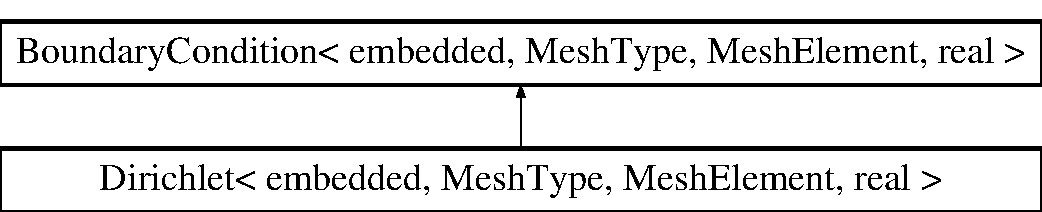
\includegraphics[height=2.000000cm]{class_boundary_condition}
\end{center}
\end{figure}
\subsection*{\-Public \-Member \-Functions}
\begin{DoxyCompactItemize}
\item 
virtual void \hyperlink{class_boundary_condition_aba7cce27bd46f51026701a11ddca04f8}{add\-To\-Triplet\-List} (\-Matrix$<$ real, \-Dynamic, \-Dynamic $>$ \&\-Kloc, \-Mesh\-Element \&element, vector$<$ \-Triplet$<$ real $>$$>$ \&triplet\-List)=0
\begin{DoxyCompactList}\small\item\em \-This is to decide if to add the \-Kloc computed to the matrix. \end{DoxyCompactList}\item 
\hypertarget{class_boundary_condition_a19b5c27271977f40146d867ff281ad24}{virtual void \hyperlink{class_boundary_condition_a19b5c27271977f40146d867ff281ad24}{assign\-Boundary\-Condition\-On\-Stiffness\-Matrix} (vector$<$ \-Triplet$<$ real $>$$>$ \&triplet\-List)=0}\label{class_boundary_condition_a19b5c27271977f40146d867ff281ad24}

\begin{DoxyCompactList}\small\item\em \-Changes the stiffness\-Matrix to keep into account the boundary condition. \end{DoxyCompactList}\item 
\hypertarget{class_boundary_condition_a6bec19c145f0cae03d30cb2c2ea80594}{virtual void \hyperlink{class_boundary_condition_a6bec19c145f0cae03d30cb2c2ea80594}{assign\-Boundary\-Condition\-On\-Known\-Term} (\-Vector\-X$<$ real $>$ \&known\-Term)=0}\label{class_boundary_condition_a6bec19c145f0cae03d30cb2c2ea80594}

\begin{DoxyCompactList}\small\item\em \-Changes the known term to keep into account the boundary condition. \end{DoxyCompactList}\end{DoxyCompactItemize}
\subsection*{\-Protected \-Member \-Functions}
\begin{DoxyCompactItemize}
\item 
\hypertarget{class_boundary_condition_a93813e79c791932c9e10eb919e0ec371}{\hyperlink{class_boundary_condition_a93813e79c791932c9e10eb919e0ec371}{\-Boundary\-Condition} (const \-Mesh\-Type \&input\-Mesh, std\-::function$<$ real(\hyperlink{class_point}{\-Point}$<$ embedded, real $>$ \&)$>$ input\-Boundary\-Function)}\label{class_boundary_condition_a93813e79c791932c9e10eb919e0ec371}

\begin{DoxyCompactList}\small\item\em \-Standard constructor. \end{DoxyCompactList}\end{DoxyCompactItemize}
\subsection*{\-Protected \-Attributes}
\begin{DoxyCompactItemize}
\item 
\hypertarget{class_boundary_condition_a14c5fa56ace975e989b5bc43f84ca048}{const \-Mesh\-Type \& {\bfseries mesh}}\label{class_boundary_condition_a14c5fa56ace975e989b5bc43f84ca048}

\item 
\hypertarget{class_boundary_condition_a0ac1cc3f463f7228e6be3171e9c0bb77}{std\-::function$<$ real(\hyperlink{class_point}{\-Point}\*
$<$ embedded, real $>$ \&)$>$ {\bfseries boundary\-Function}}\label{class_boundary_condition_a0ac1cc3f463f7228e6be3171e9c0bb77}

\end{DoxyCompactItemize}


\subsection{\-Detailed \-Description}
\subsubsection*{template$<$long embedded, typename Mesh\-Type, typename Mesh\-Element, typename real = double$>$class Boundary\-Condition$<$ embedded, Mesh\-Type, Mesh\-Element, real $>$}

\-Abstract class for \hyperlink{class_boundary_condition}{\-Boundary\-Condition}. 

\-This class does 3 main things\-:
\begin{DoxyItemize}
\item \-It processes the \-Kloc matrix after the creation from \hyperlink{class_solver}{\-Solver} (e.\-g in \hyperlink{class_dirichlet}{\-Dirichlet} condition the upper part of the stiffness matrix is diagonal and there is no need to add these terms)
\item \-Once the \-K matrix is completed it processes the full matrix to assign boundary condition (e.\-g in the same example it makes the upper part diagonal)
\item \-It imposes boundary condition also on the known term
\end{DoxyItemize}


\begin{DoxyParams}{\-Parameters}
{\em embedded} & \-Dimension of the space \\
\hline
{\em \-Mesh\-Type} & the kind of \hyperlink{class_mesh}{\-Mesh} \-I have \\
\hline
{\em \-Mesh\-Element} & \hyperlink{class_polygon}{\-Polygon} or \hyperlink{class_polyhedron}{\-Polyhedron} \\
\hline
{\em real} & double or long double \\
\hline
\end{DoxyParams}


\subsection{\-Member \-Function \-Documentation}
\hypertarget{class_boundary_condition_aba7cce27bd46f51026701a11ddca04f8}{\index{\-Boundary\-Condition@{\-Boundary\-Condition}!add\-To\-Triplet\-List@{add\-To\-Triplet\-List}}
\index{add\-To\-Triplet\-List@{add\-To\-Triplet\-List}!BoundaryCondition@{\-Boundary\-Condition}}
\subsubsection[{add\-To\-Triplet\-List}]{\setlength{\rightskip}{0pt plus 5cm}template$<$long embedded, typename Mesh\-Type , typename Mesh\-Element , typename real  = double$>$ virtual void {\bf \-Boundary\-Condition}$<$ embedded, \-Mesh\-Type, \-Mesh\-Element, real $>$\-::{\bf add\-To\-Triplet\-List} (
\begin{DoxyParamCaption}
\item[{\-Matrix$<$ real, \-Dynamic, \-Dynamic $>$ \&}]{\-Kloc, }
\item[{\-Mesh\-Element \&}]{element, }
\item[{vector$<$ \-Triplet$<$ real $>$$>$ \&}]{triplet\-List}
\end{DoxyParamCaption}
)\hspace{0.3cm}{\ttfamily  \mbox{[}pure virtual\mbox{]}}}}\label{class_boundary_condition_aba7cce27bd46f51026701a11ddca04f8}


\-This is to decide if to add the \-Kloc computed to the matrix. 

\-It depends on the boundary condition.

\-For \hyperlink{class_dirichlet}{\-Dirichlet} for example the upper part of the matrix is diagonal 

\-Implemented in \hyperlink{class_dirichlet_a8fc4c08f205989873d3c0a7fcd82cfa4}{\-Dirichlet$<$ embedded, Mesh\-Type, Mesh\-Element, real $>$}.



\-The documentation for this class was generated from the following file\-:\begin{DoxyCompactItemize}
\item 
\-Boundary\-Condition.\-h\end{DoxyCompactItemize}

\hypertarget{class_dirichlet}{}\section{Dirichlet$<$ embedded, Mesh\+Type, Mesh\+Element, real $>$ Class Template Reference}
\label{class_dirichlet}\index{Dirichlet$<$ embedded, Mesh\+Type, Mesh\+Element, real $>$@{Dirichlet$<$ embedded, Mesh\+Type, Mesh\+Element, real $>$}}


Class for \hyperlink{class_dirichlet}{Dirichlet} boundary condition.  




{\ttfamily \#include $<$Dirichlet.\+h$>$}

Inheritance diagram for Dirichlet$<$ embedded, Mesh\+Type, Mesh\+Element, real $>$\+:\begin{figure}[H]
\begin{center}
\leavevmode
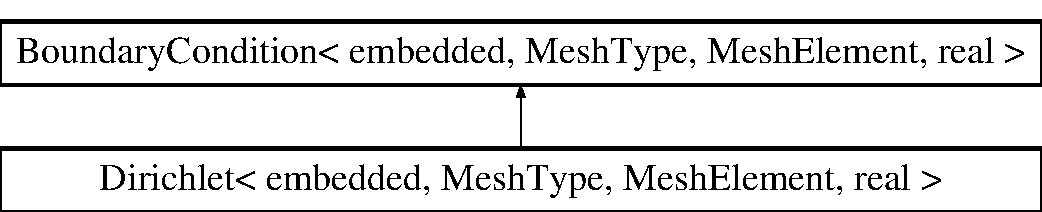
\includegraphics[height=2.000000cm]{class_dirichlet}
\end{center}
\end{figure}
\subsection*{Public Member Functions}
\begin{DoxyCompactItemize}
\item 
\hyperlink{class_dirichlet_af94781839af8702da778a451157b8b58}{Dirichlet} (const Mesh\+Type \&mesh, std\+::function$<$ real(\hyperlink{class_point}{Point}$<$ embedded, real $>$ \&)$>$ boundary\+Function)\hypertarget{class_dirichlet_af94781839af8702da778a451157b8b58}{}\label{class_dirichlet_af94781839af8702da778a451157b8b58}

\begin{DoxyCompactList}\small\item\em Standard constructor. \end{DoxyCompactList}\item 
virtual void \hyperlink{class_dirichlet_a8fc4c08f205989873d3c0a7fcd82cfa4}{add\+To\+Triplet\+List} (Matrix$<$ real, Dynamic, Dynamic $>$ \&Kloc, Mesh\+Element \&element, vector$<$ Triplet$<$ real $>$$>$ \&triplet\+List)
\begin{DoxyCompactList}\small\item\em This is to decide if to add the Kloc computed to the matrix. \end{DoxyCompactList}\item 
virtual void \hyperlink{class_dirichlet_ade7dd97b00bf71bbed49e52954f7df96}{assign\+Boundary\+Condition\+On\+Stiffness\+Matrix} (vector$<$ Triplet$<$ real $>$$>$ \&triplet\+List)\hypertarget{class_dirichlet_ade7dd97b00bf71bbed49e52954f7df96}{}\label{class_dirichlet_ade7dd97b00bf71bbed49e52954f7df96}

\begin{DoxyCompactList}\small\item\em Changes the stiffness\+Matrix to keep into account the boundary condition. \end{DoxyCompactList}\item 
virtual void \hyperlink{class_dirichlet_ac10baf3c4fa3e987a2e194899f9c4d39}{assign\+Boundary\+Condition\+On\+Known\+Term} (VectorX$<$ real $>$ \&known\+Term)\hypertarget{class_dirichlet_ac10baf3c4fa3e987a2e194899f9c4d39}{}\label{class_dirichlet_ac10baf3c4fa3e987a2e194899f9c4d39}

\begin{DoxyCompactList}\small\item\em Changes the known term to keep into account the boundary condition. \end{DoxyCompactList}\end{DoxyCompactItemize}
\subsection*{Additional Inherited Members}


\subsection{Detailed Description}
\subsubsection*{template$<$long embedded, typename Mesh\+Type, typename Mesh\+Element, typename real = double$>$\\*
class Dirichlet$<$ embedded, Mesh\+Type, Mesh\+Element, real $>$}

Class for \hyperlink{class_dirichlet}{Dirichlet} boundary condition. 


\begin{DoxyParams}{Parameters}
{\em embedded} & Dimension of the space \\
\hline
{\em Mesh\+Type} & the kind of \hyperlink{class_mesh}{Mesh} I have \\
\hline
{\em Mesh\+Element} & \hyperlink{class_polygon}{Polygon} or \hyperlink{class_polyhedron}{Polyhedron} \\
\hline
{\em real} & double or long double \\
\hline
\end{DoxyParams}


\subsection{Member Function Documentation}
\index{Dirichlet@{Dirichlet}!add\+To\+Triplet\+List@{add\+To\+Triplet\+List}}
\index{add\+To\+Triplet\+List@{add\+To\+Triplet\+List}!Dirichlet@{Dirichlet}}
\subsubsection[{\texorpdfstring{add\+To\+Triplet\+List(\+Matrix$<$ real, Dynamic, Dynamic $>$ \&\+Kloc, Mesh\+Element \&element, vector$<$ Triplet$<$ real $>$$>$ \&triplet\+List)}{addToTripletList(Matrix< real, Dynamic, Dynamic > &Kloc, MeshElement &element, vector< Triplet< real >> &tripletList)}}]{\setlength{\rightskip}{0pt plus 5cm}template$<$long embedded, typename Mesh\+Type , typename Mesh\+Element , typename real $>$ void {\bf Dirichlet}$<$ embedded, Mesh\+Type, Mesh\+Element, real $>$\+::add\+To\+Triplet\+List (
\begin{DoxyParamCaption}
\item[{Matrix$<$ real, Dynamic, Dynamic $>$ \&}]{Kloc, }
\item[{Mesh\+Element \&}]{element, }
\item[{vector$<$ Triplet$<$ real $>$$>$ \&}]{triplet\+List}
\end{DoxyParamCaption}
)\hspace{0.3cm}{\ttfamily [virtual]}}\hypertarget{class_dirichlet_a8fc4c08f205989873d3c0a7fcd82cfa4}{}\label{class_dirichlet_a8fc4c08f205989873d3c0a7fcd82cfa4}


This is to decide if to add the Kloc computed to the matrix. 

It depends on the boundary condition. 

Implements \hyperlink{class_boundary_condition_aba7cce27bd46f51026701a11ddca04f8}{Boundary\+Condition$<$ embedded, Mesh\+Type, Mesh\+Element, real $>$}.



The documentation for this class was generated from the following file\+:\begin{DoxyCompactItemize}
\item 
Dirichlet.\+h\end{DoxyCompactItemize}

\hypertarget{class_error}{\section{\-Error$<$ embedded, real $>$ \-Class \-Template \-Reference}
\label{class_error}\index{\-Error$<$ embedded, real $>$@{\-Error$<$ embedded, real $>$}}
}


\-Class to compute and display the error.  




{\ttfamily \#include $<$\-Error.\-h$>$}

\subsection*{\-Public \-Member \-Functions}
\begin{DoxyCompactItemize}
\item 
\hyperlink{class_error_aefce6e56298750a38873378411ff3d55}{\-Error} (const \-Vector\-X$<$ real $>$ \&input\-Solution, const vector$<$ shared\-\_\-ptr$<$ \hyperlink{class_mesh_point}{\-Mesh\-Point}$<$ embedded, real $>$$>$$>$ \&input\-Point\-Vector, std\-::function$<$ real(\hyperlink{class_point}{\-Point}$<$ embedded, real $>$ \&)$>$ input\-Real\-Solution\-Function, \-Sparse\-Matrix$<$ real $>$ \&input\-Stiffness\-Matrix)
\begin{DoxyCompactList}\small\item\em \-Standard constructor. \end{DoxyCompactList}\item 
real \hyperlink{class_error_a7a04e88a927c4e4c701e7f482cb97c59}{\-L\-Infinity} ()
\begin{DoxyCompactList}\small\item\em \-L infinite norm of the error. \end{DoxyCompactList}\item 
real \hyperlink{class_error_a3e3b35dcf91c1e27cee2fb546d2b9f7d}{\-H1\-Discrete} ()
\begin{DoxyCompactList}\small\item\em \-H1 discrete norm of the error. \end{DoxyCompactList}\item 
\hypertarget{class_error_a59f271538fe208ba18e7ed31d0513e83}{void \hyperlink{class_error_a59f271538fe208ba18e7ed31d0513e83}{display\-Error} ()}\label{class_error_a59f271538fe208ba18e7ed31d0513e83}

\begin{DoxyCompactList}\small\item\em \-Print the computer error. \end{DoxyCompactList}\end{DoxyCompactItemize}
\subsection*{\-Protected \-Member \-Functions}
\begin{DoxyCompactItemize}
\item 
\hypertarget{class_error_af104f894c3a83e26b85cc7a5f429dc21}{void \hyperlink{class_error_af104f894c3a83e26b85cc7a5f429dc21}{compute\-Real\-Solution} ()}\label{class_error_af104f894c3a83e26b85cc7a5f429dc21}

\begin{DoxyCompactList}\small\item\em \-This computes the exact solution, from real\-Solution\-Function. \end{DoxyCompactList}\end{DoxyCompactItemize}
\subsection*{\-Protected \-Attributes}
\begin{DoxyCompactItemize}
\item 
\hypertarget{class_error_a63e5ca94bf6ee10b531ae41fc1784ba9}{const \-Vector\-X$<$ real $>$ \& {\bfseries solution}}\label{class_error_a63e5ca94bf6ee10b531ae41fc1784ba9}

\item 
\hypertarget{class_error_a6fb9cc85ec7ed04f99bbc487d1201986}{\-Vector\-X$<$ real $>$ {\bfseries real\-Solution}}\label{class_error_a6fb9cc85ec7ed04f99bbc487d1201986}

\item 
\hypertarget{class_error_afb2549d0b0a6bfa0f81ea93a396fd462}{\-Vector\-X$<$ real $>$ {\bfseries difference}}\label{class_error_afb2549d0b0a6bfa0f81ea93a396fd462}

\item 
\hypertarget{class_error_abd75537e1d612c8f7b0ce238dc71d09a}{const vector$<$ shared\-\_\-ptr\*
$<$ \hyperlink{class_mesh_point}{\-Mesh\-Point}$<$ embedded, real $>$ $>$ $>$ \& {\bfseries point\-Vector}}\label{class_error_abd75537e1d612c8f7b0ce238dc71d09a}

\item 
\hypertarget{class_error_a9d0a0cfde3657a02ce55308a947543ee}{std\-::function$<$ real(\hyperlink{class_point}{\-Point}\*
$<$ embedded, real $>$ \&)$>$ {\bfseries real\-Solution\-Function}}\label{class_error_a9d0a0cfde3657a02ce55308a947543ee}

\item 
\hypertarget{class_error_abe45bf80209efc5704dd6311c24fbc53}{\-Sparse\-Matrix$<$ real $>$ \& {\bfseries stiffness\-Matrix}}\label{class_error_abe45bf80209efc5704dd6311c24fbc53}

\end{DoxyCompactItemize}


\subsection{\-Detailed \-Description}
\subsubsection*{template$<$long embedded, typename real = double$>$class Error$<$ embedded, real $>$}

\-Class to compute and display the error. 

\-It computes the values only in the points 2 error computed
\begin{DoxyItemize}
\item \-L infinite norm (maximum of the difference with absolute value in the points)
\item \-H1 discrete norm (u$^\wedge$\-T $\ast$ \-K $\ast$ u) 
\end{DoxyItemize}

\subsection{\-Constructor \& \-Destructor \-Documentation}
\hypertarget{class_error_aefce6e56298750a38873378411ff3d55}{\index{\-Error@{\-Error}!\-Error@{\-Error}}
\index{\-Error@{\-Error}!Error@{\-Error}}
\subsubsection[{\-Error}]{\setlength{\rightskip}{0pt plus 5cm}template$<$long embedded, typename real $>$ {\bf \-Error}$<$ embedded, real $>$\-::{\bf \-Error} (
\begin{DoxyParamCaption}
\item[{const \-Vector\-X$<$ real $>$ \&}]{input\-Solution, }
\item[{const vector$<$ shared\-\_\-ptr$<$ {\bf \-Mesh\-Point}$<$ embedded, real $>$$>$$>$ \&}]{input\-Point\-Vector, }
\item[{std\-::function$<$ real({\bf \-Point}$<$ embedded, real $>$ \&)$>$}]{input\-Real\-Solution\-Function, }
\item[{\-Sparse\-Matrix$<$ real $>$ \&}]{input\-Stiffness\-Matrix}
\end{DoxyParamCaption}
)}}\label{class_error_aefce6e56298750a38873378411ff3d55}


\-Standard constructor. 


\begin{DoxyParams}{\-Parameters}
{\em input\-Solution} & solution computed \\
\hline
{\em input\-Point\-Vector} & point\-Vector used before \\
\hline
{\em input\-Real\-Solution\-Function} & function that expresses the real solution \\
\hline
{\em input\-Stiffness\-Matrix} & used for \-H1 discrete norm \\
\hline
\end{DoxyParams}


\subsection{\-Member \-Function \-Documentation}
\hypertarget{class_error_a3e3b35dcf91c1e27cee2fb546d2b9f7d}{\index{\-Error@{\-Error}!\-H1\-Discrete@{\-H1\-Discrete}}
\index{\-H1\-Discrete@{\-H1\-Discrete}!Error@{\-Error}}
\subsubsection[{\-H1\-Discrete}]{\setlength{\rightskip}{0pt plus 5cm}template$<$long embedded, typename real $>$ real {\bf \-Error}$<$ embedded, real $>$\-::{\bf \-H1\-Discrete} (
\begin{DoxyParamCaption}
{}
\end{DoxyParamCaption}
)}}\label{class_error_a3e3b35dcf91c1e27cee2fb546d2b9f7d}


\-H1 discrete norm of the error. 

u$^\wedge$\-T $\ast$ \-K $\ast$ u where u is the solution and \-K is the stiffness matrix \hypertarget{class_error_a7a04e88a927c4e4c701e7f482cb97c59}{\index{\-Error@{\-Error}!\-L\-Infinity@{\-L\-Infinity}}
\index{\-L\-Infinity@{\-L\-Infinity}!Error@{\-Error}}
\subsubsection[{\-L\-Infinity}]{\setlength{\rightskip}{0pt plus 5cm}template$<$long embedded, typename real $>$ real {\bf \-Error}$<$ embedded, real $>$\-::{\bf \-L\-Infinity} (
\begin{DoxyParamCaption}
{}
\end{DoxyParamCaption}
)}}\label{class_error_a7a04e88a927c4e4c701e7f482cb97c59}


\-L infinite norm of the error. 

\-Maximum of the difference between points 

\-The documentation for this class was generated from the following file\-:\begin{DoxyCompactItemize}
\item 
\-Error.\-h\end{DoxyCompactItemize}

\hypertarget{class_laplace}{}\section{Laplace$<$ embedded, Mesh\+Type, Solver\+Type, Boundary\+Condition\+Type, real $>$ Class Template Reference}
\label{class_laplace}\index{Laplace$<$ embedded, Mesh\+Type, Solver\+Type, Boundary\+Condition\+Type, real $>$@{Laplace$<$ embedded, Mesh\+Type, Solver\+Type, Boundary\+Condition\+Type, real $>$}}


Class to solve a Laplacian \hyperlink{class_problem}{Problem}.  




{\ttfamily \#include $<$Laplace.\+h$>$}

Inheritance diagram for Laplace$<$ embedded, Mesh\+Type, Solver\+Type, Boundary\+Condition\+Type, real $>$\+:\begin{figure}[H]
\begin{center}
\leavevmode
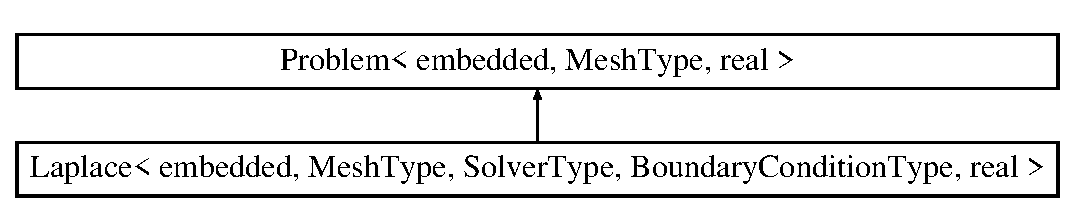
\includegraphics[height=2.000000cm]{class_laplace}
\end{center}
\end{figure}
\subsection*{Public Member Functions}
\begin{DoxyCompactItemize}
\item 
\hyperlink{class_laplace_a12701fdb17859f9348e4cd4d819a95e3}{Laplace} (const Mesh\+Type \&input\+Mesh, std\+::function$<$ real(const \hyperlink{class_point}{Point}$<$ embedded, real $>$ \&)$>$ input\+Force\+Term, std\+::function$<$ real(const \hyperlink{class_point}{Point}$<$ embedded, real $>$ \&)$>$ input\+Boundary\+Function, real input\+Diffusion\+Coeff=1)
\begin{DoxyCompactList}\small\item\em Standard constructor. \end{DoxyCompactList}\item 
void \hyperlink{class_laplace_af7da15475d7204175e8f34fbc04091d5}{compute\+Stiffness\+Matrix} ()\hypertarget{class_laplace_af7da15475d7204175e8f34fbc04091d5}{}\label{class_laplace_af7da15475d7204175e8f34fbc04091d5}

\begin{DoxyCompactList}\small\item\em Virtual method to compute the stiffness matrix. \end{DoxyCompactList}\item 
void \hyperlink{class_laplace_aa1b02086ed9e87c3aabc1b70a4ad7a82}{compute\+Known\+Term} ()\hypertarget{class_laplace_aa1b02086ed9e87c3aabc1b70a4ad7a82}{}\label{class_laplace_aa1b02086ed9e87c3aabc1b70a4ad7a82}

\begin{DoxyCompactList}\small\item\em General method. It invokes the methods of the \hyperlink{class_solver}{Solver} and \hyperlink{class_boundary_condition}{Boundary\+Condition}. \end{DoxyCompactList}\end{DoxyCompactItemize}
\subsection*{Public Attributes}
\begin{DoxyCompactItemize}
\item 
vector$<$ Triplet$<$ real $>$ $>$ \hyperlink{class_laplace_a3c7f5f7a6eaca88b6cbfee3afdfe4c07}{triplet\+List}\hypertarget{class_laplace_a3c7f5f7a6eaca88b6cbfee3afdfe4c07}{}\label{class_laplace_a3c7f5f7a6eaca88b6cbfee3afdfe4c07}

\begin{DoxyCompactList}\small\item\em Vector used to fast build the stifness\+Matrix. Triplet is a class used by Eigen library. \end{DoxyCompactList}\item 
long {\bfseries number\+Of\+Elements}\hypertarget{class_laplace_a0654b60f9552d97136a11ea7836e219b}{}\label{class_laplace_a0654b60f9552d97136a11ea7836e219b}

\item 
Boundary\+Condition\+Type {\bfseries boundary\+Condition}\hypertarget{class_laplace_a5e83c7cde7aa4051caf619d41b9642c0}{}\label{class_laplace_a5e83c7cde7aa4051caf619d41b9642c0}

\item 
Solver\+Type {\bfseries solver}\hypertarget{class_laplace_a288665cbc9433c15e61dbf08b04654a3}{}\label{class_laplace_a288665cbc9433c15e61dbf08b04654a3}

\end{DoxyCompactItemize}
\subsection*{Additional Inherited Members}


\subsection{Detailed Description}
\subsubsection*{template$<$long embedded, typename Mesh\+Type, typename Solver\+Type, typename Boundary\+Condition\+Type, typename real = double$>$\\*
class Laplace$<$ embedded, Mesh\+Type, Solver\+Type, Boundary\+Condition\+Type, real $>$}

Class to solve a Laplacian \hyperlink{class_problem}{Problem}. 


\begin{DoxyParams}{Parameters}
{\em embedded} & Dimension of the space \\
\hline
{\em Mesh\+Type} & Type of the file to read \\
\hline
{\em Solver\+Type} & Kind of \hyperlink{class_solver}{Solver} to use. Any subclass of \hyperlink{class_solver}{Solver} is allowed. \\
\hline
{\em Boundary\+Condition\+Type} & Kind of \hyperlink{class_boundary_condition}{Boundary\+Condition} to use. Any subclass of \hyperlink{class_boundary_condition}{Boundary\+Condition} is allowed. \\
\hline
{\em real} & double or long double \\
\hline
\end{DoxyParams}


\subsection{Constructor \& Destructor Documentation}
\index{Laplace@{Laplace}!Laplace@{Laplace}}
\index{Laplace@{Laplace}!Laplace@{Laplace}}
\subsubsection[{\texorpdfstring{Laplace(const Mesh\+Type \&input\+Mesh, std\+::function$<$ real(const Point$<$ embedded, real $>$ \&)$>$ input\+Force\+Term, std\+::function$<$ real(const Point$<$ embedded, real $>$ \&)$>$ input\+Boundary\+Function, real input\+Diffusion\+Coeff=1)}{Laplace(const MeshType &inputMesh, std::function< real(const Point< embedded, real > &)> inputForceTerm, std::function< real(const Point< embedded, real > &)> inputBoundaryFunction, real inputDiffusionCoeff=1)}}]{\setlength{\rightskip}{0pt plus 5cm}template$<$long embedded, typename Mesh\+Type , typename Solver\+Type , typename Boundary\+Condition\+Type , typename real  = double$>$ {\bf Laplace}$<$ embedded, Mesh\+Type, Solver\+Type, Boundary\+Condition\+Type, real $>$\+::{\bf Laplace} (
\begin{DoxyParamCaption}
\item[{const Mesh\+Type \&}]{input\+Mesh, }
\item[{std\+::function$<$ real(const {\bf Point}$<$ embedded, real $>$ \&)$>$}]{input\+Force\+Term, }
\item[{std\+::function$<$ real(const {\bf Point}$<$ embedded, real $>$ \&)$>$}]{input\+Boundary\+Function, }
\item[{real}]{input\+Diffusion\+Coeff = {\ttfamily 1}}
\end{DoxyParamCaption}
)\hspace{0.3cm}{\ttfamily [inline]}}\hypertarget{class_laplace_a12701fdb17859f9348e4cd4d819a95e3}{}\label{class_laplace_a12701fdb17859f9348e4cd4d819a95e3}


Standard constructor. 


\begin{DoxyParams}{Parameters}
{\em input\+Mesh} & \hyperlink{class_mesh}{Mesh} on which the problem is defined \\
\hline
{\em input\+Force\+Term} & Force\+Term std\+::function \\
\hline
{\em input\+Boundary\+Function} & std\+::function that expresses the boundary conditions \\
\hline
\end{DoxyParams}


The documentation for this class was generated from the following file\+:\begin{DoxyCompactItemize}
\item 
Laplace.\+h\end{DoxyCompactItemize}

\hypertarget{class_mesh}{\section{\-Mesh$<$ embedded, base\-Element, is\-Open, real $>$ \-Class \-Template \-Reference}
\label{class_mesh}\index{\-Mesh$<$ embedded, base\-Element, is\-Open, real $>$@{\-Mesh$<$ embedded, base\-Element, is\-Open, real $>$}}
}


\-Abstract class for creating a \hyperlink{class_mesh}{\-Mesh}.  




{\ttfamily \#include $<$\-Mesh.\-h$>$}

\subsection*{\-Public \-Member \-Functions}
\begin{DoxyCompactItemize}
\item 
const shared\-\_\-ptr$<$ base\-Element $>$ \& \hyperlink{class_mesh_a4a1745c0291384760349262dca8ca27c}{element} (long index) const 
\item 
const shared\-\_\-ptr$<$ \hyperlink{class_mesh_point}{\-Mesh\-Point}\*
$<$ embedded, real $>$ $>$ \& \hyperlink{class_mesh_a41e57256500b30c8a79e32ce070ff2d1}{point} (long index) const 
\item 
\hypertarget{class_mesh_ae589a7d04810b2ca182ce577c9976400}{const vector$<$ shared\-\_\-ptr\*
$<$ \hyperlink{class_mesh_point}{\-Mesh\-Point}$<$ embedded, real $>$ $>$ $>$ \& {\bfseries get\-Point\-Vector} () const }\label{class_mesh_ae589a7d04810b2ca182ce577c9976400}

\item 
\hypertarget{class_mesh_a828737450d4876e720c518ef362fa52a}{virtual real \hyperlink{class_mesh_a828737450d4876e720c518ef362fa52a}{h\-Triangle} ()}\label{class_mesh_a828737450d4876e720c518ef362fa52a}

\begin{DoxyCompactList}\small\item\em paramether h of the \hyperlink{class_mesh}{\-Mesh} \end{DoxyCompactList}\item 
void \hyperlink{class_mesh_adbdd6ff691886a2a8e9ec8192c9b0469}{initialize} (string point\-File, string connection, \-Mesh\-Type mesh\-Type=\-A\-N\-Y\-T\-H\-I\-N\-G3\-D)
\begin{DoxyCompactList}\small\item\em \-Method that calls the functions that read the file. \end{DoxyCompactList}\item 
\hypertarget{class_mesh_abb728c88ecb80918cdcc0408eb5cb0c6}{virtual void \hyperlink{class_mesh_abb728c88ecb80918cdcc0408eb5cb0c6}{set\-Point\-Vector} (string file)}\label{class_mesh_abb728c88ecb80918cdcc0408eb5cb0c6}

\begin{DoxyCompactList}\small\item\em \-It obtains the point\-Vector from file. \end{DoxyCompactList}\item 
virtual void \hyperlink{class_mesh_af6e1d08bb6a3d3a69a5ca363f8545442}{set\-Element\-Vector} (string connections, \-Mesh\-Type mesh\-Type)
\begin{DoxyCompactList}\small\item\em \-It obtains the element\-Vector from connections. \end{DoxyCompactList}\item 
virtual void \hyperlink{class_mesh_a887eb0d187f2da37b4c785d68dfcf7ad}{set\-Boundary\-Elements} ()=0
\begin{DoxyCompactList}\small\item\em \-Virtual method to keep into account the boundary elements. \end{DoxyCompactList}\item 
virtual void \hyperlink{class_mesh_a70d7cba1e66435915fb1db7c430aa44f}{set\-Remaining\-Things} ()=0
\begin{DoxyCompactList}\small\item\em \-Virtual method used to set other things, like point\-I\-Ds. \end{DoxyCompactList}\item 
\hypertarget{class_mesh_a55b0d4231dea5fce30cfe45a0a0c65f0}{virtual void {\bfseries set\-Tetrahedron\-Mesh} (string connection)}\label{class_mesh_a55b0d4231dea5fce30cfe45a0a0c65f0}

\item 
\hypertarget{class_mesh_aa06732e9d97c6753e880edda677b21b5}{virtual void \hyperlink{class_mesh_aa06732e9d97c6753e880edda677b21b5}{set\-Triangle\-Mesh} (string connection)}\label{class_mesh_aa06732e9d97c6753e880edda677b21b5}

\begin{DoxyCompactList}\small\item\em \-Read tetrahedron file type. \end{DoxyCompactList}\item 
\hypertarget{class_mesh_ae066f4f10aaaaa6d49f581dde9721c8a}{virtual void \hyperlink{class_mesh_ae066f4f10aaaaa6d49f581dde9721c8a}{set\-Anything3\-D\-Mesh} (string connection)}\label{class_mesh_ae066f4f10aaaaa6d49f581dde9721c8a}

\begin{DoxyCompactList}\small\item\em \-Read \-Triangle file type. \end{DoxyCompactList}\item 
\hypertarget{class_mesh_a2ecf67041cd4170bbe58e150c0463f22}{virtual void \hyperlink{class_mesh_a2ecf67041cd4170bbe58e150c0463f22}{set\-Anything2\-D\-Mesh} (string connection)}\label{class_mesh_a2ecf67041cd4170bbe58e150c0463f22}

\begin{DoxyCompactList}\small\item\em \-Read general polyhedron file type. \end{DoxyCompactList}\item 
\hypertarget{class_mesh_a349da9279777b5cae335524136f85567}{virtual void \hyperlink{class_mesh_a349da9279777b5cae335524136f85567}{set\-File\-Type1\-Mesh} (string connection)}\label{class_mesh_a349da9279777b5cae335524136f85567}

\begin{DoxyCompactList}\small\item\em \-Read general polygon file type. \end{DoxyCompactList}\item 
\hypertarget{class_mesh_a03cb81990255eea926696f883279935e}{virtual void \hyperlink{class_mesh_a03cb81990255eea926696f883279935e}{set\-File\-Type2\-Mesh} (string connection)}\label{class_mesh_a03cb81990255eea926696f883279935e}

\begin{DoxyCompactList}\small\item\em \-Need to be specialized. \end{DoxyCompactList}\item 
virtual void \hyperlink{class_mesh_a5cb1110ec8bf2b1d089453f873df226f}{sort} ()
\begin{DoxyCompactList}\small\item\em \-Need to be specialized. \end{DoxyCompactList}\item 
\hypertarget{class_mesh_a9c9daf07927688c3a156ee1ef0c95900}{void {\bfseries shrink\-\_\-to\-\_\-fit} ()}\label{class_mesh_a9c9daf07927688c3a156ee1ef0c95900}

\item 
\hypertarget{class_mesh_acf271beef22b8df2fb50cd9f14da7c6a}{virtual void \hyperlink{class_mesh_acf271beef22b8df2fb50cd9f14da7c6a}{write} (string output\-Points=\char`\"{}points.\-point\char`\"{}, string output\-Connections=\char`\"{}connections.\-conn\char`\"{}) const }\label{class_mesh_acf271beef22b8df2fb50cd9f14da7c6a}

\begin{DoxyCompactList}\small\item\em \-Full output to file. \end{DoxyCompactList}\item 
\hypertarget{class_mesh_a1ff4e8213296a357a0df5b7051008ae3}{virtual void \hyperlink{class_mesh_a1ff4e8213296a357a0df5b7051008ae3}{write\-Points} (string output\-File=\char`\"{}points.\-point\char`\"{}) const }\label{class_mesh_a1ff4e8213296a357a0df5b7051008ae3}

\begin{DoxyCompactList}\small\item\em \hyperlink{class_point}{\-Point} output to file. \end{DoxyCompactList}\item 
\hypertarget{class_mesh_adb3c64b4f1420c5ed0b6a74c6d9b116b}{virtual void \hyperlink{class_mesh_adb3c64b4f1420c5ed0b6a74c6d9b116b}{write\-Connections} (string output\-File=\char`\"{}connections.\-conn\char`\"{}) const }\label{class_mesh_adb3c64b4f1420c5ed0b6a74c6d9b116b}

\begin{DoxyCompactList}\small\item\em \-Connection output to file. \end{DoxyCompactList}\end{DoxyCompactItemize}
\subsection*{\-Public \-Attributes}
\begin{DoxyCompactItemize}
\item 
\hypertarget{class_mesh_af7c23d5f0561acb3fb7fae234e5f2f32}{long {\bfseries number\-Of\-Elements}}\label{class_mesh_af7c23d5f0561acb3fb7fae234e5f2f32}

\item 
\hypertarget{class_mesh_a6b2ec9290bb2a198ea28a2577a43e271}{long {\bfseries number\-Of\-Points}}\label{class_mesh_a6b2ec9290bb2a198ea28a2577a43e271}

\end{DoxyCompactItemize}
\subsection*{\-Protected \-Member \-Functions}
\begin{DoxyCompactItemize}
\item 
\hypertarget{class_mesh_ad452633f442cc10c9f9973fa82d63e58}{{\bfseries point\-Vector} (\{\})}\label{class_mesh_ad452633f442cc10c9f9973fa82d63e58}

\end{DoxyCompactItemize}
\subsection*{\-Protected \-Attributes}
\begin{DoxyCompactItemize}
\item 
\hypertarget{class_mesh_aea48e58470e3a72fcc3ee5b26f9c5315}{vector$<$ shared\-\_\-ptr$<$ base\-Element $>$ $>$ \hyperlink{class_mesh_aea48e58470e3a72fcc3ee5b26f9c5315}{element\-Vector}}\label{class_mesh_aea48e58470e3a72fcc3ee5b26f9c5315}

\begin{DoxyCompactList}\small\item\em \-Vector of \hyperlink{class_polygon}{\-Polygon} or \hyperlink{class_polyhedron}{\-Polyhedron}. \end{DoxyCompactList}\item 
\hypertarget{class_mesh_ae132c0131accc25771300cea93e26c01}{vector$<$ shared\-\_\-ptr$<$ \hyperlink{class_mesh_point}{\-Mesh\-Point}\*
$<$ embedded, real $>$ $>$ $>$ \hyperlink{class_mesh_ae132c0131accc25771300cea93e26c01}{point\-Vector}}\label{class_mesh_ae132c0131accc25771300cea93e26c01}

\begin{DoxyCompactList}\small\item\em \-Vector of the vertexes of each element. \end{DoxyCompactList}\end{DoxyCompactItemize}
\subsection*{\-Friends}
\begin{DoxyCompactItemize}
\item 
{\footnotesize template$<$long embedded2, typename base\-Element2 , \-Open\-Enum is\-Open2, typename real2 $>$ }\\ostream \& \hyperlink{class_mesh_a10337641e675a22873fcf8f0ddb7e409}{operator$<$$<$} (ostream \&os, const \hyperlink{class_mesh}{\-Mesh}$<$ embedded2, base\-Element2, is\-Open2, real2 $>$ \&mesh)
\begin{DoxyCompactList}\small\item\em \-Empty constructor. \end{DoxyCompactList}\end{DoxyCompactItemize}


\subsection{\-Detailed \-Description}
\subsubsection*{template$<$long embedded, typename base\-Element, \-Open\-Enum is\-Open = \-O\-P\-E\-N, typename real = double$>$class Mesh$<$ embedded, base\-Element, is\-Open, real $>$}

\-Abstract class for creating a \hyperlink{class_mesh}{\-Mesh}. 

\-To inherit from this\-: create a contructor, implement one of the methods to set the element\-Vector (set\-Tetrahedron\-Mesh and following) and call the method initialize in the constructor.


\begin{DoxyParams}{\-Parameters}
{\em embedded} & \-It can be 2\-D or 3\-D \\
\hline
{\em base\-Element} & typically \hyperlink{class_polygon}{\-Polygon} or \hyperlink{class_polyhedron}{\-Polyhedron} \\
\hline
{\em is\-Open} & typically open. \-It can be closed for a surface embedded in a 3\-D space \\
\hline
{\em real} & double or long double \\
\hline
\end{DoxyParams}


\subsection{\-Member \-Function \-Documentation}
\hypertarget{class_mesh_a4a1745c0291384760349262dca8ca27c}{\index{\-Mesh@{\-Mesh}!element@{element}}
\index{element@{element}!Mesh@{\-Mesh}}
\subsubsection[{element}]{\setlength{\rightskip}{0pt plus 5cm}template$<$long embedded, typename base\-Element, \-Open\-Enum is\-Open = \-O\-P\-E\-N, typename real = double$>$ const shared\-\_\-ptr$<$ base\-Element $>$ \& {\bf \-Mesh}$<$ embedded, base\-Element, is\-Open, real $>$\-::{\bf element} (
\begin{DoxyParamCaption}
\item[{long}]{index}
\end{DoxyParamCaption}
) const}}\label{class_mesh_a4a1745c0291384760349262dca8ca27c}
\begin{DoxyReturn}{\-Returns}
the element with particular index 
\end{DoxyReturn}
\hypertarget{class_mesh_adbdd6ff691886a2a8e9ec8192c9b0469}{\index{\-Mesh@{\-Mesh}!initialize@{initialize}}
\index{initialize@{initialize}!Mesh@{\-Mesh}}
\subsubsection[{initialize}]{\setlength{\rightskip}{0pt plus 5cm}template$<$long embedded, typename base\-Element , \-Open\-Enum is\-Open, typename real $>$ void {\bf \-Mesh}$<$ embedded, base\-Element, is\-Open, real $>$\-::{\bf initialize} (
\begin{DoxyParamCaption}
\item[{string}]{point\-File, }
\item[{string}]{connection, }
\item[{\-Mesh\-Type}]{mesh\-Type = {\ttfamily \-A\-N\-Y\-T\-H\-I\-N\-G3\-D}}
\end{DoxyParamCaption}
)}}\label{class_mesh_adbdd6ff691886a2a8e9ec8192c9b0469}


\-Method that calls the functions that read the file. 


\begin{DoxyParams}{\-Parameters}
{\em point\-File} & the file with the position of the \-Points \\
\hline
{\em connection} & file with th econnection between points \\
\hline
{\em mesh\-Type} & format of the file type \\
\hline
\end{DoxyParams}
\hypertarget{class_mesh_a41e57256500b30c8a79e32ce070ff2d1}{\index{\-Mesh@{\-Mesh}!point@{point}}
\index{point@{point}!Mesh@{\-Mesh}}
\subsubsection[{point}]{\setlength{\rightskip}{0pt plus 5cm}template$<$long embedded, typename base\-Element , \-Open\-Enum is\-Open, typename real $>$ const shared\-\_\-ptr$<$ {\bf \-Mesh\-Point}$<$ embedded, real $>$ $>$ \& {\bf \-Mesh}$<$ embedded, base\-Element, is\-Open, real $>$\-::{\bf point} (
\begin{DoxyParamCaption}
\item[{long}]{index}
\end{DoxyParamCaption}
) const}}\label{class_mesh_a41e57256500b30c8a79e32ce070ff2d1}
\begin{DoxyReturn}{\-Returns}
the \hyperlink{class_mesh_point}{\-Mesh\-Point} with a particular index 
\end{DoxyReturn}
\hypertarget{class_mesh_a887eb0d187f2da37b4c785d68dfcf7ad}{\index{\-Mesh@{\-Mesh}!set\-Boundary\-Elements@{set\-Boundary\-Elements}}
\index{set\-Boundary\-Elements@{set\-Boundary\-Elements}!Mesh@{\-Mesh}}
\subsubsection[{set\-Boundary\-Elements}]{\setlength{\rightskip}{0pt plus 5cm}template$<$long embedded, typename base\-Element, \-Open\-Enum is\-Open = \-O\-P\-E\-N, typename real = double$>$ virtual void {\bf \-Mesh}$<$ embedded, base\-Element, is\-Open, real $>$\-::{\bf set\-Boundary\-Elements} (
\begin{DoxyParamCaption}
{}
\end{DoxyParamCaption}
)\hspace{0.3cm}{\ttfamily  \mbox{[}pure virtual\mbox{]}}}}\label{class_mesh_a887eb0d187f2da37b4c785d68dfcf7ad}


\-Virtual method to keep into account the boundary elements. 



\-Implemented in \hyperlink{class_mesh2_d_ac6408b5999b1deddbbd137dc8bd9e1cd}{\-Mesh2\-D$<$ real $>$}, and \hyperlink{class_mesh3_d_a5c90136ef98ac86c4bbd51eaa6c9b811}{\-Mesh3\-D$<$ real $>$}.

\hypertarget{class_mesh_af6e1d08bb6a3d3a69a5ca363f8545442}{\index{\-Mesh@{\-Mesh}!set\-Element\-Vector@{set\-Element\-Vector}}
\index{set\-Element\-Vector@{set\-Element\-Vector}!Mesh@{\-Mesh}}
\subsubsection[{set\-Element\-Vector}]{\setlength{\rightskip}{0pt plus 5cm}template$<$long embedded, typename base\-Element , \-Open\-Enum is\-Open, typename real $>$ void {\bf \-Mesh}$<$ embedded, base\-Element, is\-Open, real $>$\-::{\bf set\-Element\-Vector} (
\begin{DoxyParamCaption}
\item[{string}]{connections, }
\item[{\-Mesh\-Type}]{mesh\-Type}
\end{DoxyParamCaption}
)\hspace{0.3cm}{\ttfamily  \mbox{[}virtual\mbox{]}}}}\label{class_mesh_af6e1d08bb6a3d3a69a5ca363f8545442}


\-It obtains the element\-Vector from connections. 

\-Then it calls the appropriate method to read the connection file \hypertarget{class_mesh_a70d7cba1e66435915fb1db7c430aa44f}{\index{\-Mesh@{\-Mesh}!set\-Remaining\-Things@{set\-Remaining\-Things}}
\index{set\-Remaining\-Things@{set\-Remaining\-Things}!Mesh@{\-Mesh}}
\subsubsection[{set\-Remaining\-Things}]{\setlength{\rightskip}{0pt plus 5cm}template$<$long embedded, typename base\-Element, \-Open\-Enum is\-Open = \-O\-P\-E\-N, typename real = double$>$ virtual void {\bf \-Mesh}$<$ embedded, base\-Element, is\-Open, real $>$\-::{\bf set\-Remaining\-Things} (
\begin{DoxyParamCaption}
{}
\end{DoxyParamCaption}
)\hspace{0.3cm}{\ttfamily  \mbox{[}pure virtual\mbox{]}}}}\label{class_mesh_a70d7cba1e66435915fb1db7c430aa44f}


\-Virtual method used to set other things, like point\-I\-Ds. 



\-Implemented in \hyperlink{class_mesh2_d_ae52c22a91d85fdb99955bf57162f6dac}{\-Mesh2\-D$<$ real $>$}, and \hyperlink{class_mesh3_d_ab13f81c133cff51c5e386db23c5ec685}{\-Mesh3\-D$<$ real $>$}.

\hypertarget{class_mesh_a5cb1110ec8bf2b1d089453f873df226f}{\index{\-Mesh@{\-Mesh}!sort@{sort}}
\index{sort@{sort}!Mesh@{\-Mesh}}
\subsubsection[{sort}]{\setlength{\rightskip}{0pt plus 5cm}template$<$long embedded, typename base\-Element , \-Open\-Enum is\-Open, typename real $>$ void {\bf \-Mesh}$<$ embedded, base\-Element, is\-Open, real $>$\-::{\bf sort} (
\begin{DoxyParamCaption}
{}
\end{DoxyParamCaption}
)\hspace{0.3cm}{\ttfamily  \mbox{[}virtual\mbox{]}}}}\label{class_mesh_a5cb1110ec8bf2b1d089453f873df226f}


\-Need to be specialized. 

\-Sort the point\-Vector based on point\-I\-D 

\subsection{\-Friends \-And \-Related \-Function \-Documentation}
\hypertarget{class_mesh_a10337641e675a22873fcf8f0ddb7e409}{\index{\-Mesh@{\-Mesh}!operator$<$$<$@{operator$<$$<$}}
\index{operator$<$$<$@{operator$<$$<$}!Mesh@{\-Mesh}}
\subsubsection[{operator$<$$<$}]{\setlength{\rightskip}{0pt plus 5cm}template$<$long embedded, typename base\-Element, \-Open\-Enum is\-Open = \-O\-P\-E\-N, typename real = double$>$ template$<$long embedded2, typename base\-Element2 , \-Open\-Enum is\-Open2, typename real2 $>$ ostream\& operator$<$$<$ (
\begin{DoxyParamCaption}
\item[{ostream \&}]{os, }
\item[{const {\bf \-Mesh}$<$ embedded2, base\-Element2, is\-Open2, real2 $>$ \&}]{mesh}
\end{DoxyParamCaption}
)\hspace{0.3cm}{\ttfamily  \mbox{[}friend\mbox{]}}}}\label{class_mesh_a10337641e675a22873fcf8f0ddb7e409}


\-Empty constructor. 

\-Output operator 

\-The documentation for this class was generated from the following file\-:\begin{DoxyCompactItemize}
\item 
\-Mesh.\-h\end{DoxyCompactItemize}

\hypertarget{class_mesh2_d}{}\section{Mesh2D$<$ real $>$ Class Template Reference}
\label{class_mesh2_d}\index{Mesh2\+D$<$ real $>$@{Mesh2\+D$<$ real $>$}}


Specialized class for 2D \hyperlink{class_mesh}{Mesh}.  




{\ttfamily \#include $<$Mesh2\+D.\+h$>$}

Inheritance diagram for Mesh2D$<$ real $>$\+:\begin{figure}[H]
\begin{center}
\leavevmode
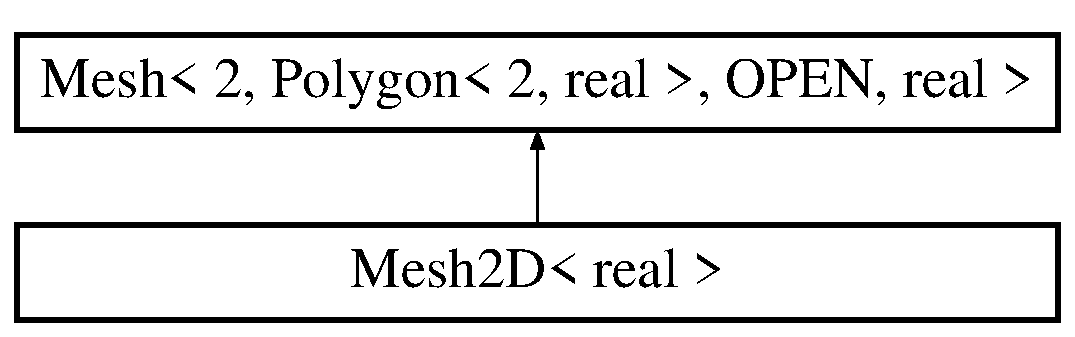
\includegraphics[height=2.000000cm]{class_mesh2_d}
\end{center}
\end{figure}
\subsection*{Public Member Functions}
\begin{DoxyCompactItemize}
\item 
\hyperlink{class_mesh2_d_a98d286dea8fdf7b908b3a56991beca47}{Mesh2D} (string point\+File, string connection\+File, Mesh\+Type mesh\+Type=A\+N\+Y\+T\+H\+I\+N\+G2D)\hypertarget{class_mesh2_d_a98d286dea8fdf7b908b3a56991beca47}{}\label{class_mesh2_d_a98d286dea8fdf7b908b3a56991beca47}

\begin{DoxyCompactList}\small\item\em Constructor with input file. \end{DoxyCompactList}\item 
{\footnotesize template$<$typename... Args$>$ }\\shared\+\_\+ptr$<$ \hyperlink{class_polygon}{Polygon}$<$ 2, real $>$ $>$ \hyperlink{class_mesh2_d_a08651a8b7f996ea4d8896bd0802d6f24}{new\+Polygon} (Args...\+arguments)\hypertarget{class_mesh2_d_a08651a8b7f996ea4d8896bd0802d6f24}{}\label{class_mesh2_d_a08651a8b7f996ea4d8896bd0802d6f24}

\begin{DoxyCompactList}\small\item\em Method to add a \hyperlink{class_polygon}{Polygon} to the \hyperlink{class_mesh}{Mesh} after having read it. \end{DoxyCompactList}\item 
virtual void \hyperlink{class_mesh2_d_a6cf7a73abadd08ecd18d6f35c7b644c3}{set\+Anything2\+D\+Mesh} (string connection)\hypertarget{class_mesh2_d_a6cf7a73abadd08ecd18d6f35c7b644c3}{}\label{class_mesh2_d_a6cf7a73abadd08ecd18d6f35c7b644c3}

\begin{DoxyCompactList}\small\item\em Specilization of the method to read A\+N\+Y\+T\+H\+I\+N\+G2D file. \end{DoxyCompactList}\item 
virtual void \hyperlink{class_mesh2_d_ac6408b5999b1deddbbd137dc8bd9e1cd}{set\+Boundary\+Elements} ()
\begin{DoxyCompactList}\small\item\em Specilization of the method. \end{DoxyCompactList}\item 
virtual void \hyperlink{class_mesh2_d_ae52c22a91d85fdb99955bf57162f6dac}{set\+Remaining\+Things} ()
\begin{DoxyCompactList}\small\item\em Specilization of the method. \end{DoxyCompactList}\item 
void {\bfseries shrink\+\_\+to\+\_\+fit} ()\hypertarget{class_mesh2_d_a06fba3c3fc41d127a8238d4a1b7972a3}{}\label{class_mesh2_d_a06fba3c3fc41d127a8238d4a1b7972a3}

\end{DoxyCompactItemize}
\subsection*{Public Attributes}
\begin{DoxyCompactItemize}
\item 
long {\bfseries number\+Of\+Boundary\+Points}\hypertarget{class_mesh2_d_a3c1c3c7ab2139d81e6166bc493365191}{}\label{class_mesh2_d_a3c1c3c7ab2139d81e6166bc493365191}

\end{DoxyCompactItemize}
\subsection*{Additional Inherited Members}


\subsection{Detailed Description}
\subsubsection*{template$<$typename real = double$>$\\*
class Mesh2\+D$<$ real $>$}

Specialized class for 2D \hyperlink{class_mesh}{Mesh}. 

Base\+Element is a \hyperlink{class_polygon}{Polygon} 

\subsection{Member Function Documentation}
\index{Mesh2D@{Mesh2D}!set\+Boundary\+Elements@{set\+Boundary\+Elements}}
\index{set\+Boundary\+Elements@{set\+Boundary\+Elements}!Mesh2D@{Mesh2D}}
\subsubsection[{\texorpdfstring{set\+Boundary\+Elements()}{setBoundaryElements()}}]{\setlength{\rightskip}{0pt plus 5cm}template$<$typename real $>$ void {\bf Mesh2D}$<$ real $>$\+::set\+Boundary\+Elements (
\begin{DoxyParamCaption}
{}
\end{DoxyParamCaption}
)\hspace{0.3cm}{\ttfamily [virtual]}}\hypertarget{class_mesh2_d_ac6408b5999b1deddbbd137dc8bd9e1cd}{}\label{class_mesh2_d_ac6408b5999b1deddbbd137dc8bd9e1cd}


Specilization of the method. 

It uses the pair\+Vector to accelerate the computation 

Implements \hyperlink{class_mesh_a887eb0d187f2da37b4c785d68dfcf7ad}{Mesh$<$ 2, Polygon$<$ 2, real $>$, O\+P\+E\+N, real $>$}.

\index{Mesh2D@{Mesh2D}!set\+Remaining\+Things@{set\+Remaining\+Things}}
\index{set\+Remaining\+Things@{set\+Remaining\+Things}!Mesh2D@{Mesh2D}}
\subsubsection[{\texorpdfstring{set\+Remaining\+Things()}{setRemainingThings()}}]{\setlength{\rightskip}{0pt plus 5cm}template$<$typename real $>$ void {\bf Mesh2D}$<$ real $>$\+::set\+Remaining\+Things (
\begin{DoxyParamCaption}
{}
\end{DoxyParamCaption}
)\hspace{0.3cm}{\ttfamily [virtual]}}\hypertarget{class_mesh2_d_ae52c22a91d85fdb99955bf57162f6dac}{}\label{class_mesh2_d_ae52c22a91d85fdb99955bf57162f6dac}


Specilization of the method. 

It sets point\+I\+Ds and number\+Of\+Boundary\+Points 

Implements \hyperlink{class_mesh_a70d7cba1e66435915fb1db7c430aa44f}{Mesh$<$ 2, Polygon$<$ 2, real $>$, O\+P\+E\+N, real $>$}.



The documentation for this class was generated from the following file\+:\begin{DoxyCompactItemize}
\item 
Mesh2\+D.\+h\end{DoxyCompactItemize}

\hypertarget{class_mesh3_d}{\section{\-Mesh3\-D$<$ real $>$ \-Class \-Template \-Reference}
\label{class_mesh3_d}\index{\-Mesh3\-D$<$ real $>$@{\-Mesh3\-D$<$ real $>$}}
}


\-Specialized class for 3\-D \hyperlink{class_mesh}{\-Mesh}.  




{\ttfamily \#include $<$\-Mesh3\-D.\-h$>$}

\-Inheritance diagram for \-Mesh3\-D$<$ real $>$\-:\begin{figure}[H]
\begin{center}
\leavevmode
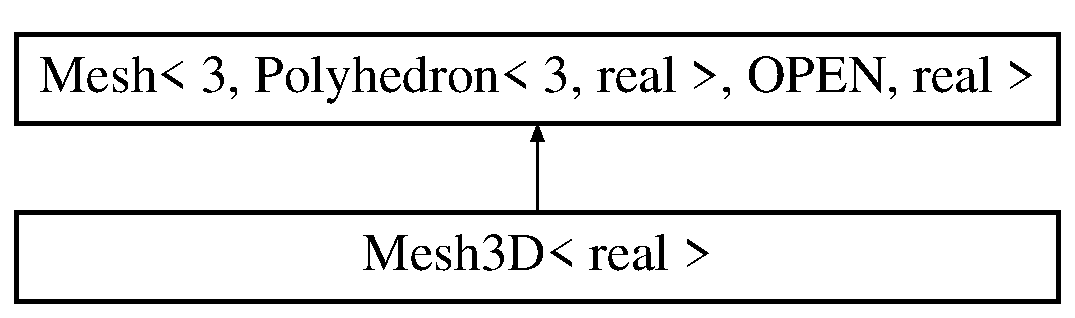
\includegraphics[height=2.000000cm]{class_mesh3_d}
\end{center}
\end{figure}
\subsection*{\-Public \-Member \-Functions}
\begin{DoxyCompactItemize}
\item 
\hypertarget{class_mesh3_d_ab5b158493bd041915b32ff7c17570a8e}{\hyperlink{class_mesh3_d_ab5b158493bd041915b32ff7c17570a8e}{\-Mesh3\-D} (string point\-File, string connection\-File, \-Mesh\-Type mesh\-Type=\-A\-N\-Y\-T\-H\-I\-N\-G3\-D)}\label{class_mesh3_d_ab5b158493bd041915b32ff7c17570a8e}

\begin{DoxyCompactList}\small\item\em \-Constructor with input file. \end{DoxyCompactList}\item 
\hypertarget{class_mesh3_d_abbc268d8c9008d4d2b83bc684530764e}{{\bfseries number\-Of\-Polygons} (0)}\label{class_mesh3_d_abbc268d8c9008d4d2b83bc684530764e}

\item 
\hypertarget{class_mesh3_d_ae7bd0fd5fc65d2217a2cdb2180fa55f7}{{\bfseries number\-Of\-Boundary\-Points} (0)}\label{class_mesh3_d_ae7bd0fd5fc65d2217a2cdb2180fa55f7}

\item 
{\footnotesize template$<$typename... \-Args$>$ }\\shared\-\_\-ptr$<$ \hyperlink{class_polygon}{\-Polygon}$<$ 3, real $>$ $>$ \hyperlink{class_mesh3_d_a34d811780e44e448dc45f7142078a1d0}{new\-Face} (\-Args...\-arguments)
\begin{DoxyCompactList}\small\item\em \-Method to create a \hyperlink{class_polygon}{\-Polygon} after having read it. \end{DoxyCompactList}\item 
virtual void \hyperlink{class_mesh3_d_a5c90136ef98ac86c4bbd51eaa6c9b811}{set\-Boundary\-Elements} ()
\begin{DoxyCompactList}\small\item\em \-Specilization of the method. \end{DoxyCompactList}\item 
\hypertarget{class_mesh3_d_ab13f81c133cff51c5e386db23c5ec685}{virtual void \hyperlink{class_mesh3_d_ab13f81c133cff51c5e386db23c5ec685}{set\-Remaining\-Things} ()}\label{class_mesh3_d_ab13f81c133cff51c5e386db23c5ec685}

\begin{DoxyCompactList}\small\item\em \-Specilization of the method. \end{DoxyCompactList}\item 
virtual void \hyperlink{class_mesh3_d_ad2ce515add93ae41902537fba24a09a2}{set\-Tetrahedron\-Mesh} (string connection)
\begin{DoxyCompactList}\small\item\em \hyperlink{class_mesh}{\-Mesh} of \-T\-E\-T\-R\-A\-H\-E\-D\-R\-O\-N type. \end{DoxyCompactList}\item 
virtual void \hyperlink{class_mesh3_d_a449dba8699a5e4e1ab101a79e411f443}{set\-Anything3\-D\-Mesh} (string connection)
\begin{DoxyCompactList}\small\item\em \hyperlink{class_mesh}{\-Mesh} of \-A\-N\-Y\-T\-H\-I\-N\-G3\-D type. \end{DoxyCompactList}\item 
\hypertarget{class_mesh3_d_a9cdf6867d5a6c53ab50d793360b00132}{void {\bfseries shrink\-\_\-to\-\_\-fit} ()}\label{class_mesh3_d_a9cdf6867d5a6c53ab50d793360b00132}

\item 
\hypertarget{class_mesh3_d_ac43faf1c99509f0aba384eda248202f9}{const shared\-\_\-ptr$<$ \hyperlink{class_polygon}{\-Polygon}\*
$<$ 3, real $>$ $>$ \& \hyperlink{class_mesh3_d_ac43faf1c99509f0aba384eda248202f9}{polygon} (long index) const }\label{class_mesh3_d_ac43faf1c99509f0aba384eda248202f9}

\begin{DoxyCompactList}\small\item\em \-Get \hyperlink{class_polygon}{\-Polygon} with index. \end{DoxyCompactList}\end{DoxyCompactItemize}
\subsection*{\-Public \-Attributes}
\begin{DoxyCompactItemize}
\item 
\hypertarget{class_mesh3_d_a4d5bd1d28908b333881fa0d9f8f50a9b}{long {\bfseries number\-Of\-Polygons}}\label{class_mesh3_d_a4d5bd1d28908b333881fa0d9f8f50a9b}

\item 
\hypertarget{class_mesh3_d_a9a047727135fd08147e4eeadc1f20f96}{long {\bfseries number\-Of\-Boundary\-Points}}\label{class_mesh3_d_a9a047727135fd08147e4eeadc1f20f96}

\end{DoxyCompactItemize}
\subsection*{\-Protected \-Attributes}
\begin{DoxyCompactItemize}
\item 
\hypertarget{class_mesh3_d_a175584ad52fb0bd5162cc27b0d3359b9}{vector$<$ shared\-\_\-ptr$<$ \hyperlink{class_polygon}{\-Polygon}\*
$<$ 3, real $>$ $>$ $>$ \hyperlink{class_mesh3_d_a175584ad52fb0bd5162cc27b0d3359b9}{polygon\-Vector}}\label{class_mesh3_d_a175584ad52fb0bd5162cc27b0d3359b9}

\begin{DoxyCompactList}\small\item\em \-Vector of all the \hyperlink{class_polyhedron}{\-Polyhedron} faces. \end{DoxyCompactList}\end{DoxyCompactItemize}


\subsection{\-Detailed \-Description}
\subsubsection*{template$<$typename real = double$>$class Mesh3\-D$<$ real $>$}

\-Specialized class for 3\-D \hyperlink{class_mesh}{\-Mesh}. 

\-Base\-Element is a \hyperlink{class_polyhedron}{\-Polyhedron}.

2 possibilities of file type\-: tetrahedron and anything3\-D. \-In the first for each \hyperlink{class_polyhedron}{\-Polyhedron} only the vertex are specified in the connection file. \-In the second for each \hyperlink{class_polyhedron}{\-Polyhedron} all the faces are specified. 

\subsection{\-Member \-Function \-Documentation}
\hypertarget{class_mesh3_d_a34d811780e44e448dc45f7142078a1d0}{\index{\-Mesh3\-D@{\-Mesh3\-D}!new\-Face@{new\-Face}}
\index{new\-Face@{new\-Face}!Mesh3D@{\-Mesh3\-D}}
\subsubsection[{new\-Face}]{\setlength{\rightskip}{0pt plus 5cm}template$<$typename real $>$ template$<$typename... \-Args$>$ shared\-\_\-ptr$<$ {\bf \-Polygon}$<$ 3, real $>$ $>$ {\bf \-Mesh3\-D}$<$ real $>$\-::{\bf new\-Face} (
\begin{DoxyParamCaption}
\item[{\-Args...}]{arguments}
\end{DoxyParamCaption}
)}}\label{class_mesh3_d_a34d811780e44e448dc45f7142078a1d0}


\-Method to create a \hyperlink{class_polygon}{\-Polygon} after having read it. 

\-It calls make\-\_\-shared\-\_\-\-Polygon. \-It also checks if the \hyperlink{class_polygon}{\-Polygon} is on the boundary or not. \-It's faster to do it now, rather than after having read everything. \hypertarget{class_mesh3_d_a449dba8699a5e4e1ab101a79e411f443}{\index{\-Mesh3\-D@{\-Mesh3\-D}!set\-Anything3\-D\-Mesh@{set\-Anything3\-D\-Mesh}}
\index{set\-Anything3\-D\-Mesh@{set\-Anything3\-D\-Mesh}!Mesh3D@{\-Mesh3\-D}}
\subsubsection[{set\-Anything3\-D\-Mesh}]{\setlength{\rightskip}{0pt plus 5cm}template$<$typename real $>$ void {\bf \-Mesh3\-D}$<$ real $>$\-::{\bf set\-Anything3\-D\-Mesh} (
\begin{DoxyParamCaption}
\item[{string}]{connection}
\end{DoxyParamCaption}
)\hspace{0.3cm}{\ttfamily  \mbox{[}virtual\mbox{]}}}}\label{class_mesh3_d_a449dba8699a5e4e1ab101a79e411f443}


\hyperlink{class_mesh}{\-Mesh} of \-A\-N\-Y\-T\-H\-I\-N\-G3\-D type. 

e.\-g. \-This is a \hyperlink{class_polyhedron}{\-Polyhedron}, where 120 is the 120th point in the point\-Vector\-: 120,124,119,155 

\-Reimplemented from \hyperlink{class_mesh_ae066f4f10aaaaa6d49f581dde9721c8a}{\-Mesh$<$ 3, Polyhedron$<$ 3, real $>$, O\-P\-E\-N, real $>$}.

\hypertarget{class_mesh3_d_a5c90136ef98ac86c4bbd51eaa6c9b811}{\index{\-Mesh3\-D@{\-Mesh3\-D}!set\-Boundary\-Elements@{set\-Boundary\-Elements}}
\index{set\-Boundary\-Elements@{set\-Boundary\-Elements}!Mesh3D@{\-Mesh3\-D}}
\subsubsection[{set\-Boundary\-Elements}]{\setlength{\rightskip}{0pt plus 5cm}template$<$typename real $>$ void {\bf \-Mesh3\-D}$<$ real $>$\-::{\bf set\-Boundary\-Elements} (
\begin{DoxyParamCaption}
{}
\end{DoxyParamCaption}
)\hspace{0.3cm}{\ttfamily  \mbox{[}virtual\mbox{]}}}}\label{class_mesh3_d_a5c90136ef98ac86c4bbd51eaa6c9b811}


\-Specilization of the method. 

\-Simple method, the main work is done in new\-Face 

\-Implements \hyperlink{class_mesh_a887eb0d187f2da37b4c785d68dfcf7ad}{\-Mesh$<$ 3, Polyhedron$<$ 3, real $>$, O\-P\-E\-N, real $>$}.

\hypertarget{class_mesh3_d_ad2ce515add93ae41902537fba24a09a2}{\index{\-Mesh3\-D@{\-Mesh3\-D}!set\-Tetrahedron\-Mesh@{set\-Tetrahedron\-Mesh}}
\index{set\-Tetrahedron\-Mesh@{set\-Tetrahedron\-Mesh}!Mesh3D@{\-Mesh3\-D}}
\subsubsection[{set\-Tetrahedron\-Mesh}]{\setlength{\rightskip}{0pt plus 5cm}template$<$typename real $>$ void {\bf \-Mesh3\-D}$<$ real $>$\-::{\bf set\-Tetrahedron\-Mesh} (
\begin{DoxyParamCaption}
\item[{string}]{connection}
\end{DoxyParamCaption}
)\hspace{0.3cm}{\ttfamily  \mbox{[}virtual\mbox{]}}}}\label{class_mesh3_d_ad2ce515add93ae41902537fba24a09a2}


\hyperlink{class_mesh}{\-Mesh} of \-T\-E\-T\-R\-A\-H\-E\-D\-R\-O\-N type. 

e.\-g. \-This is a \hyperlink{class_polyhedron}{\-Polyhedron}, where 10 is the 10th point in the point\-Vector and each ';' describe a face\-: 1,10,13,4;1,10,11,2;10,13,14,11;13,4,5,14;4,1,2,5;2,11,14,5 

\-Reimplemented from \hyperlink{class_mesh}{\-Mesh$<$ 3, Polyhedron$<$ 3, real $>$, O\-P\-E\-N, real $>$}.



\-The documentation for this class was generated from the following file\-:\begin{DoxyCompactItemize}
\item 
\-Mesh3\-D.\-h\end{DoxyCompactItemize}

\hypertarget{class_mesh_point}{}\section{Mesh\+Point$<$ embedded, real $>$ Class Template Reference}
\label{class_mesh_point}\index{Mesh\+Point$<$ embedded, real $>$@{Mesh\+Point$<$ embedded, real $>$}}


Class to represent a \hyperlink{class_point}{Point} belonging to a \hyperlink{class_mesh}{Mesh}.  




{\ttfamily \#include $<$Mesh\+Point.\+h$>$}

Inheritance diagram for Mesh\+Point$<$ embedded, real $>$\+:\begin{figure}[H]
\begin{center}
\leavevmode
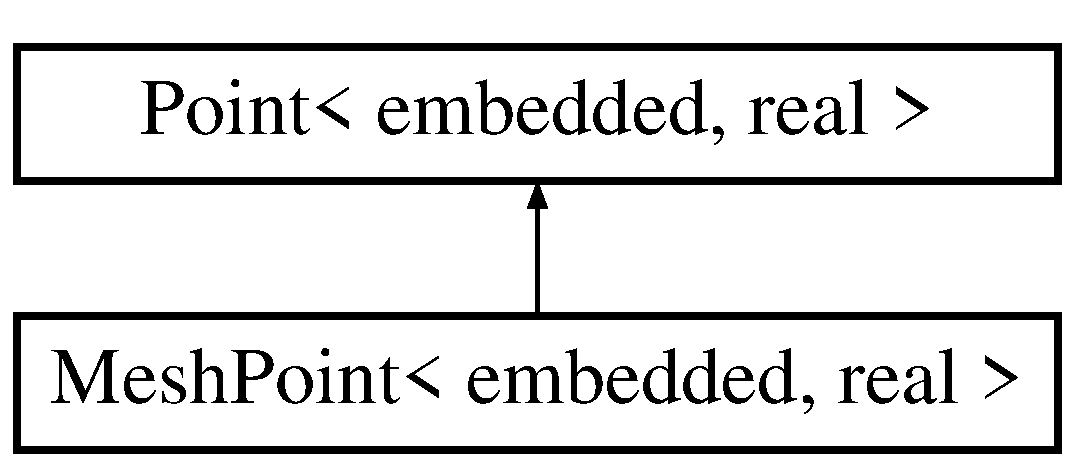
\includegraphics[height=2.000000cm]{class_mesh_point}
\end{center}
\end{figure}
\subsection*{Public Member Functions}
\begin{DoxyCompactItemize}
\item 
\hyperlink{class_mesh_point_aa172f99891420d566250fa3df4f69263}{Mesh\+Point} (const array$<$ real, embedded $>$ \&input\+Array)\hypertarget{class_mesh_point_aa172f99891420d566250fa3df4f69263}{}\label{class_mesh_point_aa172f99891420d566250fa3df4f69263}

\begin{DoxyCompactList}\small\item\em Constructor from array of coordinates. \end{DoxyCompactList}\item 
{\footnotesize template$<$typename... Args$>$ }\\\hyperlink{class_mesh_point_a9fce0473490e3f1447d6adc100df166a}{Mesh\+Point} (Args...\+arguments)
\begin{DoxyCompactList}\small\item\em Empty constructor. \end{DoxyCompactList}\item 
void \hyperlink{class_mesh_point_ad13eb69436888b26b2d8a4eda9ebf21b}{add\+Polygon} (weak\+\_\+ptr$<$ \hyperlink{class_polygon}{Polygon}$<$ embedded, real $>$$>$ input\+Polygon)\hypertarget{class_mesh_point_ad13eb69436888b26b2d8a4eda9ebf21b}{}\label{class_mesh_point_ad13eb69436888b26b2d8a4eda9ebf21b}

\begin{DoxyCompactList}\small\item\em It insert in polygon vector a new \hyperlink{class_polygon}{Polygon}. \end{DoxyCompactList}\item 
void \hyperlink{class_mesh_point_a60b10a88168d410b63a191fa297ba088}{add\+Polyhedron} (weak\+\_\+ptr$<$ \hyperlink{class_polyhedron}{Polyhedron}$<$ embedded, real $>$$>$ input\+Polyhedron)\hypertarget{class_mesh_point_a60b10a88168d410b63a191fa297ba088}{}\label{class_mesh_point_a60b10a88168d410b63a191fa297ba088}

\begin{DoxyCompactList}\small\item\em It insert in polyhedron vector a new \hyperlink{class_polyhedron}{Polyhedron}. \end{DoxyCompactList}\item 
void {\bfseries shrink\+\_\+to\+\_\+fit} ()\hypertarget{class_mesh_point_a3d9ebecff4fe87012077db61e25afba1}{}\label{class_mesh_point_a3d9ebecff4fe87012077db61e25afba1}

\item 
long {\bfseries get\+Point\+ID} () const \hypertarget{class_mesh_point_ab373939208adf6f3a6720337b72ab4df}{}\label{class_mesh_point_ab373939208adf6f3a6720337b72ab4df}

\item 
void {\bfseries set\+Point\+ID} (long input\+Point\+ID)\hypertarget{class_mesh_point_a9fb3ec58099e4e711643cc0fae370f79}{}\label{class_mesh_point_a9fb3ec58099e4e711643cc0fae370f79}

\item 
bool {\bfseries get\+Is\+Boundary} () const \hypertarget{class_mesh_point_a53fc7a6ea17475aafeec206c9de3edd8}{}\label{class_mesh_point_a53fc7a6ea17475aafeec206c9de3edd8}

\item 
void {\bfseries set\+Is\+Boundary} (bool input\+Is\+Boundary)\hypertarget{class_mesh_point_a2c0fb6d2c9eea8ff733c694eead116bc}{}\label{class_mesh_point_a2c0fb6d2c9eea8ff733c694eead116bc}

\item 
long {\bfseries number\+Of\+Polygons} () const \hypertarget{class_mesh_point_a05dd421cf0eb43450b5b36e6460004b6}{}\label{class_mesh_point_a05dd421cf0eb43450b5b36e6460004b6}

\item 
long \hyperlink{class_mesh_point_a42eaf370ee97316363f183b2ed2fea30}{number\+Of\+Polyhedrons} () const \hypertarget{class_mesh_point_a42eaf370ee97316363f183b2ed2fea30}{}\label{class_mesh_point_a42eaf370ee97316363f183b2ed2fea30}

\begin{DoxyCompactList}\small\item\em Number of Polygons with this as vertex. \end{DoxyCompactList}\item 
const weak\+\_\+ptr$<$ \hyperlink{class_polygon}{Polygon}$<$ embedded, real $>$ $>$ \& \hyperlink{class_mesh_point_afccab1b0b35b3823a69f2cc90cc6a043}{polygon} (long index) const \hypertarget{class_mesh_point_afccab1b0b35b3823a69f2cc90cc6a043}{}\label{class_mesh_point_afccab1b0b35b3823a69f2cc90cc6a043}

\begin{DoxyCompactList}\small\item\em Number of Polyhedorns with this as vertex. \end{DoxyCompactList}\item 
const weak\+\_\+ptr$<$ \hyperlink{class_polyhedron}{Polyhedron}$<$ embedded, real $>$ $>$ \& \hyperlink{class_mesh_point_a7bca0a9727c94dad3d9fef2aac8e310b}{polyhedron} (long index) const \hypertarget{class_mesh_point_a7bca0a9727c94dad3d9fef2aac8e310b}{}\label{class_mesh_point_a7bca0a9727c94dad3d9fef2aac8e310b}

\begin{DoxyCompactList}\small\item\em Get a weak pointer to a \hyperlink{class_polygon}{Polygon} in polygon\+Vector. \end{DoxyCompactList}\item 
bool \hyperlink{class_mesh_point_a429995d48aa19e82d8beccf3068a8851}{operator$<$} (\hyperlink{class_mesh_point}{Mesh\+Point}$<$ embedded, real $>$ \&input\+Point)
\begin{DoxyCompactList}\small\item\em Get a weak pointer to a \hyperlink{class_polyhedron}{Polyhedron} in polyhedron\+Vector. \end{DoxyCompactList}\end{DoxyCompactItemize}
\subsection*{Protected Attributes}
\begin{DoxyCompactItemize}
\item 
long \hyperlink{class_mesh_point_a474d09b4818c37c554f2d89a86da4d10}{point\+ID}\hypertarget{class_mesh_point_a474d09b4818c37c554f2d89a86da4d10}{}\label{class_mesh_point_a474d09b4818c37c554f2d89a86da4d10}

\begin{DoxyCompactList}\small\item\em ID of the \hyperlink{class_mesh_point}{Mesh\+Point}. \end{DoxyCompactList}\item 
real \hyperlink{class_mesh_point_a6b519968ffd55e29a8486e30d46a9517}{value}\hypertarget{class_mesh_point_a6b519968ffd55e29a8486e30d46a9517}{}\label{class_mesh_point_a6b519968ffd55e29a8486e30d46a9517}

\begin{DoxyCompactList}\small\item\em Value in the point after the resolution of the problem. \end{DoxyCompactList}\item 
bool {\bfseries is\+Boundary}\hypertarget{class_mesh_point_ab42a8a9014ed3fe6e3623dd2ef305c8d}{}\label{class_mesh_point_ab42a8a9014ed3fe6e3623dd2ef305c8d}

\item 
vector$<$ weak\+\_\+ptr$<$ \hyperlink{class_polygon}{Polygon}$<$ embedded, real $>$ $>$ $>$ \hyperlink{class_mesh_point_a114d5fed31c8ca38751e66ebf9a6648a}{polygon\+Vector}
\begin{DoxyCompactList}\small\item\em Vector of \hyperlink{class_polygon}{Polygon} with this \hyperlink{class_mesh_point}{Mesh\+Point} as vertex. \end{DoxyCompactList}\item 
vector$<$ weak\+\_\+ptr$<$ \hyperlink{class_polyhedron}{Polyhedron}$<$ embedded, real $>$ $>$ $>$ \hyperlink{class_mesh_point_a675c54208346d021ad9a90e382f9c1d3}{polyhedron\+Vector}
\begin{DoxyCompactList}\small\item\em Vector of \hyperlink{class_polyhedron}{Polyhedron} with this \hyperlink{class_mesh_point}{Mesh\+Point} as vertex. \end{DoxyCompactList}\end{DoxyCompactItemize}


\subsection{Detailed Description}
\subsubsection*{template$<$long embedded, typename real = double$>$\\*
class Mesh\+Point$<$ embedded, real $>$}

Class to represent a \hyperlink{class_point}{Point} belonging to a \hyperlink{class_mesh}{Mesh}. 

The main differences with a simple \hyperlink{class_point}{Point} are\+:
\begin{DoxyItemize}
\item no copy constructor (this would cause problems in the \hyperlink{class_mesh}{Mesh})
\item it stores weak\+\_\+ptr to the Polygons and Polyhedrons that have itself has vertex 
\end{DoxyItemize}

\subsection{Constructor \& Destructor Documentation}
\index{Mesh\+Point@{Mesh\+Point}!Mesh\+Point@{Mesh\+Point}}
\index{Mesh\+Point@{Mesh\+Point}!Mesh\+Point@{Mesh\+Point}}
\subsubsection[{\texorpdfstring{Mesh\+Point(\+Args...\+arguments)}{MeshPoint(Args...arguments)}}]{\setlength{\rightskip}{0pt plus 5cm}template$<$long embedded, typename real = double$>$ template$<$typename... Args$>$ {\bf Mesh\+Point}$<$ embedded, real $>$\+::{\bf Mesh\+Point} (
\begin{DoxyParamCaption}
\item[{Args...}]{arguments}
\end{DoxyParamCaption}
)\hspace{0.3cm}{\ttfamily [inline]}}\hypertarget{class_mesh_point_a9fce0473490e3f1447d6adc100df166a}{}\label{class_mesh_point_a9fce0473490e3f1447d6adc100df166a}


Empty constructor. 

Constructor with variadic template

Source\+: \href{http://stackoverflow.com/questions/8158261/templates-how-to-control-number-of-constructor-args-using-template-variable}{\tt http\+://stackoverflow.\+com/questions/8158261/templates-\/how-\/to-\/control-\/number-\/of-\/constructor-\/args-\/using-\/template-\/variable} 

\subsection{Member Function Documentation}
\index{Mesh\+Point@{Mesh\+Point}!operator$<$@{operator$<$}}
\index{operator$<$@{operator$<$}!Mesh\+Point@{Mesh\+Point}}
\subsubsection[{\texorpdfstring{operator$<$(\+Mesh\+Point$<$ embedded, real $>$ \&input\+Point)}{operator<(MeshPoint< embedded, real > &inputPoint)}}]{\setlength{\rightskip}{0pt plus 5cm}template$<$long embedded, typename real $>$ bool {\bf Mesh\+Point}$<$ embedded, real $>$\+::operator$<$ (
\begin{DoxyParamCaption}
\item[{{\bf Mesh\+Point}$<$ embedded, real $>$ \&}]{input\+Point}
\end{DoxyParamCaption}
)}\hypertarget{class_mesh_point_a429995d48aa19e82d8beccf3068a8851}{}\label{class_mesh_point_a429995d48aa19e82d8beccf3068a8851}


Get a weak pointer to a \hyperlink{class_polyhedron}{Polyhedron} in polyhedron\+Vector. 

it compares point\+ID 

\subsection{Member Data Documentation}
\index{Mesh\+Point@{Mesh\+Point}!polygon\+Vector@{polygon\+Vector}}
\index{polygon\+Vector@{polygon\+Vector}!Mesh\+Point@{Mesh\+Point}}
\subsubsection[{\texorpdfstring{polygon\+Vector}{polygonVector}}]{\setlength{\rightskip}{0pt plus 5cm}template$<$long embedded, typename real = double$>$ vector$<$weak\+\_\+ptr$<${\bf Polygon}$<$embedded, real$>$ $>$ $>$ {\bf Mesh\+Point}$<$ embedded, real $>$\+::polygon\+Vector\hspace{0.3cm}{\ttfamily [protected]}}\hypertarget{class_mesh_point_a114d5fed31c8ca38751e66ebf9a6648a}{}\label{class_mesh_point_a114d5fed31c8ca38751e66ebf9a6648a}


Vector of \hyperlink{class_polygon}{Polygon} with this \hyperlink{class_mesh_point}{Mesh\+Point} as vertex. 

weak\+\_\+ptr necessary to not create loop pointers \index{Mesh\+Point@{Mesh\+Point}!polyhedron\+Vector@{polyhedron\+Vector}}
\index{polyhedron\+Vector@{polyhedron\+Vector}!Mesh\+Point@{Mesh\+Point}}
\subsubsection[{\texorpdfstring{polyhedron\+Vector}{polyhedronVector}}]{\setlength{\rightskip}{0pt plus 5cm}template$<$long embedded, typename real = double$>$ vector$<$weak\+\_\+ptr$<${\bf Polyhedron}$<$embedded,real$>$ $>$ $>$ {\bf Mesh\+Point}$<$ embedded, real $>$\+::polyhedron\+Vector\hspace{0.3cm}{\ttfamily [protected]}}\hypertarget{class_mesh_point_a675c54208346d021ad9a90e382f9c1d3}{}\label{class_mesh_point_a675c54208346d021ad9a90e382f9c1d3}


Vector of \hyperlink{class_polyhedron}{Polyhedron} with this \hyperlink{class_mesh_point}{Mesh\+Point} as vertex. 

weak\+\_\+ptr necessary to not create loop pointers 

The documentation for this class was generated from the following files\+:\begin{DoxyCompactItemize}
\item 
Mesh.\+h\item 
Mesh\+Point.\+h\end{DoxyCompactItemize}

\hypertarget{class_monomials}{}\section{Monomials$<$ embedded, base\+Element, real $>$ Class Template Reference}
\label{class_monomials}\index{Monomials$<$ embedded, base\+Element, real $>$@{Monomials$<$ embedded, base\+Element, real $>$}}


Class to evaluate the characteristics monomials involved in V\+EM.  




{\ttfamily \#include $<$Monomials.\+h$>$}

\subsection*{Public Member Functions}
\begin{DoxyCompactItemize}
\item 
{\bfseries Monomials} (const shared\+\_\+ptr$<$ base\+Element $>$ \&figure)\hypertarget{class_monomials_a212df6457fef6be449cfe3eb7d6db655}{}\label{class_monomials_a212df6457fef6be449cfe3eb7d6db655}

\item 
real \hyperlink{class_monomials_af0419328667c105b93cb65a7f4de2dd8}{evaluate} (const \hyperlink{class_point}{Point}$<$ embedded, real $>$ \&p, long i)
\begin{DoxyCompactList}\small\item\em Function to evaluate the monomial in a point. \end{DoxyCompactList}\end{DoxyCompactItemize}
\subsection*{Public Attributes}
\begin{DoxyCompactItemize}
\item 
const shared\+\_\+ptr$<$ base\+Element $>$ \& \hyperlink{class_monomials_a6e5a84ffd4592bb8f0562cfe96c6f463}{element}\hypertarget{class_monomials_a6e5a84ffd4592bb8f0562cfe96c6f463}{}\label{class_monomials_a6e5a84ffd4592bb8f0562cfe96c6f463}

\begin{DoxyCompactList}\small\item\em Element can be \hyperlink{class_polygon}{Polygon} or \hyperlink{class_polyhedron}{Polyhedron}. \end{DoxyCompactList}\item 
real {\bfseries diameter}\hypertarget{class_monomials_ab425c9bddc36c5a049d2b115b57fd8eb}{}\label{class_monomials_ab425c9bddc36c5a049d2b115b57fd8eb}

\item 
\hyperlink{class_point}{Point}$<$ embedded, real $>$ {\bfseries centroid}\hypertarget{class_monomials_af171e16a3bcdde2d4a35f5e1d3640b8e}{}\label{class_monomials_af171e16a3bcdde2d4a35f5e1d3640b8e}

\item 
real {\bfseries gradient}\hypertarget{class_monomials_ae02f241eae47b3a21bedbb1c6e653273}{}\label{class_monomials_ae02f241eae47b3a21bedbb1c6e653273}

\end{DoxyCompactItemize}


\subsection{Detailed Description}
\subsubsection*{template$<$long embedded, typename base\+Element, typename real = double$>$\\*
class Monomials$<$ embedded, base\+Element, real $>$}

Class to evaluate the characteristics monomials involved in V\+EM. 

\subsection{Member Function Documentation}
\index{Monomials@{Monomials}!evaluate@{evaluate}}
\index{evaluate@{evaluate}!Monomials@{Monomials}}
\subsubsection[{\texorpdfstring{evaluate(const Point$<$ embedded, real $>$ \&p, long i)}{evaluate(const Point< embedded, real > &p, long i)}}]{\setlength{\rightskip}{0pt plus 5cm}template$<$long embedded, typename base\+Element , typename real$>$ real {\bf Monomials}$<$ embedded, base\+Element, real $>$\+::evaluate (
\begin{DoxyParamCaption}
\item[{const {\bf Point}$<$ embedded, real $>$ \&}]{p, }
\item[{long}]{i}
\end{DoxyParamCaption}
)}\hypertarget{class_monomials_af0419328667c105b93cb65a7f4de2dd8}{}\label{class_monomials_af0419328667c105b93cb65a7f4de2dd8}


Function to evaluate the monomial in a point. 


\begin{DoxyParams}{Parameters}
{\em point} & \hyperlink{class_point}{Point} in which I want to evaluate the monomial \\
\hline
{\em i} & Coordinate to keep into account (from 0 to 2 in a \hyperlink{class_polyhedron}{Polyhedron}). \\
\hline
\end{DoxyParams}


The documentation for this class was generated from the following file\+:\begin{DoxyCompactItemize}
\item 
Monomials.\+h\end{DoxyCompactItemize}

\hypertarget{class_monomials_polygon}{}\section{Monomials\+Polygon$<$ real $>$ Class Template Reference}
\label{class_monomials_polygon}\index{Monomials\+Polygon$<$ real $>$@{Monomials\+Polygon$<$ real $>$}}


Class similar to Monomial, but used to compute the similar quantities for a \hyperlink{class_polygon}{Polygon} embedded in 3D.  




{\ttfamily \#include $<$Monomials\+Polygon.\+h$>$}

Inheritance diagram for Monomials\+Polygon$<$ real $>$\+:\begin{figure}[H]
\begin{center}
\leavevmode
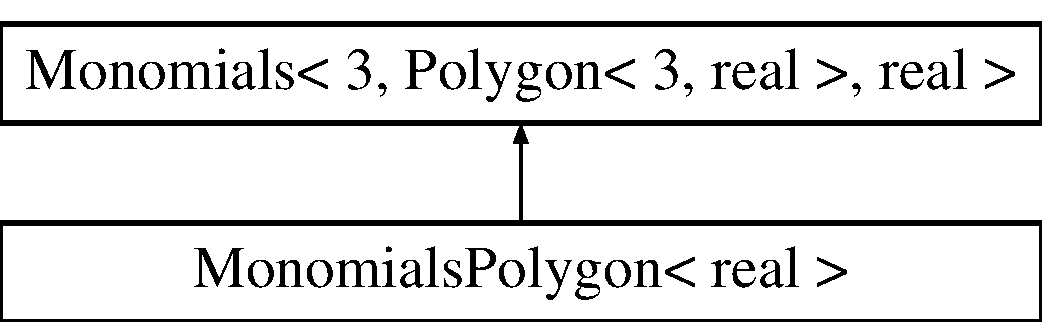
\includegraphics[height=2.000000cm]{class_monomials_polygon}
\end{center}
\end{figure}
\subsection*{Public Member Functions}
\begin{DoxyCompactItemize}
\item 
\hyperlink{class_monomials_polygon_a15ff4c26d8e8948a3233a2cf31cfaccd}{Monomials\+Polygon} (const shared\+\_\+ptr$<$ \hyperlink{class_polygon}{Polygon}$<$ 3, real $>$$>$ \&figure)\hypertarget{class_monomials_polygon_a15ff4c26d8e8948a3233a2cf31cfaccd}{}\label{class_monomials_polygon_a15ff4c26d8e8948a3233a2cf31cfaccd}

\begin{DoxyCompactList}\small\item\em Constructor from \hyperlink{class_polygon}{Polygon}. \end{DoxyCompactList}\item 
real \hyperlink{class_monomials_polygon_a789109ea081ae68f3d2219fc115e7de7}{evaluate} (const \hyperlink{class_point}{Point}$<$ 3, real $>$ \&p, long i)
\begin{DoxyCompactList}\small\item\em Function to evaluate the monomial in a point. \end{DoxyCompactList}\end{DoxyCompactItemize}
\subsection*{Public Attributes}
\begin{DoxyCompactItemize}
\item 
long {\bfseries indexX}\hypertarget{class_monomials_polygon_a67653a8a7045863c5ce2789e327fdcfd}{}\label{class_monomials_polygon_a67653a8a7045863c5ce2789e327fdcfd}

\item 
long {\bfseries indexY}\hypertarget{class_monomials_polygon_a2599e7ba98876d6d1c2e7510e4fc7b34}{}\label{class_monomials_polygon_a2599e7ba98876d6d1c2e7510e4fc7b34}

\item 
long {\bfseries indexZ}\hypertarget{class_monomials_polygon_a2367e9b41cf7615289ac8d30f000e732}{}\label{class_monomials_polygon_a2367e9b41cf7615289ac8d30f000e732}

\item 
\hyperlink{class_point}{Vector}$<$ 3, real $>$ {\bfseries gradientX}\hypertarget{class_monomials_polygon_a0e83af1a5e822260f79c0fb235480bfd}{}\label{class_monomials_polygon_a0e83af1a5e822260f79c0fb235480bfd}

\item 
\hyperlink{class_point}{Vector}$<$ 3, real $>$ {\bfseries gradientY}\hypertarget{class_monomials_polygon_a13406aff842b61fc89f000697eb4b31b}{}\label{class_monomials_polygon_a13406aff842b61fc89f000697eb4b31b}

\end{DoxyCompactItemize}


\subsection{Detailed Description}
\subsubsection*{template$<$typename real$>$\\*
class Monomials\+Polygon$<$ real $>$}

Class similar to Monomial, but used to compute the similar quantities for a \hyperlink{class_polygon}{Polygon} embedded in 3D. 

\subsection{Member Function Documentation}
\index{Monomials\+Polygon@{Monomials\+Polygon}!evaluate@{evaluate}}
\index{evaluate@{evaluate}!Monomials\+Polygon@{Monomials\+Polygon}}
\subsubsection[{\texorpdfstring{evaluate(const Point$<$ 3, real $>$ \&p, long i)}{evaluate(const Point< 3, real > &p, long i)}}]{\setlength{\rightskip}{0pt plus 5cm}template$<$typename real $>$ real {\bf Monomials\+Polygon}$<$ real $>$\+::evaluate (
\begin{DoxyParamCaption}
\item[{const {\bf Point}$<$ 3, real $>$ \&}]{p, }
\item[{long}]{i}
\end{DoxyParamCaption}
)}\hypertarget{class_monomials_polygon_a789109ea081ae68f3d2219fc115e7de7}{}\label{class_monomials_polygon_a789109ea081ae68f3d2219fc115e7de7}


Function to evaluate the monomial in a point. 


\begin{DoxyParams}{Parameters}
{\em point} & \hyperlink{class_point}{Point} in which I want to evaluate the monomial \\
\hline
{\em i} & Coordinate to keep into account (from 0 to 1 in a \hyperlink{class_polygon}{Polygon}). \\
\hline
\end{DoxyParams}


The documentation for this class was generated from the following file\+:\begin{DoxyCompactItemize}
\item 
Monomials\+Polygon.\+h\end{DoxyCompactItemize}

\hypertarget{class_point}{}\section{Point$<$ embedded, real $>$ Class Template Reference}
\label{class_point}\index{Point$<$ embedded, real $>$@{Point$<$ embedded, real $>$}}


Class to store the position of a point.  




{\ttfamily \#include $<$Point.\+h$>$}

Inheritance diagram for Point$<$ embedded, real $>$\+:\begin{figure}[H]
\begin{center}
\leavevmode
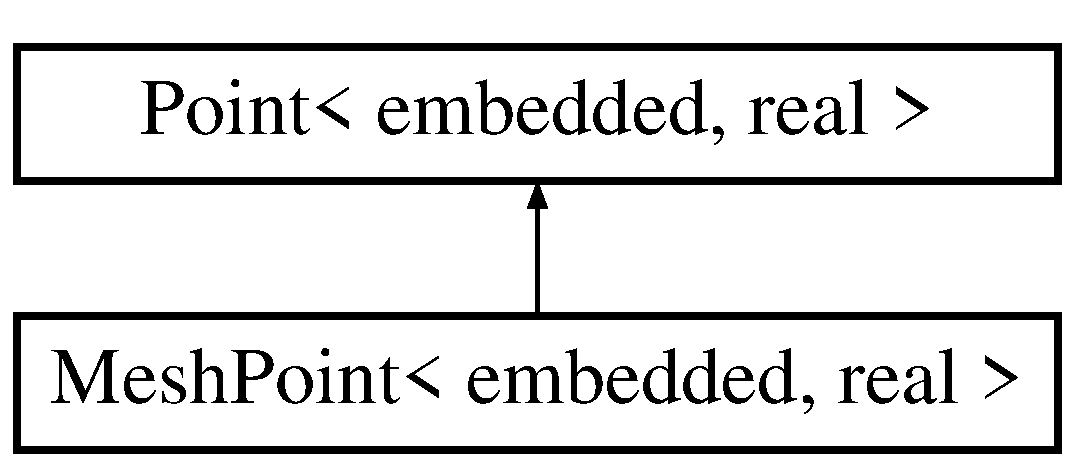
\includegraphics[height=2.000000cm]{class_point}
\end{center}
\end{figure}
\subsection*{Public Member Functions}
\begin{DoxyCompactItemize}
\item 
\hyperlink{class_point_a1dff5286bb0a775c7db78320da11f3d4}{Point} (const array$<$ real, embedded $>$ \&input\+Array)\hypertarget{class_point_a1dff5286bb0a775c7db78320da11f3d4}{}\label{class_point_a1dff5286bb0a775c7db78320da11f3d4}

\begin{DoxyCompactList}\small\item\em Constructor from std\+::array. \end{DoxyCompactList}\item 
\hyperlink{class_point_a5c9c38f9f77cd9089a3a5cadedfee70c}{Point} (const \hyperlink{class_point}{Point}$<$ embedded, real $>$ \&input\+Point)\hypertarget{class_point_a5c9c38f9f77cd9089a3a5cadedfee70c}{}\label{class_point_a5c9c38f9f77cd9089a3a5cadedfee70c}

\begin{DoxyCompactList}\small\item\em Copy constructor. \end{DoxyCompactList}\item 
\hyperlink{class_point_ab4cb590995d17da1537e35f32da3e498}{Point} (const \hyperlink{class_mesh_point}{Mesh\+Point}$<$ embedded, real $>$ \&input\+Point)\hypertarget{class_point_ab4cb590995d17da1537e35f32da3e498}{}\label{class_point_ab4cb590995d17da1537e35f32da3e498}

\begin{DoxyCompactList}\small\item\em Copy constructor from \hyperlink{class_mesh_point}{Mesh\+Point}. \end{DoxyCompactList}\item 
\hyperlink{class_point_ab1a9e6eedb684c43816dc50c586df933}{Point} ()\hypertarget{class_point_ab1a9e6eedb684c43816dc50c586df933}{}\label{class_point_ab1a9e6eedb684c43816dc50c586df933}

\begin{DoxyCompactList}\small\item\em Empty constructor. \end{DoxyCompactList}\item 
{\footnotesize template$<$typename... Args$>$ }\\\hyperlink{class_point_ade059d5c3bf5513c9aaf6bc698f0bb24}{Point} (Args...\+arguments)
\begin{DoxyCompactList}\small\item\em Constructor with variadic template. \end{DoxyCompactList}\item 
long \hyperlink{class_point_a4a87c9a65f2bcd966f1df83a870f117f}{max\+Index} () const \hypertarget{class_point_a4a87c9a65f2bcd966f1df83a870f117f}{}\label{class_point_a4a87c9a65f2bcd966f1df83a870f117f}

\begin{DoxyCompactList}\small\item\em Maximum index of the point. \end{DoxyCompactList}\item 
long \hyperlink{class_point_a5b06a3b1249d1a29e316b00e94522a5a}{max\+Abs\+Index} () const \hypertarget{class_point_a5b06a3b1249d1a29e316b00e94522a5a}{}\label{class_point_a5b06a3b1249d1a29e316b00e94522a5a}

\begin{DoxyCompactList}\small\item\em Maximum index of the point with absolute value. \end{DoxyCompactList}\item 
real \hyperlink{class_point_a885ede7e456888ddb73792df46f88513}{norm} () const \hypertarget{class_point_a885ede7e456888ddb73792df46f88513}{}\label{class_point_a885ede7e456888ddb73792df46f88513}

\begin{DoxyCompactList}\small\item\em L2 norm of the vector. \end{DoxyCompactList}\item 
real \hyperlink{class_point_a6a5c8172bed4fadd3ff4369ac24b627e}{norm\+L1} () const \hypertarget{class_point_a6a5c8172bed4fadd3ff4369ac24b627e}{}\label{class_point_a6a5c8172bed4fadd3ff4369ac24b627e}

\begin{DoxyCompactList}\small\item\em L1 norm of the vector. \end{DoxyCompactList}\item 
string \hyperlink{class_point_a2e471acd2e526217306b148ef5d04d87}{write} () const 
\begin{DoxyCompactList}\small\item\em Output to string. \end{DoxyCompactList}\item 
real \& \hyperlink{class_point_ad9c36be87662ac8b290800ff76b8a3f7}{x} ()\hypertarget{class_point_ad9c36be87662ac8b290800ff76b8a3f7}{}\label{class_point_ad9c36be87662ac8b290800ff76b8a3f7}

\begin{DoxyCompactList}\small\item\em Get the first element by reference. \end{DoxyCompactList}\item 
real \hyperlink{class_point_a155238f2303c1805a976e5ffde2df863}{x} () const \hypertarget{class_point_a155238f2303c1805a976e5ffde2df863}{}\label{class_point_a155238f2303c1805a976e5ffde2df863}

\begin{DoxyCompactList}\small\item\em Get the first element by value. \end{DoxyCompactList}\item 
real \& \hyperlink{class_point_abdedcae417002d4e747b876a346a5062}{y} ()\hypertarget{class_point_abdedcae417002d4e747b876a346a5062}{}\label{class_point_abdedcae417002d4e747b876a346a5062}

\begin{DoxyCompactList}\small\item\em Get the second element by reference. \end{DoxyCompactList}\item 
real \hyperlink{class_point_ad4dc38edfea288dbfed132cf5ce3830a}{y} () const \hypertarget{class_point_ad4dc38edfea288dbfed132cf5ce3830a}{}\label{class_point_ad4dc38edfea288dbfed132cf5ce3830a}

\begin{DoxyCompactList}\small\item\em Get the second element by value. \end{DoxyCompactList}\item 
real \& \hyperlink{class_point_a70f81bbcc60b59191dba261ec8bee87e}{z} ()\hypertarget{class_point_a70f81bbcc60b59191dba261ec8bee87e}{}\label{class_point_a70f81bbcc60b59191dba261ec8bee87e}

\begin{DoxyCompactList}\small\item\em Get the third element by reference. \end{DoxyCompactList}\item 
real \hyperlink{class_point_ae344dd16dddf7ae80f665f085874fd55}{z} () const \hypertarget{class_point_ae344dd16dddf7ae80f665f085874fd55}{}\label{class_point_ae344dd16dddf7ae80f665f085874fd55}

\begin{DoxyCompactList}\small\item\em Get the third element by value. \end{DoxyCompactList}\item 
\hyperlink{class_point}{Point}$<$ embedded, real $>$ \& \hyperlink{class_point_a448799c65927e710a92fcd5b715e3b21}{operator=} (\hyperlink{class_point}{Point}$<$ embedded, real $>$ input\+Point)
\begin{DoxyCompactList}\small\item\em Equal operator. \end{DoxyCompactList}\item 
bool \hyperlink{class_point_a85d75524d6a63f080aca5cec2eca7ec9}{operator==} (const \hyperlink{class_point}{Point}$<$ embedded, real $>$ \&input\+Point) const 
\begin{DoxyCompactList}\small\item\em Check if they are equals. \end{DoxyCompactList}\item 
bool \hyperlink{class_point_af3dfd6f86d375de9c2bd412f9ba31c87}{operator!=} (const \hyperlink{class_point}{Point}$<$ embedded, real $>$ \&input\+Point) const 
\begin{DoxyCompactList}\small\item\em Check if they are different. \end{DoxyCompactList}\item 
real \& \hyperlink{class_point_ab8b7d24713bc91d95cced47933f06198}{operator\mbox{[}$\,$\mbox{]}} (long index)\hypertarget{class_point_ab8b7d24713bc91d95cced47933f06198}{}\label{class_point_ab8b7d24713bc91d95cced47933f06198}

\begin{DoxyCompactList}\small\item\em Get an element by reference. \end{DoxyCompactList}\item 
real \hyperlink{class_point_a6fb29d763d4c786452b071e790db86fc}{operator\mbox{[}$\,$\mbox{]}} (long index) const \hypertarget{class_point_a6fb29d763d4c786452b071e790db86fc}{}\label{class_point_a6fb29d763d4c786452b071e790db86fc}

\begin{DoxyCompactList}\small\item\em Get an element by value. \end{DoxyCompactList}\end{DoxyCompactItemize}
\subsection*{Protected Attributes}
\begin{DoxyCompactItemize}
\item 
array$<$ real, embedded $>$ \hyperlink{class_point_a24b16f288c9f98da13e4719b6ed462e6}{coordinates}\hypertarget{class_point_a24b16f288c9f98da13e4719b6ed462e6}{}\label{class_point_a24b16f288c9f98da13e4719b6ed462e6}

\begin{DoxyCompactList}\small\item\em It stores the coordinates of the point. \end{DoxyCompactList}\end{DoxyCompactItemize}
\subsection*{Friends}
\begin{DoxyCompactItemize}
\item 
{\footnotesize template$<$long embedded2, typename real2 $>$ }\\ostream \& \hyperlink{class_point_ac6eecb3c92e49e305452771a073acf4c}{operator$<$$<$} (ostream \&os, const \hyperlink{class_point}{Point}$<$ embedded2, real2 $>$ \&point)\hypertarget{class_point_ac6eecb3c92e49e305452771a073acf4c}{}\label{class_point_ac6eecb3c92e49e305452771a073acf4c}

\begin{DoxyCompactList}\small\item\em Output operator. \end{DoxyCompactList}\item 
{\footnotesize template$<$long embedded2, typename real2 $>$ }\\\hyperlink{class_point}{Point}$<$ embedded2, real2 $>$ \hyperlink{class_point_a3ea6134b47e84bd4452443ffde47e70f}{operator+} (const \hyperlink{class_point}{Point}$<$ embedded2, real2 $>$ \&point1, const \hyperlink{class_point}{Point}$<$ embedded2, real2 $>$ \&point2)\hypertarget{class_point_a3ea6134b47e84bd4452443ffde47e70f}{}\label{class_point_a3ea6134b47e84bd4452443ffde47e70f}

\begin{DoxyCompactList}\small\item\em Sum operator. \end{DoxyCompactList}\item 
{\footnotesize template$<$long embedded2, typename real2 $>$ }\\\hyperlink{class_point}{Point}$<$ embedded2, real2 $>$ \hyperlink{class_point_ab65b17238ecddcc87348a5e9c55892f3}{operator-\/} (const \hyperlink{class_point}{Point}$<$ embedded2, real2 $>$ \&point1, const \hyperlink{class_point}{Point}$<$ embedded2, real2 $>$ \&point2)\hypertarget{class_point_ab65b17238ecddcc87348a5e9c55892f3}{}\label{class_point_ab65b17238ecddcc87348a5e9c55892f3}

\begin{DoxyCompactList}\small\item\em Difference operator. \end{DoxyCompactList}\item 
{\footnotesize template$<$long embedded2, typename real2 $>$ }\\\hyperlink{class_point}{Point}$<$ embedded2, real2 $>$ \hyperlink{class_point_aadb04db36a16719114875b8a267ca639}{operator-\/} (const \hyperlink{class_point}{Point}$<$ embedded2, real2 $>$ \&point1)\hypertarget{class_point_aadb04db36a16719114875b8a267ca639}{}\label{class_point_aadb04db36a16719114875b8a267ca639}

\begin{DoxyCompactList}\small\item\em Difference operator. \end{DoxyCompactList}\item 
{\footnotesize template$<$long embedded2, typename real2 $>$ }\\real2 \hyperlink{class_point_afc1da372540656b24f224e7959624c08}{operator$\ast$} (const \hyperlink{class_point}{Point}$<$ embedded2, real2 $>$ \&point1, const \hyperlink{class_point}{Point}$<$ embedded2, real2 $>$ \&point2)\hypertarget{class_point_afc1da372540656b24f224e7959624c08}{}\label{class_point_afc1da372540656b24f224e7959624c08}

\begin{DoxyCompactList}\small\item\em Product operator. \end{DoxyCompactList}\item 
{\footnotesize template$<$long embedded2, typename real2 $>$ }\\\hyperlink{class_point}{Point}$<$ embedded2, real2 $>$ \hyperlink{class_point_acaaff0a0864728144ee00bb8772dfd74}{operator$\ast$} (long double coefficient, const \hyperlink{class_point}{Point}$<$ embedded2, real2 $>$ \&point)\hypertarget{class_point_acaaff0a0864728144ee00bb8772dfd74}{}\label{class_point_acaaff0a0864728144ee00bb8772dfd74}

\begin{DoxyCompactList}\small\item\em Product operator. \end{DoxyCompactList}\item 
{\footnotesize template$<$long embedded2, typename real2 $>$ }\\\hyperlink{class_point}{Point}$<$ embedded2, real2 $>$ \hyperlink{class_point_ab2682a3fd01359b9a694b8f8494341e1}{operator$\ast$} (const \hyperlink{class_point}{Point}$<$ embedded2, real2 $>$ \&point, long double coefficient)\hypertarget{class_point_ab2682a3fd01359b9a694b8f8494341e1}{}\label{class_point_ab2682a3fd01359b9a694b8f8494341e1}

\begin{DoxyCompactList}\small\item\em Product operator. \end{DoxyCompactList}\item 
{\footnotesize template$<$long embedded2, typename real2 $>$ }\\\hyperlink{class_point}{Point}$<$ embedded2, real2 $>$ \hyperlink{class_point_a587faaadac82c79e9119d8bc59396c79}{operator/} (const \hyperlink{class_point}{Point}$<$ embedded2, real2 $>$ \&point, long double coefficient)\hypertarget{class_point_a587faaadac82c79e9119d8bc59396c79}{}\label{class_point_a587faaadac82c79e9119d8bc59396c79}

\begin{DoxyCompactList}\small\item\em Dividing operator. \end{DoxyCompactList}\item 
{\footnotesize template$<$long embedded2, typename real2 $>$ }\\\hyperlink{class_point}{Point}$<$ embedded2, real2 $>$ \hyperlink{class_point_a951dd5bf519f7daabc4ba4e61657cc26}{cross} (const \hyperlink{class_point}{Point}$<$ embedded2, real2 $>$ \&point1, const \hyperlink{class_point}{Point}$<$ embedded2, real2 $>$ \&point2)
\begin{DoxyCompactList}\small\item\em Cross product of 2 vector. \end{DoxyCompactList}\item 
{\footnotesize template$<$long embedded2, typename real2 $>$ }\\\hyperlink{class_point}{Point}$<$ embedded2, real2 $>$ \hyperlink{class_point_a94ebaad0db80d547a452cba37e98e1ca}{prod\+Term\+By\+Term} (const \hyperlink{class_point}{Point}$<$ embedded2, real2 $>$ \&point1, const \hyperlink{class_point}{Point}$<$ embedded2, real2 $>$ \&point2)
\begin{DoxyCompactList}\small\item\em Product term by term. \end{DoxyCompactList}\end{DoxyCompactItemize}


\subsection{Detailed Description}
\subsubsection*{template$<$long embedded, typename real = double$>$\\*
class Point$<$ embedded, real $>$}

Class to store the position of a point. 

Virtually any dimensions allowed. Some methods are available only for d=2 or d=3. Any vector can be seen as a point. Some appropriate typedef (Vector2D, Vector3D, Vector$<$embedded$>$, Vector$<$embedded,real$>$) are implemented. 

\subsection{Constructor \& Destructor Documentation}
\index{Point@{Point}!Point@{Point}}
\index{Point@{Point}!Point@{Point}}
\subsubsection[{\texorpdfstring{Point(\+Args...\+arguments)}{Point(Args...arguments)}}]{\setlength{\rightskip}{0pt plus 5cm}template$<$long embedded, typename real = double$>$ template$<$typename... Args$>$ {\bf Point}$<$ embedded, real $>$\+::{\bf Point} (
\begin{DoxyParamCaption}
\item[{Args...}]{arguments}
\end{DoxyParamCaption}
)\hspace{0.3cm}{\ttfamily [inline]}}\hypertarget{class_point_ade059d5c3bf5513c9aaf6bc698f0bb24}{}\label{class_point_ade059d5c3bf5513c9aaf6bc698f0bb24}


Constructor with variadic template. 

Source\+: \href{http://stackoverflow.com/questions/8158261/templates-how-to-control-number-of-constructor-args-using-template-variable}{\tt http\+://stackoverflow.\+com/questions/8158261/templates-\/how-\/to-\/control-\/number-\/of-\/constructor-\/args-\/using-\/template-\/variable} 

\subsection{Member Function Documentation}
\index{Point@{Point}!operator"!=@{operator"!=}}
\index{operator"!=@{operator"!=}!Point@{Point}}
\subsubsection[{\texorpdfstring{operator"!=(const Point$<$ embedded, real $>$ \&input\+Point) const }{operator!=(const Point< embedded, real > &inputPoint) const }}]{\setlength{\rightskip}{0pt plus 5cm}template$<$long embedded, typename real$>$ bool {\bf Point}$<$ embedded, real $>$\+::operator!= (
\begin{DoxyParamCaption}
\item[{const {\bf Point}$<$ embedded, real $>$ \&}]{input\+Point}
\end{DoxyParamCaption}
) const}\hypertarget{class_point_af3dfd6f86d375de9c2bd412f9ba31c87}{}\label{class_point_af3dfd6f86d375de9c2bd412f9ba31c87}


Check if they are different. 

It compares only coordinates \index{Point@{Point}!operator=@{operator=}}
\index{operator=@{operator=}!Point@{Point}}
\subsubsection[{\texorpdfstring{operator=(\+Point$<$ embedded, real $>$ input\+Point)}{operator=(Point< embedded, real > inputPoint)}}]{\setlength{\rightskip}{0pt plus 5cm}template$<$long embedded, typename real$>$ {\bf Point}$<$ embedded, real $>$ \& {\bf Point}$<$ embedded, real $>$\+::operator= (
\begin{DoxyParamCaption}
\item[{{\bf Point}$<$ embedded, real $>$}]{input\+Point}
\end{DoxyParamCaption}
)}\hypertarget{class_point_a448799c65927e710a92fcd5b715e3b21}{}\label{class_point_a448799c65927e710a92fcd5b715e3b21}


Equal operator. 

Be careful, it copies only the coordinates, not the other things \index{Point@{Point}!operator==@{operator==}}
\index{operator==@{operator==}!Point@{Point}}
\subsubsection[{\texorpdfstring{operator==(const Point$<$ embedded, real $>$ \&input\+Point) const }{operator==(const Point< embedded, real > &inputPoint) const }}]{\setlength{\rightskip}{0pt plus 5cm}template$<$long embedded, typename real$>$ bool {\bf Point}$<$ embedded, real $>$\+::operator== (
\begin{DoxyParamCaption}
\item[{const {\bf Point}$<$ embedded, real $>$ \&}]{input\+Point}
\end{DoxyParamCaption}
) const}\hypertarget{class_point_a85d75524d6a63f080aca5cec2eca7ec9}{}\label{class_point_a85d75524d6a63f080aca5cec2eca7ec9}


Check if they are equals. 

It compares only coordinates \index{Point@{Point}!write@{write}}
\index{write@{write}!Point@{Point}}
\subsubsection[{\texorpdfstring{write() const }{write() const }}]{\setlength{\rightskip}{0pt plus 5cm}template$<$long embedded, typename real $>$ string {\bf Point}$<$ embedded, real $>$\+::write (
\begin{DoxyParamCaption}
{}
\end{DoxyParamCaption}
) const}\hypertarget{class_point_a2e471acd2e526217306b148ef5d04d87}{}\label{class_point_a2e471acd2e526217306b148ef5d04d87}


Output to string. 

\begin{DoxyReturn}{Returns}
std\+::string representing the \hyperlink{class_point}{Point} 
\end{DoxyReturn}


\subsection{Friends And Related Function Documentation}
\index{Point@{Point}!cross@{cross}}
\index{cross@{cross}!Point@{Point}}
\subsubsection[{\texorpdfstring{cross}{cross}}]{\setlength{\rightskip}{0pt plus 5cm}template$<$long embedded, typename real = double$>$ template$<$long embedded2, typename real2 $>$ {\bf Point}$<$embedded2,real2$>$ cross (
\begin{DoxyParamCaption}
\item[{const {\bf Point}$<$ embedded2, real2 $>$ \&}]{point1, }
\item[{const {\bf Point}$<$ embedded2, real2 $>$ \&}]{point2}
\end{DoxyParamCaption}
)\hspace{0.3cm}{\ttfamily [friend]}}\hypertarget{class_point_a951dd5bf519f7daabc4ba4e61657cc26}{}\label{class_point_a951dd5bf519f7daabc4ba4e61657cc26}


Cross product of 2 vector. 

\begin{DoxyReturn}{Returns}
The resulting vector of the cross product Here \hyperlink{class_point}{Point} is intended as Vector. Cross product keeping sign into consideration 
\end{DoxyReturn}
\index{Point@{Point}!prod\+Term\+By\+Term@{prod\+Term\+By\+Term}}
\index{prod\+Term\+By\+Term@{prod\+Term\+By\+Term}!Point@{Point}}
\subsubsection[{\texorpdfstring{prod\+Term\+By\+Term}{prodTermByTerm}}]{\setlength{\rightskip}{0pt plus 5cm}template$<$long embedded, typename real = double$>$ template$<$long embedded2, typename real2 $>$ {\bf Point}$<$embedded2,real2$>$ prod\+Term\+By\+Term (
\begin{DoxyParamCaption}
\item[{const {\bf Point}$<$ embedded2, real2 $>$ \&}]{point1, }
\item[{const {\bf Point}$<$ embedded2, real2 $>$ \&}]{point2}
\end{DoxyParamCaption}
)\hspace{0.3cm}{\ttfamily [friend]}}\hypertarget{class_point_a94ebaad0db80d547a452cba37e98e1ca}{}\label{class_point_a94ebaad0db80d547a452cba37e98e1ca}


Product term by term. 

\begin{DoxyReturn}{Returns}
A point with component i being the product of the i components of the 2 vectors 
\end{DoxyReturn}


The documentation for this class was generated from the following files\+:\begin{DoxyCompactItemize}
\item 
Mesh\+Point.\+h\item 
Point.\+h\end{DoxyCompactItemize}

\hypertarget{class_polygon}{}\section{Polygon$<$ embedded, real $>$ Class Template Reference}
\label{class_polygon}\index{Polygon$<$ embedded, real $>$@{Polygon$<$ embedded, real $>$}}


Class to represent a \hyperlink{class_polygon}{Polygon} in a \hyperlink{class_mesh}{Mesh}, embedded in 2D or 3D.  




{\ttfamily \#include $<$Polygon.\+h$>$}

Inheritance diagram for Polygon$<$ embedded, real $>$\+:\begin{figure}[H]
\begin{center}
\leavevmode
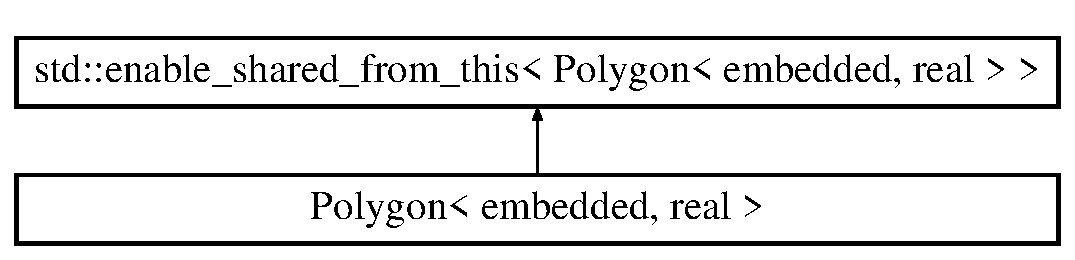
\includegraphics[height=2.000000cm]{class_polygon}
\end{center}
\end{figure}
\subsection*{Public Member Functions}
\begin{DoxyCompactItemize}
\item 
\hyperlink{class_polygon_af5bca80e9a6a306460d7235cd5436385}{Polygon} (const private\+Struct \&, const vector$<$ shared\+\_\+ptr$<$ \hyperlink{class_mesh_point}{Mesh\+Point}$<$ embedded, real $>$$>$$>$ \&vertex\+Vector)
\begin{DoxyCompactList}\small\item\em Constructor from a vector of shared\+\_\+ptr. \end{DoxyCompactList}\item 
\hyperlink{class_polygon_a13a8d5ce1ddba0c542fdbb667b0a9cc9}{Polygon} (const private\+Struct \&)
\begin{DoxyCompactList}\small\item\em Empty constructor. \end{DoxyCompactList}\item 
{\footnotesize template$<$typename... Args$>$ }\\\hyperlink{class_polygon_aeeae92fe9691e9bba131228f38ac08a7}{Polygon} (const private\+Struct \&, Args...\+arguments)
\begin{DoxyCompactList}\small\item\em Constructor with variadic template. \end{DoxyCompactList}\item 
void \hyperlink{class_polygon_af227451b2f12b89bab30c619f3805d97}{add\+Point} (const shared\+\_\+ptr$<$ \hyperlink{class_mesh_point}{Mesh\+Point}$<$ embedded, real $>$$>$ \&p1)\hypertarget{class_polygon_af227451b2f12b89bab30c619f3805d97}{}\label{class_polygon_af227451b2f12b89bab30c619f3805d97}

\begin{DoxyCompactList}\small\item\em Add a new vertex to the \hyperlink{class_polygon}{Polygon}. \end{DoxyCompactList}\item 
void \hyperlink{class_polygon_a663e3901b49a938202abc2ac89d963df}{add\+Polyhedron} (weak\+\_\+ptr$<$ \hyperlink{class_polyhedron}{Polyhedron}$<$ embedded, real $>$$>$ \hyperlink{class_polygon_a57bfc8000b2c43678fcc5841252f744d}{polyhedron})\hypertarget{class_polygon_a663e3901b49a938202abc2ac89d963df}{}\label{class_polygon_a663e3901b49a938202abc2ac89d963df}

\begin{DoxyCompactList}\small\item\em Add a new \hyperlink{class_polyhedron}{Polyhedron} having this as face. \end{DoxyCompactList}\item 
\hyperlink{class_point}{Vector}$<$ embedded, real $>$ {\bfseries compute\+Centroid} ()\hypertarget{class_polygon_a53555fe6109d8ddf75d432f157f021c7}{}\label{class_polygon_a53555fe6109d8ddf75d432f157f021c7}

\item 
real {\bfseries compute\+Area} ()\hypertarget{class_polygon_af53fc15da94e704d6aab016171f6c15f}{}\label{class_polygon_af53fc15da94e704d6aab016171f6c15f}

\item 
real {\bfseries get\+Diameter} ()\hypertarget{class_polygon_a3b375cd2abd0f7535041b17d7d7b4f14}{}\label{class_polygon_a3b375cd2abd0f7535041b17d7d7b4f14}

\item 
real \hyperlink{class_polygon_a96f0c55cdb99e0cfc87ecf4d855c91d3}{h\+Triangle} ()\hypertarget{class_polygon_a96f0c55cdb99e0cfc87ecf4d855c91d3}{}\label{class_polygon_a96f0c55cdb99e0cfc87ecf4d855c91d3}

\begin{DoxyCompactList}\small\item\em Compute the maximum distance between 2 vertexes. Necessary for the paramether h of the \hyperlink{class_mesh}{Mesh}. \end{DoxyCompactList}\item 
void {\bfseries initialize} ()\hypertarget{class_polygon_a3d0aa945fd528d2c6ee44838f9eaad6f}{}\label{class_polygon_a3d0aa945fd528d2c6ee44838f9eaad6f}

\item 
bool {\bfseries is\+Conflict\+Point} (\hyperlink{class_point}{Point}$<$ embedded, real $>$ \&\hyperlink{class_polygon_a56f83109c9c8ad214f41bd8036efb32c}{point})\hypertarget{class_polygon_a4df44a07db58dba116ae2362fb08e9aa}{}\label{class_polygon_a4df44a07db58dba116ae2362fb08e9aa}

\item 
shared\+\_\+ptr$<$ \hyperlink{class_mesh_point}{Mesh\+Point}$<$ embedded, real $>$ $>$ \hyperlink{class_polygon_a10ed15053764f6170fee5b4f06a76174}{is\+Point\+A\+Vertex} (\hyperlink{class_point}{Point}$<$ embedded, real $>$ \&\hyperlink{class_polygon_a56f83109c9c8ad214f41bd8036efb32c}{point})\hypertarget{class_polygon_a10ed15053764f6170fee5b4f06a76174}{}\label{class_polygon_a10ed15053764f6170fee5b4f06a76174}

\begin{DoxyCompactList}\small\item\em Given a simple \hyperlink{class_point}{Point} return if the \hyperlink{class_point}{Point} coincides with a vertex. \end{DoxyCompactList}\item 
bool {\bfseries is\+Point\+Inside} (\hyperlink{class_point}{Point}$<$ embedded, real $>$ \&\hyperlink{class_polygon_a56f83109c9c8ad214f41bd8036efb32c}{point})\hypertarget{class_polygon_a36fa14ce6d01941d406a04c795c2742d}{}\label{class_polygon_a36fa14ce6d01941d406a04c795c2742d}

\item 
array$<$ shared\+\_\+ptr$<$ \hyperlink{class_mesh_point}{Mesh\+Point}$<$ embedded, real $>$ $>$, 2 $>$ {\bfseries is\+Point\+On\+Boundary} (\hyperlink{class_point}{Point}$<$ embedded, real $>$ \&\hyperlink{class_polygon_a56f83109c9c8ad214f41bd8036efb32c}{point})\hypertarget{class_polygon_a6462af95446a3bd604146e10ff358860}{}\label{class_polygon_a6462af95446a3bd604146e10ff358860}

\item 
\hyperlink{class_point}{Vector}$<$ 3, real $>$ \hyperlink{class_polygon_aa12bdc3f0990036909241a3294ca90ae}{compute\+Normal} ()
\begin{DoxyCompactList}\small\item\em Normal computed with Newell\textquotesingle{}s algorithm. \end{DoxyCompactList}\item 
void {\bfseries shrink\+\_\+to\+\_\+fit} ()\hypertarget{class_polygon_af63fd7046132c422a90c52c3fc092cb3}{}\label{class_polygon_af63fd7046132c422a90c52c3fc092cb3}

\item 
real \hyperlink{class_polygon_ae119dd09d659fc1255fcfa1c45659a51}{space} ()
\begin{DoxyCompactList}\small\item\em Area of the \hyperlink{class_polygon}{Polygon}. \end{DoxyCompactList}\item 
void \hyperlink{class_polygon_aad5a195054aa08f073e59ea907bd5d60}{switch\+Points\+Order} ()\hypertarget{class_polygon_aad5a195054aa08f073e59ea907bd5d60}{}\label{class_polygon_aad5a195054aa08f073e59ea907bd5d60}

\begin{DoxyCompactList}\small\item\em Invert the orientation of the \hyperlink{class_polygon}{Polygon}. \end{DoxyCompactList}\item 
string \hyperlink{class_polygon_ac36032b05bfac321af17c5992de2deae}{write} ()
\begin{DoxyCompactList}\small\item\em Output to string. \end{DoxyCompactList}\item 
bool {\bfseries get\+Is\+Boundary} () const \hypertarget{class_polygon_a25bd0bca4495328793bdf0938bc26e1b}{}\label{class_polygon_a25bd0bca4495328793bdf0938bc26e1b}

\item 
void {\bfseries set\+Is\+Boundary} (bool input\+Is\+Boundary)\hypertarget{class_polygon_ab1dd3c0dbe875da0e34e16e4b37f8ab0}{}\label{class_polygon_ab1dd3c0dbe875da0e34e16e4b37f8ab0}

\item 
long {\bfseries number\+Of\+Polyhedrons} () const \hypertarget{class_polygon_ac5c64f6a2369301bf7f542c0543798f0}{}\label{class_polygon_ac5c64f6a2369301bf7f542c0543798f0}

\item 
real {\bfseries get\+Area} () const \hypertarget{class_polygon_a12cd12e47dd6b7d7ea0fd7fb10db4eed}{}\label{class_polygon_a12cd12e47dd6b7d7ea0fd7fb10db4eed}

\item 
const \hyperlink{class_point}{Vector}$<$ 3, real $>$ \& {\bfseries get\+Normal} () const \hypertarget{class_polygon_a3c6b41daa52625ae8fc00517b4876032}{}\label{class_polygon_a3c6b41daa52625ae8fc00517b4876032}

\item 
const \hyperlink{class_point}{Point}$<$ embedded, real $>$ \& {\bfseries get\+Centroid} () const \hypertarget{class_polygon_a8e4e62c641a9b6bee472d0e066680e08}{}\label{class_polygon_a8e4e62c641a9b6bee472d0e066680e08}

\item 
const shared\+\_\+ptr$<$ \hyperlink{class_mesh_point}{Mesh\+Point}$<$ embedded, real $>$ $>$ \& \hyperlink{class_polygon_a56f83109c9c8ad214f41bd8036efb32c}{point} (long index)\hypertarget{class_polygon_a56f83109c9c8ad214f41bd8036efb32c}{}\label{class_polygon_a56f83109c9c8ad214f41bd8036efb32c}

\begin{DoxyCompactList}\small\item\em Get a shared pointer to a \hyperlink{class_point}{Point} in point\+Vector. \end{DoxyCompactList}\item 
const weak\+\_\+ptr$<$ \hyperlink{class_polyhedron}{Polyhedron}$<$ embedded, real $>$ $>$ \& \hyperlink{class_polygon_a57bfc8000b2c43678fcc5841252f744d}{polyhedron} (long index)\hypertarget{class_polygon_a57bfc8000b2c43678fcc5841252f744d}{}\label{class_polygon_a57bfc8000b2c43678fcc5841252f744d}

\begin{DoxyCompactList}\small\item\em Get a weak pointer to a \hyperlink{class_polyhedron}{Polyhedron} in polyhedron\+Vector. \end{DoxyCompactList}\item 
shared\+\_\+ptr$<$ \hyperlink{class_mesh_point}{Mesh\+Point}$<$ embedded, real $>$ $>$ \hyperlink{class_polygon_aeca77478436766b314a6dee946f28ad4}{operator\mbox{[}$\,$\mbox{]}} (long index)\hypertarget{class_polygon_aeca77478436766b314a6dee946f28ad4}{}\label{class_polygon_aeca77478436766b314a6dee946f28ad4}

\begin{DoxyCompactList}\small\item\em Get the \hyperlink{class_mesh_point}{Mesh\+Point} with a particular index. \end{DoxyCompactList}\item 
bool \hyperlink{class_polygon_aba500dd40a805acea4bf7c050b6ba95a}{operator==} (const \hyperlink{class_polygon}{Polygon}$<$ embedded, real $>$ \&polygon)\hypertarget{class_polygon_aba500dd40a805acea4bf7c050b6ba95a}{}\label{class_polygon_aba500dd40a805acea4bf7c050b6ba95a}

\begin{DoxyCompactList}\small\item\em Check if equal operator. \end{DoxyCompactList}\item 
bool \hyperlink{class_polygon_abf1bf0edcebc33c975d81a704904ae0e}{operator!=} (const \hyperlink{class_polygon}{Polygon}$<$ embedded, real $>$ \&polygon)\hypertarget{class_polygon_abf1bf0edcebc33c975d81a704904ae0e}{}\label{class_polygon_abf1bf0edcebc33c975d81a704904ae0e}

\begin{DoxyCompactList}\small\item\em Check if different operator. \end{DoxyCompactList}\end{DoxyCompactItemize}
\subsection*{Static Public Member Functions}
\begin{DoxyCompactItemize}
\item 
{\footnotesize template$<$typename... Args$>$ }\\static shared\+\_\+ptr$<$ \hyperlink{class_polygon}{Polygon}$<$ embedded, real $>$ $>$ \hyperlink{class_polygon_a2eb322f57f8043dfb195f3514b8b11e7}{make\+\_\+shared\+\_\+\+Polygon} (Args...\+arguments)
\begin{DoxyCompactList}\small\item\em The {\bfseries only} constructor for \hyperlink{class_polygon}{Polygon}. \end{DoxyCompactList}\end{DoxyCompactItemize}
\subsection*{Public Attributes}
\begin{DoxyCompactItemize}
\item 
long \hyperlink{class_polygon_a84d5ff2931fc01477beb2acc4c7448fb}{number\+Of\+Points}
\end{DoxyCompactItemize}
\subsection*{Protected Attributes}
\begin{DoxyCompactItemize}
\item 
vector$<$ shared\+\_\+ptr$<$ \hyperlink{class_mesh_point}{Mesh\+Point}$<$ embedded, real $>$ $>$ $>$ \hyperlink{class_polygon_a5869c5a0ffefb4afb44509fd9c611e7c}{point\+Vector}\hypertarget{class_polygon_a5869c5a0ffefb4afb44509fd9c611e7c}{}\label{class_polygon_a5869c5a0ffefb4afb44509fd9c611e7c}

\begin{DoxyCompactList}\small\item\em Vector of {\bfseries ordered} vertexes. \end{DoxyCompactList}\item 
bool \hyperlink{class_polygon_ac1f76ec494bfecbb4336ee908391d392}{is\+Boundary}\hypertarget{class_polygon_ac1f76ec494bfecbb4336ee908391d392}{}\label{class_polygon_ac1f76ec494bfecbb4336ee908391d392}

\begin{DoxyCompactList}\small\item\em Tells if the \hyperlink{class_polygon}{Polygon} is on the boundary. \end{DoxyCompactList}\item 
real \hyperlink{class_polygon_a97237c3271514d911648c249b3078842}{area}
\item 
\hyperlink{class_point}{Vector}$<$ 3, real $>$ \hyperlink{class_polygon_a23acd35ab3af1494250f68fe733f2a1c}{normal}
\item 
\hyperlink{class_point}{Point}$<$ embedded, real $>$ \hyperlink{class_polygon_a26dc4392a659ca45b70410260e7c890d}{centroid}
\item 
vector$<$ weak\+\_\+ptr$<$ \hyperlink{class_polyhedron}{Polyhedron}$<$ embedded, real $>$ $>$ $>$ \hyperlink{class_polygon_aac6777656621ccf17a4a6f144000cd56}{polyhedron\+Vector}
\begin{DoxyCompactList}\small\item\em Vector of Polyhedrons with this \hyperlink{class_polygon}{Polygon} as face. \end{DoxyCompactList}\end{DoxyCompactItemize}
\subsection*{Friends}
\begin{DoxyCompactItemize}
\item 
{\footnotesize template$<$long embedded2, typename real2 $>$ }\\ostream \& \hyperlink{class_polygon_a8261423e708f9f7c67f05e09fd5aff85}{operator$<$$<$} (ostream \&os, const \hyperlink{class_polygon}{Polygon}$<$ embedded2, real2 $>$ \&polygon)\hypertarget{class_polygon_a8261423e708f9f7c67f05e09fd5aff85}{}\label{class_polygon_a8261423e708f9f7c67f05e09fd5aff85}

\begin{DoxyCompactList}\small\item\em Output operator. \end{DoxyCompactList}\end{DoxyCompactItemize}


\subsection{Detailed Description}
\subsubsection*{template$<$long embedded, typename real = double$>$\\*
class Polygon$<$ embedded, real $>$}

Class to represent a \hyperlink{class_polygon}{Polygon} in a \hyperlink{class_mesh}{Mesh}, embedded in 2D or 3D. 

It can be an element of the \hyperlink{class_mesh}{Mesh} in 2D, or a face of a \hyperlink{class_polyhedron}{Polyhedron} in 3D. The only way to initialize it is to call make\+\_\+shared\+\_\+\+Polygon Area, normal and centroid are computed during initialization and saved. Inheritance from enable\+\_\+shared\+\_\+from\+\_\+this to obtain a shared\+\_\+ptr from this. 

\subsection{Constructor \& Destructor Documentation}
\index{Polygon@{Polygon}!Polygon@{Polygon}}
\index{Polygon@{Polygon}!Polygon@{Polygon}}
\subsubsection[{\texorpdfstring{Polygon(const private\+Struct \&, const vector$<$ shared\+\_\+ptr$<$ Mesh\+Point$<$ embedded, real $>$$>$$>$ \&vertex\+Vector)}{Polygon(const privateStruct &, const vector< shared_ptr< MeshPoint< embedded, real >>> &vertexVector)}}]{\setlength{\rightskip}{0pt plus 5cm}template$<$long embedded, typename real $>$ {\bf Polygon}$<$ embedded, real $>$\+::{\bf Polygon} (
\begin{DoxyParamCaption}
\item[{const private\+Struct \&}]{, }
\item[{const vector$<$ shared\+\_\+ptr$<$ {\bf Mesh\+Point}$<$ embedded, real $>$$>$$>$ \&}]{vertex\+Vector}
\end{DoxyParamCaption}
)}\hypertarget{class_polygon_af5bca80e9a6a306460d7235cd5436385}{}\label{class_polygon_af5bca80e9a6a306460d7235cd5436385}


Constructor from a vector of shared\+\_\+ptr. 

DO N\+OT U\+SE.

Called by make\+\_\+shared\+\_\+\+Polygon \index{Polygon@{Polygon}!Polygon@{Polygon}}
\index{Polygon@{Polygon}!Polygon@{Polygon}}
\subsubsection[{\texorpdfstring{Polygon(const private\+Struct \&)}{Polygon(const privateStruct &)}}]{\setlength{\rightskip}{0pt plus 5cm}template$<$long embedded, typename real = double$>$ {\bf Polygon}$<$ embedded, real $>$\+::{\bf Polygon} (
\begin{DoxyParamCaption}
\item[{const private\+Struct \&}]{}
\end{DoxyParamCaption}
)\hspace{0.3cm}{\ttfamily [inline]}}\hypertarget{class_polygon_a13a8d5ce1ddba0c542fdbb667b0a9cc9}{}\label{class_polygon_a13a8d5ce1ddba0c542fdbb667b0a9cc9}


Empty constructor. 

DO N\+OT U\+SE.

Called by make\+\_\+shared\+\_\+\+Polygon \index{Polygon@{Polygon}!Polygon@{Polygon}}
\index{Polygon@{Polygon}!Polygon@{Polygon}}
\subsubsection[{\texorpdfstring{Polygon(const private\+Struct \&, Args...\+arguments)}{Polygon(const privateStruct &, Args...arguments)}}]{\setlength{\rightskip}{0pt plus 5cm}template$<$long embedded, typename real = double$>$ template$<$typename... Args$>$ {\bf Polygon}$<$ embedded, real $>$\+::{\bf Polygon} (
\begin{DoxyParamCaption}
\item[{const private\+Struct \&}]{, }
\item[{Args...}]{arguments}
\end{DoxyParamCaption}
)\hspace{0.3cm}{\ttfamily [inline]}}\hypertarget{class_polygon_aeeae92fe9691e9bba131228f38ac08a7}{}\label{class_polygon_aeeae92fe9691e9bba131228f38ac08a7}


Constructor with variadic template. 

DO N\+OT U\+SE.

Source\+: \href{http://stackoverflow.com/questions/8158261/templates-how-to-control-number-of-constructor-args-using-template-variable}{\tt http\+://stackoverflow.\+com/questions/8158261/templates-\/how-\/to-\/control-\/number-\/of-\/constructor-\/args-\/using-\/template-\/variable} Called by make\+\_\+shared\+\_\+\+Polygon 

\subsection{Member Function Documentation}
\index{Polygon@{Polygon}!compute\+Normal@{compute\+Normal}}
\index{compute\+Normal@{compute\+Normal}!Polygon@{Polygon}}
\subsubsection[{\texorpdfstring{compute\+Normal()}{computeNormal()}}]{\setlength{\rightskip}{0pt plus 5cm}template$<$long embedded, typename real $>$ {\bf Vector}$<$ 3, real $>$ {\bf Polygon}$<$ embedded, real $>$\+::compute\+Normal (
\begin{DoxyParamCaption}
{}
\end{DoxyParamCaption}
)}\hypertarget{class_polygon_aa12bdc3f0990036909241a3294ca90ae}{}\label{class_polygon_aa12bdc3f0990036909241a3294ca90ae}


Normal computed with Newell\textquotesingle{}s algorithm. 

Source\+: \href{http://www.gamedev.net/topic/416131-calculating-a-polygon-normal/?p=3771628}{\tt http\+://www.\+gamedev.\+net/topic/416131-\/calculating-\/a-\/polygon-\/normal/?p=3771628} \index{Polygon@{Polygon}!make\+\_\+shared\+\_\+\+Polygon@{make\+\_\+shared\+\_\+\+Polygon}}
\index{make\+\_\+shared\+\_\+\+Polygon@{make\+\_\+shared\+\_\+\+Polygon}!Polygon@{Polygon}}
\subsubsection[{\texorpdfstring{make\+\_\+shared\+\_\+\+Polygon(\+Args...\+arguments)}{make_shared_Polygon(Args...arguments)}}]{\setlength{\rightskip}{0pt plus 5cm}template$<$long embedded, typename real = double$>$ template$<$typename... Args$>$ static shared\+\_\+ptr$<${\bf Polygon}$<$embedded,real$>$ $>$ {\bf Polygon}$<$ embedded, real $>$\+::make\+\_\+shared\+\_\+\+Polygon (
\begin{DoxyParamCaption}
\item[{Args...}]{arguments}
\end{DoxyParamCaption}
)\hspace{0.3cm}{\ttfamily [inline]}, {\ttfamily [static]}}\hypertarget{class_polygon_a2eb322f57f8043dfb195f3514b8b11e7}{}\label{class_polygon_a2eb322f57f8043dfb195f3514b8b11e7}


The {\bfseries only} constructor for \hyperlink{class_polygon}{Polygon}. 

Using the variadic template it accepts as input a vector of shared\+\_\+ptr to Mesh\+Points or a sequence of Mesh\+Points. Then it calls the right constructor. It initialize the \hyperlink{class_polygon}{Polygon} calling the method initialize

\begin{DoxyReturn}{Returns}
A shared pointer to the \hyperlink{class_polygon}{Polygon} 
\end{DoxyReturn}
\index{Polygon@{Polygon}!space@{space}}
\index{space@{space}!Polygon@{Polygon}}
\subsubsection[{\texorpdfstring{space()}{space()}}]{\setlength{\rightskip}{0pt plus 5cm}template$<$long embedded, typename real = double$>$ real {\bf Polygon}$<$ embedded, real $>$\+::space (
\begin{DoxyParamCaption}
{}
\end{DoxyParamCaption}
)\hspace{0.3cm}{\ttfamily [inline]}}\hypertarget{class_polygon_ae119dd09d659fc1255fcfa1c45659a51}{}\label{class_polygon_ae119dd09d659fc1255fcfa1c45659a51}


Area of the \hyperlink{class_polygon}{Polygon}. 

This is a common method to \hyperlink{class_polygon}{Polygon} and \hyperlink{class_polyhedron}{Polyhedron}. In this way one of two can be passed as a template paramether and this method can be called to get area in case of \hyperlink{class_polygon}{Polygon} and volume in case of \hyperlink{class_polyhedron}{Polyhedron} \index{Polygon@{Polygon}!write@{write}}
\index{write@{write}!Polygon@{Polygon}}
\subsubsection[{\texorpdfstring{write()}{write()}}]{\setlength{\rightskip}{0pt plus 5cm}template$<$long embedded, typename real $>$ string {\bf Polygon}$<$ embedded, real $>$\+::write (
\begin{DoxyParamCaption}
{}
\end{DoxyParamCaption}
)}\hypertarget{class_polygon_ac36032b05bfac321af17c5992de2deae}{}\label{class_polygon_ac36032b05bfac321af17c5992de2deae}


Output to string. 

\begin{DoxyReturn}{Returns}
std\+::string representing the \hyperlink{class_point}{Point} 
\end{DoxyReturn}


\subsection{Member Data Documentation}
\index{Polygon@{Polygon}!area@{area}}
\index{area@{area}!Polygon@{Polygon}}
\subsubsection[{\texorpdfstring{area}{area}}]{\setlength{\rightskip}{0pt plus 5cm}template$<$long embedded, typename real = double$>$ real {\bf Polygon}$<$ embedded, real $>$\+::area\hspace{0.3cm}{\ttfamily [protected]}}\hypertarget{class_polygon_a97237c3271514d911648c249b3078842}{}\label{class_polygon_a97237c3271514d911648c249b3078842}
\begin{DoxyReturn}{Returns}
the area of the \hyperlink{class_polygon}{Polygon} 
\end{DoxyReturn}
\index{Polygon@{Polygon}!centroid@{centroid}}
\index{centroid@{centroid}!Polygon@{Polygon}}
\subsubsection[{\texorpdfstring{centroid}{centroid}}]{\setlength{\rightskip}{0pt plus 5cm}template$<$long embedded, typename real = double$>$ {\bf Point}$<$embedded, real$>$ {\bf Polygon}$<$ embedded, real $>$\+::centroid\hspace{0.3cm}{\ttfamily [protected]}}\hypertarget{class_polygon_a26dc4392a659ca45b70410260e7c890d}{}\label{class_polygon_a26dc4392a659ca45b70410260e7c890d}
\begin{DoxyReturn}{Returns}
the centroid of the \hyperlink{class_polygon}{Polygon} 
\end{DoxyReturn}
\index{Polygon@{Polygon}!normal@{normal}}
\index{normal@{normal}!Polygon@{Polygon}}
\subsubsection[{\texorpdfstring{normal}{normal}}]{\setlength{\rightskip}{0pt plus 5cm}template$<$long embedded, typename real = double$>$ {\bf Vector}$<$3, real$>$ {\bf Polygon}$<$ embedded, real $>$\+::normal\hspace{0.3cm}{\ttfamily [protected]}}\hypertarget{class_polygon_a23acd35ab3af1494250f68fe733f2a1c}{}\label{class_polygon_a23acd35ab3af1494250f68fe733f2a1c}
\begin{DoxyReturn}{Returns}
the {\bfseries oriented} normal to the \hyperlink{class_polygon}{Polygon} 
\end{DoxyReturn}
\index{Polygon@{Polygon}!number\+Of\+Points@{number\+Of\+Points}}
\index{number\+Of\+Points@{number\+Of\+Points}!Polygon@{Polygon}}
\subsubsection[{\texorpdfstring{number\+Of\+Points}{numberOfPoints}}]{\setlength{\rightskip}{0pt plus 5cm}template$<$long embedded, typename real = double$>$ long {\bf Polygon}$<$ embedded, real $>$\+::number\+Of\+Points}\hypertarget{class_polygon_a84d5ff2931fc01477beb2acc4c7448fb}{}\label{class_polygon_a84d5ff2931fc01477beb2acc4c7448fb}
\begin{DoxyReturn}{Returns}
the number of vertexes of the \hyperlink{class_polygon}{Polygon} 
\end{DoxyReturn}
\index{Polygon@{Polygon}!polyhedron\+Vector@{polyhedron\+Vector}}
\index{polyhedron\+Vector@{polyhedron\+Vector}!Polygon@{Polygon}}
\subsubsection[{\texorpdfstring{polyhedron\+Vector}{polyhedronVector}}]{\setlength{\rightskip}{0pt plus 5cm}template$<$long embedded, typename real = double$>$ vector$<$weak\+\_\+ptr$<${\bf Polyhedron}$<$embedded,real$>$ $>$ $>$ {\bf Polygon}$<$ embedded, real $>$\+::polyhedron\+Vector\hspace{0.3cm}{\ttfamily [protected]}}\hypertarget{class_polygon_aac6777656621ccf17a4a6f144000cd56}{}\label{class_polygon_aac6777656621ccf17a4a6f144000cd56}


Vector of Polyhedrons with this \hyperlink{class_polygon}{Polygon} as face. 

weak\+\_\+ptr necessary to not create loop pointers 

The documentation for this class was generated from the following files\+:\begin{DoxyCompactItemize}
\item 
Mesh\+Point.\+h\item 
Polygon.\+h\end{DoxyCompactItemize}

\hypertarget{class_polyhedron}{}\section{Polyhedron$<$ embedded, real $>$ Class Template Reference}
\label{class_polyhedron}\index{Polyhedron$<$ embedded, real $>$@{Polyhedron$<$ embedded, real $>$}}


Class to represent a \hyperlink{class_polyhedron}{Polyhedron} in 3D.  




{\ttfamily \#include $<$Polyhedron.\+h$>$}

Inheritance diagram for Polyhedron$<$ embedded, real $>$\+:\begin{figure}[H]
\begin{center}
\leavevmode
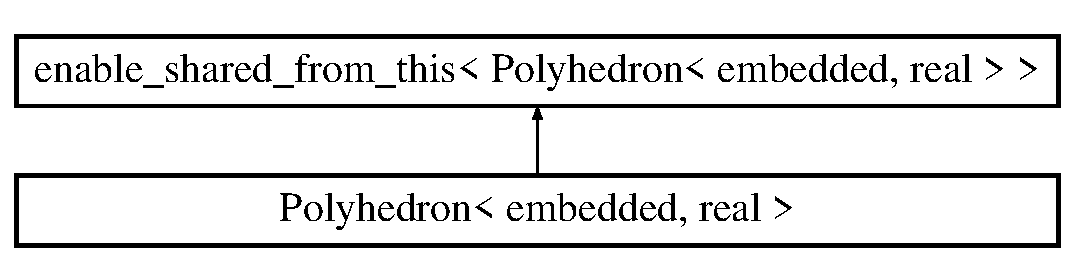
\includegraphics[height=2.000000cm]{class_polyhedron}
\end{center}
\end{figure}
\subsection*{Public Member Functions}
\begin{DoxyCompactItemize}
\item 
\hyperlink{class_polyhedron_ae7091aa1c81e60e701528ed4803f9d20}{Polyhedron} (const private\+Struct \&, const vector$<$ shared\+\_\+ptr$<$ \hyperlink{class_polygon}{Polygon}$<$ embedded, real $>$$>$$>$ \&input\+Polygon\+Vector)
\begin{DoxyCompactList}\small\item\em Constructor from a vector of shared\+\_\+ptr. \end{DoxyCompactList}\item 
\hyperlink{class_polyhedron_a43f9a7fdfcf838c4aa07d95bb3717b51}{Polyhedron} (const private\+Struct \&)
\begin{DoxyCompactList}\small\item\em Empty constructor. \end{DoxyCompactList}\item 
{\footnotesize template$<$typename... Args$>$ }\\\hyperlink{class_polyhedron_a31d0c019cb8aeb7c74d58aa39f91e2f6}{Polyhedron} (const private\+Struct \&, Args...\+arguments)
\begin{DoxyCompactList}\small\item\em Constructor with variadic template. \end{DoxyCompactList}\item 
void \hyperlink{class_polyhedron_a02b8869089bf78342875a197b6995901}{add\+Polygon} (shared\+\_\+ptr$<$ \hyperlink{class_polygon}{Polygon}$<$ embedded, real $>$$>$ \&input\+Polygon)\hypertarget{class_polyhedron_a02b8869089bf78342875a197b6995901}{}\label{class_polyhedron_a02b8869089bf78342875a197b6995901}

\begin{DoxyCompactList}\small\item\em Add a new vertex to the \hyperlink{class_polygon}{Polygon}. \end{DoxyCompactList}\item 
void \hyperlink{class_polyhedron_ad0b79656e93dcd92149f0f3ad53d54e4}{add\+Point} (shared\+\_\+ptr$<$ \hyperlink{class_mesh_point}{Mesh\+Point}$<$ embedded, real $>$$>$ \&input\+Point)\hypertarget{class_polyhedron_ad0b79656e93dcd92149f0f3ad53d54e4}{}\label{class_polyhedron_ad0b79656e93dcd92149f0f3ad53d54e4}

\begin{DoxyCompactList}\small\item\em Add a new \hyperlink{class_polyhedron}{Polyhedron} having this as face. \end{DoxyCompactList}\item 
\hyperlink{class_point}{Point}$<$ embedded, real $>$ \hyperlink{class_polyhedron_a8fa603a39f094cba868b90c5087a9f01}{compute\+Centroid} ()
\item 
real \hyperlink{class_polyhedron_abc5b54102a217358bb0f3af69fdaf6f4}{compute\+Volume} ()
\item 
real \hyperlink{class_polyhedron_acec44568add44445f3d87cc1673083aa}{get\+Diameter} ()
\item 
void \hyperlink{class_polyhedron_ace36af0e1b0638f3a0cb6ac2f828cba9}{fix\+External\+Normal} ()\hypertarget{class_polyhedron_ace36af0e1b0638f3a0cb6ac2f828cba9}{}\label{class_polyhedron_ace36af0e1b0638f3a0cb6ac2f828cba9}

\begin{DoxyCompactList}\small\item\em Makes the normal to each face pointing towards the external of the \hyperlink{class_polyhedron}{Polyhedron}. \end{DoxyCompactList}\item 
void \hyperlink{class_polyhedron_ab5a7edbaf82c77541bb7ed67eef1af78}{fix\+Faces\+Orientation} ()\hypertarget{class_polyhedron_ab5a7edbaf82c77541bb7ed67eef1af78}{}\label{class_polyhedron_ab5a7edbaf82c77541bb7ed67eef1af78}

\begin{DoxyCompactList}\small\item\em Makes the normal of each face pointing in the same direction (or inward or outward) \end{DoxyCompactList}\item 
real \hyperlink{class_polyhedron_ae055b1e499fc2ac20f0db25379c30390}{h\+Triangle} ()
\item 
void {\bfseries initialize} ()\hypertarget{class_polyhedron_a9a64a02c8d5d1afd6c5d0ff4d0b6bcb4}{}\label{class_polyhedron_a9a64a02c8d5d1afd6c5d0ff4d0b6bcb4}

\item 
void {\bfseries link\+Points} ()\hypertarget{class_polyhedron_a2f266d7dac199c4ff5ceb7d06b1c4a3d}{}\label{class_polyhedron_a2f266d7dac199c4ff5ceb7d06b1c4a3d}

\item 
void \hyperlink{class_polyhedron_aafd989af8eb6e5728fd2791049100f41}{link\+Polygons} ()\hypertarget{class_polyhedron_aafd989af8eb6e5728fd2791049100f41}{}\label{class_polyhedron_aafd989af8eb6e5728fd2791049100f41}

\begin{DoxyCompactList}\small\item\em Makes all Polygons pointing to this. \end{DoxyCompactList}\item 
void {\bfseries shrink\+\_\+to\+\_\+fit} ()\hypertarget{class_polyhedron_a4972488920bf2dd7824175435829e475}{}\label{class_polyhedron_a4972488920bf2dd7824175435829e475}

\item 
real {\bfseries space} ()\hypertarget{class_polyhedron_a7b3f6b30e464fd1448d21cb43eb6f80c}{}\label{class_polyhedron_a7b3f6b30e464fd1448d21cb43eb6f80c}

\item 
void \hyperlink{class_polyhedron_a7d8f448cc9f8bbcf4a1e05ee4f8feb2f}{switch\+Faces\+Orientation} ()\hypertarget{class_polyhedron_a7d8f448cc9f8bbcf4a1e05ee4f8feb2f}{}\label{class_polyhedron_a7d8f448cc9f8bbcf4a1e05ee4f8feb2f}

\begin{DoxyCompactList}\small\item\em Invert the orientation of all faces. \end{DoxyCompactList}\item 
void \hyperlink{class_polyhedron_a609105d8805177c2d0e6d7298632a507}{update\+Point\+Vector} ()\hypertarget{class_polyhedron_a609105d8805177c2d0e6d7298632a507}{}\label{class_polyhedron_a609105d8805177c2d0e6d7298632a507}

\begin{DoxyCompactList}\small\item\em If a new face is added, also his vertexes are added to the point\+Vector. \end{DoxyCompactList}\item 
string \hyperlink{class_polyhedron_af611c2257de6a3a6a2f41a0c6c61e118}{write} ()
\begin{DoxyCompactList}\small\item\em Output to string. \end{DoxyCompactList}\item 
bool {\bfseries get\+Is\+Boundary} () const \hypertarget{class_polyhedron_acde3f89641eafdca70566d187f9b5ac7}{}\label{class_polyhedron_acde3f89641eafdca70566d187f9b5ac7}

\item 
void {\bfseries set\+Is\+Boundary} (bool input\+Is\+Boundary)\hypertarget{class_polyhedron_a71d09b5b7f19ef47e9518aa974e9c10c}{}\label{class_polyhedron_a71d09b5b7f19ef47e9518aa974e9c10c}

\item 
real {\bfseries get\+Volume} () const \hypertarget{class_polyhedron_a5fb0dbbf7e0ff2673719623326fb15de}{}\label{class_polyhedron_a5fb0dbbf7e0ff2673719623326fb15de}

\item 
const \hyperlink{class_point}{Point}$<$ embedded, real $>$ \& {\bfseries get\+Centroid} () const \hypertarget{class_polyhedron_a216ab5fbf3fd23a9112a3e1d16ec899d}{}\label{class_polyhedron_a216ab5fbf3fd23a9112a3e1d16ec899d}

\item 
const shared\+\_\+ptr$<$ \hyperlink{class_mesh_point}{Mesh\+Point}$<$ embedded, real $>$ $>$ \& \hyperlink{class_polyhedron_a85926d30dec42f3d8d1c6b5af8a282d3}{point} (long index) const \hypertarget{class_polyhedron_a85926d30dec42f3d8d1c6b5af8a282d3}{}\label{class_polyhedron_a85926d30dec42f3d8d1c6b5af8a282d3}

\begin{DoxyCompactList}\small\item\em Get a shared pointer to a \hyperlink{class_point}{Point} in point\+Vector. \end{DoxyCompactList}\item 
const shared\+\_\+ptr$<$ \hyperlink{class_polygon}{Polygon}$<$ embedded, real $>$ $>$ \& \hyperlink{class_polyhedron_a8aaba4f1c62f24691648ca66419c83fb}{polygon} (long index) const \hypertarget{class_polyhedron_a8aaba4f1c62f24691648ca66419c83fb}{}\label{class_polyhedron_a8aaba4f1c62f24691648ca66419c83fb}

\begin{DoxyCompactList}\small\item\em Get a shared pointer to a \hyperlink{class_polygon}{Polygon} in polygon\+Vector. \end{DoxyCompactList}\item 
shared\+\_\+ptr$<$ \hyperlink{class_polygon}{Polygon}$<$ embedded, real $>$ $>$ \hyperlink{class_polyhedron_a315560a1e132c15d06692a91a6ed69b5}{operator\mbox{[}$\,$\mbox{]}} (long index)\hypertarget{class_polyhedron_a315560a1e132c15d06692a91a6ed69b5}{}\label{class_polyhedron_a315560a1e132c15d06692a91a6ed69b5}

\begin{DoxyCompactList}\small\item\em Get the \hyperlink{class_mesh_point}{Mesh\+Point} with a particular index. \end{DoxyCompactList}\end{DoxyCompactItemize}
\subsection*{Static Public Member Functions}
\begin{DoxyCompactItemize}
\item 
{\footnotesize template$<$typename... Args$>$ }\\static shared\+\_\+ptr$<$ \hyperlink{class_polyhedron}{Polyhedron}$<$ embedded, real $>$ $>$ \hyperlink{class_polyhedron_afa6a4455081915cae5bf082f9f0a8cdf}{make\+\_\+shared\+\_\+\+Polyhedron} (Args...\+arguments)
\begin{DoxyCompactList}\small\item\em The {\bfseries only} constructor for \hyperlink{class_polyhedron}{Polyhedron}. \end{DoxyCompactList}\end{DoxyCompactItemize}
\subsection*{Public Attributes}
\begin{DoxyCompactItemize}
\item 
long \hyperlink{class_polyhedron_ac6c8ccc4248cc0bbf64ef77cc412b844}{number\+Of\+Points}\hypertarget{class_polyhedron_ac6c8ccc4248cc0bbf64ef77cc412b844}{}\label{class_polyhedron_ac6c8ccc4248cc0bbf64ef77cc412b844}

\begin{DoxyCompactList}\small\item\em Number of vertexes. \end{DoxyCompactList}\item 
long \hyperlink{class_polyhedron_a6729506f577ffd64dce9cff14738a26d}{number\+Of\+Polygons}\hypertarget{class_polyhedron_a6729506f577ffd64dce9cff14738a26d}{}\label{class_polyhedron_a6729506f577ffd64dce9cff14738a26d}

\begin{DoxyCompactList}\small\item\em Number of faces. \end{DoxyCompactList}\end{DoxyCompactItemize}
\subsection*{Protected Attributes}
\begin{DoxyCompactItemize}
\item 
vector$<$ shared\+\_\+ptr$<$ \hyperlink{class_polygon}{Polygon}$<$ embedded, real $>$ $>$ $>$ \hyperlink{class_polyhedron_a5079e0df2333cd47e4aa81be382dde10}{polygon\+Vector}\hypertarget{class_polyhedron_a5079e0df2333cd47e4aa81be382dde10}{}\label{class_polyhedron_a5079e0df2333cd47e4aa81be382dde10}

\begin{DoxyCompactList}\small\item\em Stores the faces of the \hyperlink{class_polyhedron}{Polyhedron}. \end{DoxyCompactList}\item 
bool \hyperlink{class_polyhedron_a6ecb308fce1a68cb3cec39c71fe98ddd}{is\+Boundary}\hypertarget{class_polyhedron_a6ecb308fce1a68cb3cec39c71fe98ddd}{}\label{class_polyhedron_a6ecb308fce1a68cb3cec39c71fe98ddd}

\begin{DoxyCompactList}\small\item\em Tells if the \hyperlink{class_polygon}{Polygon} is on the boundary. \end{DoxyCompactList}\item 
real \hyperlink{class_polyhedron_a0f4ab3ccfdc65071201bdb0b55c2b683}{volume}
\item 
\hyperlink{class_point}{Point}$<$ embedded, real $>$ \hyperlink{class_polyhedron_ab7839d59898be24bb956fc41d1c66096}{centroid}
\begin{DoxyCompactList}\small\item\em Not the real centroid, only the mean of the vertexes. \end{DoxyCompactList}\item 
vector$<$ shared\+\_\+ptr$<$ \hyperlink{class_mesh_point}{Mesh\+Point}$<$ embedded, real $>$ $>$ $>$ \hyperlink{class_polyhedron_afda67d1ac832dd4a04539b26aa1ca3f6}{point\+Vector}\hypertarget{class_polyhedron_afda67d1ac832dd4a04539b26aa1ca3f6}{}\label{class_polyhedron_afda67d1ac832dd4a04539b26aa1ca3f6}

\begin{DoxyCompactList}\small\item\em Stores the vertexes of the \hyperlink{class_polyhedron}{Polyhedron}. \end{DoxyCompactList}\end{DoxyCompactItemize}
\subsection*{Friends}
\begin{DoxyCompactItemize}
\item 
{\footnotesize template$<$long embedded2, typename real2 $>$ }\\ostream \& \hyperlink{class_polyhedron_a7aff04af00c6a08042a83db43caa4999}{operator$<$$<$} (ostream \&os, const \hyperlink{class_polyhedron}{Polyhedron}$<$ embedded2, real2 $>$ \&polyhedron)\hypertarget{class_polyhedron_a7aff04af00c6a08042a83db43caa4999}{}\label{class_polyhedron_a7aff04af00c6a08042a83db43caa4999}

\begin{DoxyCompactList}\small\item\em Output operator. \end{DoxyCompactList}\end{DoxyCompactItemize}


\subsection{Detailed Description}
\subsubsection*{template$<$long embedded, typename real = double$>$\\*
class Polyhedron$<$ embedded, real $>$}

Class to represent a \hyperlink{class_polyhedron}{Polyhedron} in 3D. 

The only way to initialize it is to call make\+\_\+shared\+\_\+\+Polygon Volume, faces orientation, normal orientation and centroid are computed during initialization and saved. Inheritance from enable\+\_\+shared\+\_\+from\+\_\+this to obtain a shared\+\_\+ptr from this. 

\subsection{Constructor \& Destructor Documentation}
\index{Polyhedron@{Polyhedron}!Polyhedron@{Polyhedron}}
\index{Polyhedron@{Polyhedron}!Polyhedron@{Polyhedron}}
\subsubsection[{\texorpdfstring{Polyhedron(const private\+Struct \&, const vector$<$ shared\+\_\+ptr$<$ Polygon$<$ embedded, real $>$$>$$>$ \&input\+Polygon\+Vector)}{Polyhedron(const privateStruct &, const vector< shared_ptr< Polygon< embedded, real >>> &inputPolygonVector)}}]{\setlength{\rightskip}{0pt plus 5cm}template$<$long embedded, typename real  = double$>$ {\bf Polyhedron}$<$ embedded, real $>$\+::{\bf Polyhedron} (
\begin{DoxyParamCaption}
\item[{const private\+Struct \&}]{, }
\item[{const vector$<$ shared\+\_\+ptr$<$ {\bf Polygon}$<$ embedded, real $>$$>$$>$ \&}]{input\+Polygon\+Vector}
\end{DoxyParamCaption}
)\hspace{0.3cm}{\ttfamily [inline]}}\hypertarget{class_polyhedron_ae7091aa1c81e60e701528ed4803f9d20}{}\label{class_polyhedron_ae7091aa1c81e60e701528ed4803f9d20}


Constructor from a vector of shared\+\_\+ptr. 

DO N\+OT U\+SE.

Called by make\+\_\+shared\+\_\+\+Polyhedron \index{Polyhedron@{Polyhedron}!Polyhedron@{Polyhedron}}
\index{Polyhedron@{Polyhedron}!Polyhedron@{Polyhedron}}
\subsubsection[{\texorpdfstring{Polyhedron(const private\+Struct \&)}{Polyhedron(const privateStruct &)}}]{\setlength{\rightskip}{0pt plus 5cm}template$<$long embedded, typename real  = double$>$ {\bf Polyhedron}$<$ embedded, real $>$\+::{\bf Polyhedron} (
\begin{DoxyParamCaption}
\item[{const private\+Struct \&}]{}
\end{DoxyParamCaption}
)\hspace{0.3cm}{\ttfamily [inline]}}\hypertarget{class_polyhedron_a43f9a7fdfcf838c4aa07d95bb3717b51}{}\label{class_polyhedron_a43f9a7fdfcf838c4aa07d95bb3717b51}


Empty constructor. 

DO N\+OT U\+SE.

Called by make\+\_\+shared\+\_\+\+Polyhedron \index{Polyhedron@{Polyhedron}!Polyhedron@{Polyhedron}}
\index{Polyhedron@{Polyhedron}!Polyhedron@{Polyhedron}}
\subsubsection[{\texorpdfstring{Polyhedron(const private\+Struct \&, Args...\+arguments)}{Polyhedron(const privateStruct &, Args...arguments)}}]{\setlength{\rightskip}{0pt plus 5cm}template$<$long embedded, typename real  = double$>$ template$<$typename... Args$>$ {\bf Polyhedron}$<$ embedded, real $>$\+::{\bf Polyhedron} (
\begin{DoxyParamCaption}
\item[{const private\+Struct \&}]{, }
\item[{Args...}]{arguments}
\end{DoxyParamCaption}
)\hspace{0.3cm}{\ttfamily [inline]}}\hypertarget{class_polyhedron_a31d0c019cb8aeb7c74d58aa39f91e2f6}{}\label{class_polyhedron_a31d0c019cb8aeb7c74d58aa39f91e2f6}


Constructor with variadic template. 

DO N\+OT U\+SE.

Source\+: \href{http://stackoverflow.com/questions/8158261/templates-how-to-control-number-of-constructor-args-using-template-variable}{\tt http\+://stackoverflow.\+com/questions/8158261/templates-\/how-\/to-\/control-\/number-\/of-\/constructor-\/args-\/using-\/template-\/variable} Called by make\+\_\+shared\+\_\+\+Polyhedron 

\subsection{Member Function Documentation}
\index{Polyhedron@{Polyhedron}!compute\+Centroid@{compute\+Centroid}}
\index{compute\+Centroid@{compute\+Centroid}!Polyhedron@{Polyhedron}}
\subsubsection[{\texorpdfstring{compute\+Centroid()}{computeCentroid()}}]{\setlength{\rightskip}{0pt plus 5cm}template$<$long embedded, typename real $>$ {\bf Point}$<$ embedded, real $>$ {\bf Polyhedron}$<$ embedded, real $>$\+::compute\+Centroid (
\begin{DoxyParamCaption}
{}
\end{DoxyParamCaption}
)}\hypertarget{class_polyhedron_a8fa603a39f094cba868b90c5087a9f01}{}\label{class_polyhedron_a8fa603a39f094cba868b90c5087a9f01}
\begin{DoxyReturn}{Returns}
the centroid 
\end{DoxyReturn}
\index{Polyhedron@{Polyhedron}!compute\+Volume@{compute\+Volume}}
\index{compute\+Volume@{compute\+Volume}!Polyhedron@{Polyhedron}}
\subsubsection[{\texorpdfstring{compute\+Volume()}{computeVolume()}}]{\setlength{\rightskip}{0pt plus 5cm}template$<$long embedded, typename real $>$ real {\bf Polyhedron}$<$ embedded, real $>$\+::compute\+Volume (
\begin{DoxyParamCaption}
{}
\end{DoxyParamCaption}
)}\hypertarget{class_polyhedron_abc5b54102a217358bb0f3af69fdaf6f4}{}\label{class_polyhedron_abc5b54102a217358bb0f3af69fdaf6f4}
\begin{DoxyReturn}{Returns}
the volume of the \hyperlink{class_polyhedron}{Polyhedron} 
\end{DoxyReturn}
\index{Polyhedron@{Polyhedron}!get\+Diameter@{get\+Diameter}}
\index{get\+Diameter@{get\+Diameter}!Polyhedron@{Polyhedron}}
\subsubsection[{\texorpdfstring{get\+Diameter()}{getDiameter()}}]{\setlength{\rightskip}{0pt plus 5cm}template$<$long embedded, typename real $>$ real {\bf Polyhedron}$<$ embedded, real $>$\+::get\+Diameter (
\begin{DoxyParamCaption}
{}
\end{DoxyParamCaption}
)}\hypertarget{class_polyhedron_acec44568add44445f3d87cc1673083aa}{}\label{class_polyhedron_acec44568add44445f3d87cc1673083aa}
\begin{DoxyReturn}{Returns}
the maximum distance between 2 Points 
\end{DoxyReturn}
\index{Polyhedron@{Polyhedron}!h\+Triangle@{h\+Triangle}}
\index{h\+Triangle@{h\+Triangle}!Polyhedron@{Polyhedron}}
\subsubsection[{\texorpdfstring{h\+Triangle()}{hTriangle()}}]{\setlength{\rightskip}{0pt plus 5cm}template$<$long embedded, typename real $>$ real {\bf Polyhedron}$<$ embedded, real $>$\+::h\+Triangle (
\begin{DoxyParamCaption}
{}
\end{DoxyParamCaption}
)}\hypertarget{class_polyhedron_ae055b1e499fc2ac20f0db25379c30390}{}\label{class_polyhedron_ae055b1e499fc2ac20f0db25379c30390}
\begin{DoxyReturn}{Returns}
The maximum distance between vertexes. Necessary for the mesh. 
\end{DoxyReturn}
\index{Polyhedron@{Polyhedron}!make\+\_\+shared\+\_\+\+Polyhedron@{make\+\_\+shared\+\_\+\+Polyhedron}}
\index{make\+\_\+shared\+\_\+\+Polyhedron@{make\+\_\+shared\+\_\+\+Polyhedron}!Polyhedron@{Polyhedron}}
\subsubsection[{\texorpdfstring{make\+\_\+shared\+\_\+\+Polyhedron(\+Args...\+arguments)}{make_shared_Polyhedron(Args...arguments)}}]{\setlength{\rightskip}{0pt plus 5cm}template$<$long embedded, typename real  = double$>$ template$<$typename... Args$>$ static shared\+\_\+ptr$<${\bf Polyhedron}$<$embedded, real$>$ $>$ {\bf Polyhedron}$<$ embedded, real $>$\+::make\+\_\+shared\+\_\+\+Polyhedron (
\begin{DoxyParamCaption}
\item[{Args...}]{arguments}
\end{DoxyParamCaption}
)\hspace{0.3cm}{\ttfamily [inline]}, {\ttfamily [static]}}\hypertarget{class_polyhedron_afa6a4455081915cae5bf082f9f0a8cdf}{}\label{class_polyhedron_afa6a4455081915cae5bf082f9f0a8cdf}


The {\bfseries only} constructor for \hyperlink{class_polyhedron}{Polyhedron}. 

Using the variadic template it accepts as input a vector of shared\+\_\+ptr to Mesh\+Points or a sequence of Mesh\+Points. Then it calls the right constructor. It initialize the \hyperlink{class_polyhedron}{Polyhedron} calling the method initialize

\begin{DoxyReturn}{Returns}
A shared pointer to the \hyperlink{class_polyhedron}{Polyhedron} 
\end{DoxyReturn}
\index{Polyhedron@{Polyhedron}!write@{write}}
\index{write@{write}!Polyhedron@{Polyhedron}}
\subsubsection[{\texorpdfstring{write()}{write()}}]{\setlength{\rightskip}{0pt plus 5cm}template$<$long embedded, typename real $>$ string {\bf Polyhedron}$<$ embedded, real $>$\+::write (
\begin{DoxyParamCaption}
{}
\end{DoxyParamCaption}
)}\hypertarget{class_polyhedron_af611c2257de6a3a6a2f41a0c6c61e118}{}\label{class_polyhedron_af611c2257de6a3a6a2f41a0c6c61e118}


Output to string. 

\begin{DoxyReturn}{Returns}
std\+::string representing the \hyperlink{class_point}{Point} 
\end{DoxyReturn}


\subsection{Member Data Documentation}
\index{Polyhedron@{Polyhedron}!centroid@{centroid}}
\index{centroid@{centroid}!Polyhedron@{Polyhedron}}
\subsubsection[{\texorpdfstring{centroid}{centroid}}]{\setlength{\rightskip}{0pt plus 5cm}template$<$long embedded, typename real  = double$>$ {\bf Point}$<$embedded,real$>$ {\bf Polyhedron}$<$ embedded, real $>$\+::centroid\hspace{0.3cm}{\ttfamily [protected]}}\hypertarget{class_polyhedron_ab7839d59898be24bb956fc41d1c66096}{}\label{class_polyhedron_ab7839d59898be24bb956fc41d1c66096}


Not the real centroid, only the mean of the vertexes. 

\begin{DoxyReturn}{Returns}
the centroid of the \hyperlink{class_polyhedron}{Polyhedron} 
\end{DoxyReturn}
\index{Polyhedron@{Polyhedron}!volume@{volume}}
\index{volume@{volume}!Polyhedron@{Polyhedron}}
\subsubsection[{\texorpdfstring{volume}{volume}}]{\setlength{\rightskip}{0pt plus 5cm}template$<$long embedded, typename real  = double$>$ real {\bf Polyhedron}$<$ embedded, real $>$\+::volume\hspace{0.3cm}{\ttfamily [protected]}}\hypertarget{class_polyhedron_a0f4ab3ccfdc65071201bdb0b55c2b683}{}\label{class_polyhedron_a0f4ab3ccfdc65071201bdb0b55c2b683}
\begin{DoxyReturn}{Returns}
the volume of the \hyperlink{class_polyhedron}{Polyhedron} 
\end{DoxyReturn}


The documentation for this class was generated from the following files\+:\begin{DoxyCompactItemize}
\item 
Mesh\+Point.\+h\item 
Polyhedron.\+h\end{DoxyCompactItemize}

\hypertarget{class_problem}{}\section{Problem$<$ embedded, Mesh\+Type, real $>$ Class Template Reference}
\label{class_problem}\index{Problem$<$ embedded, Mesh\+Type, real $>$@{Problem$<$ embedded, Mesh\+Type, real $>$}}


Virtual class to represent a very generic laplacian problem.  




{\ttfamily \#include $<$Problem.\+h$>$}

Inheritance diagram for Problem$<$ embedded, Mesh\+Type, real $>$\+:\begin{figure}[H]
\begin{center}
\leavevmode
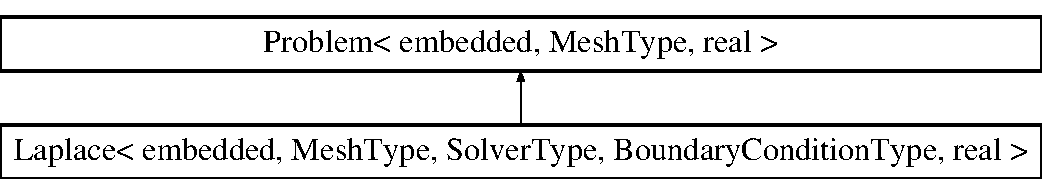
\includegraphics[height=2.000000cm]{class_problem}
\end{center}
\end{figure}
\subsection*{Public Member Functions}
\begin{DoxyCompactItemize}
\item 
\hyperlink{class_problem_a0f93be343a3bc42c319a3f6e43eb86c4}{Problem} (const Mesh\+Type \&input\+Mesh, real input\+Diffusion\+Coeff=1)
\begin{DoxyCompactList}\small\item\em General constructor for the \hyperlink{class_problem}{Problem}. \end{DoxyCompactList}\item 
virtual void \hyperlink{class_problem_a20ac3262ba227f49ff1e1b9765079d59}{compute\+Stiffness\+Matrix} ()=0\hypertarget{class_problem_a20ac3262ba227f49ff1e1b9765079d59}{}\label{class_problem_a20ac3262ba227f49ff1e1b9765079d59}

\begin{DoxyCompactList}\small\item\em Virtual method to compute the stiffness matrix. \end{DoxyCompactList}\item 
virtual void \hyperlink{class_problem_abb49b032c2cd29ed90a1966e3a7a8765}{compute\+Known\+Term} ()=0\hypertarget{class_problem_abb49b032c2cd29ed90a1966e3a7a8765}{}\label{class_problem_abb49b032c2cd29ed90a1966e3a7a8765}

\begin{DoxyCompactList}\small\item\em Virtual method to compute the known term. \end{DoxyCompactList}\item 
virtual void \hyperlink{class_problem_a0eabd7cfaf0b183da21f7246e50abbea}{compute\+Solution} ()\hypertarget{class_problem_a0eabd7cfaf0b183da21f7246e50abbea}{}\label{class_problem_a0eabd7cfaf0b183da21f7246e50abbea}

\begin{DoxyCompactList}\small\item\em Method to compute solution. \end{DoxyCompactList}\item 
virtual void \hyperlink{class_problem_a9fd9a722387afd56922d0327ead502bf}{operator()} ()\hypertarget{class_problem_a9fd9a722387afd56922d0327ead502bf}{}\label{class_problem_a9fd9a722387afd56922d0327ead502bf}

\begin{DoxyCompactList}\small\item\em Method to execute the method. \end{DoxyCompactList}\item 
virtual void \hyperlink{class_problem_a26a9288abd12658a65b26f0a0e42fca5}{display\+Error} (std\+::function$<$ real(\hyperlink{class_point}{Point}$<$ embedded, real $>$ \&)$>$ real\+Solution\+Function)\hypertarget{class_problem_a26a9288abd12658a65b26f0a0e42fca5}{}\label{class_problem_a26a9288abd12658a65b26f0a0e42fca5}

\begin{DoxyCompactList}\small\item\em It displays the error after the computation. \end{DoxyCompactList}\item 
virtual void \hyperlink{class_problem_ad64a7baa630e90b51006b94d76c6943b}{write} (string output\+Points=\char`\"{}points.\+point\char`\"{}, string output\+Connections=\char`\"{}connections.\+conn\char`\"{}, string output\+Solution=\char`\"{}solution.\+sol\char`\"{})\hypertarget{class_problem_ad64a7baa630e90b51006b94d76c6943b}{}\label{class_problem_ad64a7baa630e90b51006b94d76c6943b}

\begin{DoxyCompactList}\small\item\em full Output to file \end{DoxyCompactList}\item 
virtual void \hyperlink{class_problem_a15f66edfd2d8672ed4941b65b03b9750}{write\+Solution} (string output\+Solution=\char`\"{}solution.\+sol\char`\"{})\hypertarget{class_problem_a15f66edfd2d8672ed4941b65b03b9750}{}\label{class_problem_a15f66edfd2d8672ed4941b65b03b9750}

\begin{DoxyCompactList}\small\item\em Output to file of the solution. \end{DoxyCompactList}\end{DoxyCompactItemize}
\subsection*{Public Attributes}
\begin{DoxyCompactItemize}
\item 
Sparse\+Matrix$<$ real $>$ {\bfseries stiffness\+Matrix}\hypertarget{class_problem_ace94c8d8501fde93725f41b0ebd34564}{}\label{class_problem_ace94c8d8501fde93725f41b0ebd34564}

\item 
VectorX$<$ real $>$ {\bfseries known\+Term}\hypertarget{class_problem_a5200b5adea61fcdfc73a1eec0d7074e3}{}\label{class_problem_a5200b5adea61fcdfc73a1eec0d7074e3}

\item 
VectorX$<$ real $>$ {\bfseries solution}\hypertarget{class_problem_a7ac15171e17c2468d35ff477d61b0a57}{}\label{class_problem_a7ac15171e17c2468d35ff477d61b0a57}

\item 
real {\bfseries diffusion\+Coeff}\hypertarget{class_problem_a54bfa04a25f5de579a6128ff871e0b01}{}\label{class_problem_a54bfa04a25f5de579a6128ff871e0b01}

\end{DoxyCompactItemize}
\subsection*{Protected Attributes}
\begin{DoxyCompactItemize}
\item 
const Mesh\+Type \& \hyperlink{class_problem_aee574c7889ffaf5af64338379063dd10}{mesh}\hypertarget{class_problem_aee574c7889ffaf5af64338379063dd10}{}\label{class_problem_aee574c7889ffaf5af64338379063dd10}

\begin{DoxyCompactList}\small\item\em \hyperlink{class_mesh}{Mesh} on which the problem is based. \end{DoxyCompactList}\end{DoxyCompactItemize}


\subsection{Detailed Description}
\subsubsection*{template$<$long embedded, typename Mesh\+Type, typename real = double$>$\\*
class Problem$<$ embedded, Mesh\+Type, real $>$}

Virtual class to represent a very generic laplacian problem. 


\begin{DoxyParams}{Parameters}
{\em embedded} & Dimension of the space \\
\hline
{\em Mesh\+Type} & Type of the file to read \\
\hline
{\em real} & double or long double \\
\hline
\end{DoxyParams}


\subsection{Constructor \& Destructor Documentation}
\index{Problem@{Problem}!Problem@{Problem}}
\index{Problem@{Problem}!Problem@{Problem}}
\subsubsection[{\texorpdfstring{Problem(const Mesh\+Type \&input\+Mesh, real input\+Diffusion\+Coeff=1)}{Problem(const MeshType &inputMesh, real inputDiffusionCoeff=1)}}]{\setlength{\rightskip}{0pt plus 5cm}template$<$long embedded, typename Mesh\+Type , typename real  = double$>$ {\bf Problem}$<$ embedded, Mesh\+Type, real $>$\+::{\bf Problem} (
\begin{DoxyParamCaption}
\item[{const Mesh\+Type \&}]{input\+Mesh, }
\item[{real}]{input\+Diffusion\+Coeff = {\ttfamily 1}}
\end{DoxyParamCaption}
)\hspace{0.3cm}{\ttfamily [inline]}}\hypertarget{class_problem_a0f93be343a3bc42c319a3f6e43eb86c4}{}\label{class_problem_a0f93be343a3bc42c319a3f6e43eb86c4}


General constructor for the \hyperlink{class_problem}{Problem}. 

It allocates the space for all the matrixes 

The documentation for this class was generated from the following files\+:\begin{DoxyCompactItemize}
\item 
Laplace.\+h\item 
Problem.\+h\end{DoxyCompactItemize}

\hypertarget{class_solver}{}\section{Solver$<$ embedded, base\+Element, Matrix\+Type, real $>$ Class Template Reference}
\label{class_solver}\index{Solver$<$ embedded, base\+Element, Matrix\+Type, real $>$@{Solver$<$ embedded, base\+Element, Matrix\+Type, real $>$}}


Generic \hyperlink{class_solver}{Solver} to use in \hyperlink{class_laplace}{Laplace}.  




{\ttfamily \#include $<$Solver.\+h$>$}

\subsection*{Public Member Functions}
\begin{DoxyCompactItemize}
\item 
\hyperlink{class_solver_a0f04e08f93310bc82f9a2efeaffe6db3}{Solver} (std\+::function$<$ real(const \hyperlink{class_point}{Point}$<$ embedded, real $>$ \&)$>$ input\+Force\+Term)\hypertarget{class_solver_a0f04e08f93310bc82f9a2efeaffe6db3}{}\label{class_solver_a0f04e08f93310bc82f9a2efeaffe6db3}

\begin{DoxyCompactList}\small\item\em Very generic constructor. \end{DoxyCompactList}\item 
virtual Matrix\+Type \hyperlink{class_solver_a0049c7be12e2124c717d4db0128ad4b0}{compute\+LocalK} (const shared\+\_\+ptr$<$ base\+Element $>$ \&element)=0
\begin{DoxyCompactList}\small\item\em Main virtual method. \end{DoxyCompactList}\end{DoxyCompactItemize}
\subsection*{Protected Attributes}
\begin{DoxyCompactItemize}
\item 
std\+::function$<$ real(const \hyperlink{class_point}{Point}$<$ embedded, real $>$ \&)$>$ \hyperlink{class_solver_a47ab975c6f2e6312ee5d865d6aec02cd}{force\+Term}\hypertarget{class_solver_a47ab975c6f2e6312ee5d865d6aec02cd}{}\label{class_solver_a47ab975c6f2e6312ee5d865d6aec02cd}

\begin{DoxyCompactList}\small\item\em Force\+Term function to use. \end{DoxyCompactList}\end{DoxyCompactItemize}


\subsection{Detailed Description}
\subsubsection*{template$<$long embedded, typename base\+Element, typename Matrix\+Type, typename real$>$\\*
class Solver$<$ embedded, base\+Element, Matrix\+Type, real $>$}

Generic \hyperlink{class_solver}{Solver} to use in \hyperlink{class_laplace}{Laplace}. 


\begin{DoxyParams}{Parameters}
{\em embedded} & Dimension of the space \\
\hline
{\em base\+Element} & \hyperlink{class_polygon}{Polygon} or \hyperlink{class_polyhedron}{Polyhedron} \\
\hline
{\em Matrix\+Type} & Kind of Matrix to use. \\
\hline
{\em real} & double or long double \\
\hline
\end{DoxyParams}


\subsection{Member Function Documentation}
\index{Solver@{Solver}!compute\+LocalK@{compute\+LocalK}}
\index{compute\+LocalK@{compute\+LocalK}!Solver@{Solver}}
\subsubsection[{\texorpdfstring{compute\+Local\+K(const shared\+\_\+ptr$<$ base\+Element $>$ \&element)=0}{computeLocalK(const shared_ptr< baseElement > &element)=0}}]{\setlength{\rightskip}{0pt plus 5cm}template$<$long embedded, typename base\+Element, typename Matrix\+Type, typename real$>$ virtual Matrix\+Type {\bf Solver}$<$ embedded, base\+Element, Matrix\+Type, real $>$\+::compute\+LocalK (
\begin{DoxyParamCaption}
\item[{const shared\+\_\+ptr$<$ base\+Element $>$ \&}]{element}
\end{DoxyParamCaption}
)\hspace{0.3cm}{\ttfamily [pure virtual]}}\hypertarget{class_solver_a0049c7be12e2124c717d4db0128ad4b0}{}\label{class_solver_a0049c7be12e2124c717d4db0128ad4b0}


Main virtual method. 

To be implemented in subclasses 

Implemented in \hyperlink{class_solver_v_e_m_acdbd3c97184fbd831b2f21e28148c33e}{Solver\+V\+E\+M$<$ embedded, element\+Dimension, base\+Element, Monomial\+Type, real $>$}, \hyperlink{class_solver_v_e_m_acdbd3c97184fbd831b2f21e28148c33e}{Solver\+V\+E\+M$<$ 3, 3, Polyhedron$<$ 3, real $>$, Monomial3\+D$<$ real $>$, real $>$}, and \hyperlink{class_solver_v_e_m_acdbd3c97184fbd831b2f21e28148c33e}{Solver\+V\+E\+M$<$ 2, 2, Polygon$<$ 2, real $>$, Monomial2\+D$<$ real $>$, real $>$}.



The documentation for this class was generated from the following file\+:\begin{DoxyCompactItemize}
\item 
Solver.\+h\end{DoxyCompactItemize}

\hypertarget{class_solver_v_e_m}{}\section{Solver\+V\+EM$<$ embedded, element\+Dimension, base\+Element, Monomial\+Type, real $>$ Class Template Reference}
\label{class_solver_v_e_m}\index{Solver\+V\+E\+M$<$ embedded, element\+Dimension, base\+Element, Monomial\+Type, real $>$@{Solver\+V\+E\+M$<$ embedded, element\+Dimension, base\+Element, Monomial\+Type, real $>$}}


Virtual basic class to solve\+V\+EM.  




{\ttfamily \#include $<$Solver\+V\+E\+M.\+h$>$}

Inheritance diagram for Solver\+V\+EM$<$ embedded, element\+Dimension, base\+Element, Monomial\+Type, real $>$\+:\begin{figure}[H]
\begin{center}
\leavevmode
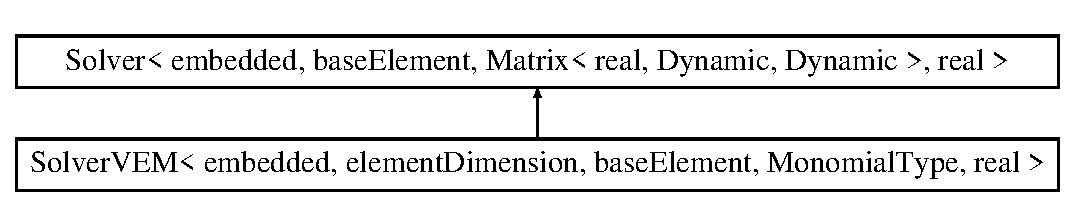
\includegraphics[height=2.000000cm]{class_solver_v_e_m}
\end{center}
\end{figure}
\subsection*{Public Member Functions}
\begin{DoxyCompactItemize}
\item 
\hyperlink{class_solver_v_e_m_ae0eca27b7af4c0877c0abe2cfbcfdcae}{Solver\+V\+EM} (std\+::function$<$ real(const \hyperlink{class_point}{Point}$<$ embedded, real $>$ \&)$>$ input\+Force\+Term)
\begin{DoxyCompactList}\small\item\em Basic constructor. \end{DoxyCompactList}\item 
virtual Matrix$<$ real, Dynamic, Dynamic $>$ \hyperlink{class_solver_v_e_m_acdbd3c97184fbd831b2f21e28148c33e}{compute\+LocalK} (const shared\+\_\+ptr$<$ base\+Element $>$ \&element)\hypertarget{class_solver_v_e_m_acdbd3c97184fbd831b2f21e28148c33e}{}\label{class_solver_v_e_m_acdbd3c97184fbd831b2f21e28148c33e}

\begin{DoxyCompactList}\small\item\em This is to compute the local stiffness matrix. \end{DoxyCompactList}\item 
virtual real \hyperlink{class_solver_v_e_m_af5b39e79f497fb28f63592c44120d5fe}{compute\+Known\+Term} (const shared\+\_\+ptr$<$ base\+Element $>$ \&element, const shared\+\_\+ptr$<$ \hyperlink{class_mesh_point}{Mesh\+Point}$<$ embedded, real $>$$>$ \&point)=0\hypertarget{class_solver_v_e_m_af5b39e79f497fb28f63592c44120d5fe}{}\label{class_solver_v_e_m_af5b39e79f497fb28f63592c44120d5fe}

\begin{DoxyCompactList}\small\item\em Virtual method to compute the known term. \end{DoxyCompactList}\end{DoxyCompactItemize}
\subsection*{Protected Member Functions}
\begin{DoxyCompactItemize}
\item 
virtual Matrix$<$ real, element\+Dimension+1, element\+Dimension+1 $>$ {\bfseries computeG} (Monomial\+Type \&monomial)\hypertarget{class_solver_v_e_m_a65980d6c3c850f5e8d037a9761438e93}{}\label{class_solver_v_e_m_a65980d6c3c850f5e8d037a9761438e93}

\item 
virtual Matrix$<$ real, element\+Dimension+1, Dynamic $>$ {\bfseries computeB} (const shared\+\_\+ptr$<$ base\+Element $>$ \&polyhedron, Monomial\+Type \&monomial)=0\hypertarget{class_solver_v_e_m_a512de296031ac2f954f95c2e78da063d}{}\label{class_solver_v_e_m_a512de296031ac2f954f95c2e78da063d}

\item 
virtual Matrix$<$ real, Dynamic, element\+Dimension+1 $>$ {\bfseries computeD} (Monomial\+Type \&monomial)\hypertarget{class_solver_v_e_m_a73bb74a85b8b436e8e24ed874c8c2ef9}{}\label{class_solver_v_e_m_a73bb74a85b8b436e8e24ed874c8c2ef9}

\item 
virtual Matrix$<$ real, element\+Dimension+1, Dynamic $>$ {\bfseries compute\+P\+I\+Star} (Matrix$<$ real, element\+Dimension+1, element\+Dimension+1 $>$ \&G, Matrix$<$ real, element\+Dimension+1, Dynamic $>$ \&B)\hypertarget{class_solver_v_e_m_a9f092078e8698d00c862e53cae1e20e1}{}\label{class_solver_v_e_m_a9f092078e8698d00c862e53cae1e20e1}

\item 
virtual Matrix$<$ real, Dynamic, Dynamic $>$ {\bfseries compute\+PI} (Matrix$<$ real, element\+Dimension+1, Dynamic $>$ \&P\+I\+Star, Matrix$<$ real, Dynamic, element\+Dimension+1 $>$ \&D)\hypertarget{class_solver_v_e_m_a8d296a88bc9f863fe72688cad49ef2a3}{}\label{class_solver_v_e_m_a8d296a88bc9f863fe72688cad49ef2a3}

\end{DoxyCompactItemize}
\subsection*{Additional Inherited Members}


\subsection{Detailed Description}
\subsubsection*{template$<$long embedded, long element\+Dimension, typename base\+Element, typename Monomial\+Type, typename real = double$>$\\*
class Solver\+V\+E\+M$<$ embedded, element\+Dimension, base\+Element, Monomial\+Type, real $>$}

Virtual basic class to solve\+V\+EM. 

The idea is to implement here all the methods common to 2D and 3D cases and then to specilize the remainings

The methods are mainly methods to compute the characteristics matrixes.


\begin{DoxyParams}{Parameters}
{\em embedded} & Dimension of the space \\
\hline
{\em element\+Dimension} & dimension of each element (2 or 3) \\
\hline
{\em base\+Element} & \hyperlink{class_polygon}{Polygon} or \hyperlink{class_polyhedron}{Polyhedron} \\
\hline
{\em Monomial\+Type} & \hyperlink{class_monomials}{Monomials} or Monomial\+Polygon. The last can be used in case of V\+EM on surfaces \\
\hline
{\em real} & double or long double \\
\hline
\end{DoxyParams}


\subsection{Constructor \& Destructor Documentation}
\index{Solver\+V\+EM@{Solver\+V\+EM}!Solver\+V\+EM@{Solver\+V\+EM}}
\index{Solver\+V\+EM@{Solver\+V\+EM}!Solver\+V\+EM@{Solver\+V\+EM}}
\subsubsection[{\texorpdfstring{Solver\+V\+E\+M(std\+::function$<$ real(const Point$<$ embedded, real $>$ \&)$>$ input\+Force\+Term)}{SolverVEM(std::function< real(const Point< embedded, real > &)> inputForceTerm)}}]{\setlength{\rightskip}{0pt plus 5cm}template$<$long embedded, long element\+Dimension, typename base\+Element, typename Monomial\+Type, typename real = double$>$ {\bf Solver\+V\+EM}$<$ embedded, element\+Dimension, base\+Element, Monomial\+Type, real $>$\+::{\bf Solver\+V\+EM} (
\begin{DoxyParamCaption}
\item[{std\+::function$<$ real(const {\bf Point}$<$ embedded, real $>$ \&)$>$}]{input\+Force\+Term}
\end{DoxyParamCaption}
)\hspace{0.3cm}{\ttfamily [inline]}}\hypertarget{class_solver_v_e_m_ae0eca27b7af4c0877c0abe2cfbcfdcae}{}\label{class_solver_v_e_m_ae0eca27b7af4c0877c0abe2cfbcfdcae}


Basic constructor. 

A lot of paramethers are given as template.


\begin{DoxyParams}{Parameters}
{\em input\+Force\+Term} & std\+::function as force term \\
\hline
\end{DoxyParams}


The documentation for this class was generated from the following file\+:\begin{DoxyCompactItemize}
\item 
Solver\+V\+E\+M.\+h\end{DoxyCompactItemize}

\hypertarget{class_solver_v_e_m2_d}{}\section{Solver\+V\+E\+M2D$<$ real $>$ Class Template Reference}
\label{class_solver_v_e_m2_d}\index{Solver\+V\+E\+M2\+D$<$ real $>$@{Solver\+V\+E\+M2\+D$<$ real $>$}}


Specilized class to solve V\+EM in 2D.  




{\ttfamily \#include $<$Solver\+V\+E\+M2\+D.\+h$>$}

Inheritance diagram for Solver\+V\+E\+M2D$<$ real $>$\+:\begin{figure}[H]
\begin{center}
\leavevmode
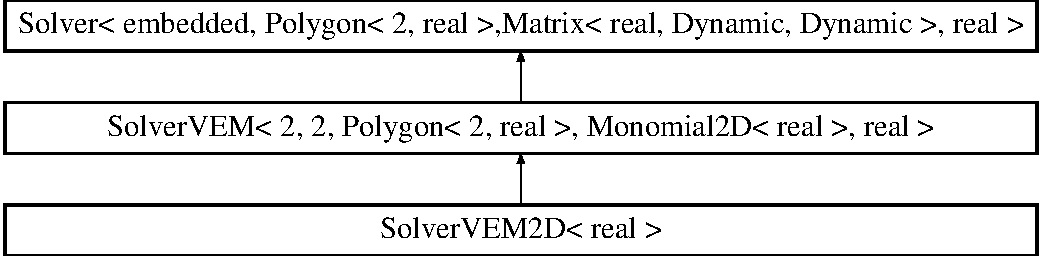
\includegraphics[height=3.000000cm]{class_solver_v_e_m2_d}
\end{center}
\end{figure}
\subsection*{Public Member Functions}
\begin{DoxyCompactItemize}
\item 
virtual Matrix$<$ real, 3, Dynamic $>$ {\bfseries computeB} (const shared\+\_\+ptr$<$ \hyperlink{class_polygon}{Polygon}$<$ 2, real $>$$>$ \&polygon, \hyperlink{class_monomials}{Monomial2D}$<$ real $>$ \&monomial)\hypertarget{class_solver_v_e_m2_d_a047d81b5eda82278be3a2f835dce8845}{}\label{class_solver_v_e_m2_d_a047d81b5eda82278be3a2f835dce8845}

\item 
\hyperlink{class_solver_v_e_m2_d_aaf184f7a8c8d71699aa94cf9f2816e47}{Solver\+V\+E\+M2D} (std\+::function$<$ real(const \hyperlink{class_point}{Point}$<$ 2, real $>$ \&)$>$ input\+Force\+Term)\hypertarget{class_solver_v_e_m2_d_aaf184f7a8c8d71699aa94cf9f2816e47}{}\label{class_solver_v_e_m2_d_aaf184f7a8c8d71699aa94cf9f2816e47}

\begin{DoxyCompactList}\small\item\em Standard constructor. \end{DoxyCompactList}\item 
virtual real \hyperlink{class_solver_v_e_m2_d_a718d3ee9a896d30ee4cbe8a63adf5605}{compute\+Known\+Term} (const shared\+\_\+ptr$<$ \hyperlink{class_polygon}{Polygon}$<$ 2, real $>$$>$ \&element, const shared\+\_\+ptr$<$ \hyperlink{class_mesh_point}{Mesh\+Point}$<$ 2, real $>$$>$ \&point)\hypertarget{class_solver_v_e_m2_d_a718d3ee9a896d30ee4cbe8a63adf5605}{}\label{class_solver_v_e_m2_d_a718d3ee9a896d30ee4cbe8a63adf5605}

\begin{DoxyCompactList}\small\item\em Computes the known term of the element. \end{DoxyCompactList}\end{DoxyCompactItemize}
\subsection*{Additional Inherited Members}


\subsection{Detailed Description}
\subsubsection*{template$<$typename real = double$>$\\*
class Solver\+V\+E\+M2\+D$<$ real $>$}

Specilized class to solve V\+EM in 2D. 

It only implements computeB and compute\+Known\+Term 

The documentation for this class was generated from the following file\+:\begin{DoxyCompactItemize}
\item 
Solver\+V\+E\+M2\+D.\+h\end{DoxyCompactItemize}

\hypertarget{class_solver_v_e_m3_d}{\section{\-Solver\-V\-E\-M3\-D$<$ real $>$ \-Class \-Template \-Reference}
\label{class_solver_v_e_m3_d}\index{\-Solver\-V\-E\-M3\-D$<$ real $>$@{\-Solver\-V\-E\-M3\-D$<$ real $>$}}
}


\-Specilized class to solve \-V\-E\-M in 3\-D.  




{\ttfamily \#include $<$\-Solver\-V\-E\-M3\-D.\-h$>$}

\-Inheritance diagram for \-Solver\-V\-E\-M3\-D$<$ real $>$\-:\begin{figure}[H]
\begin{center}
\leavevmode
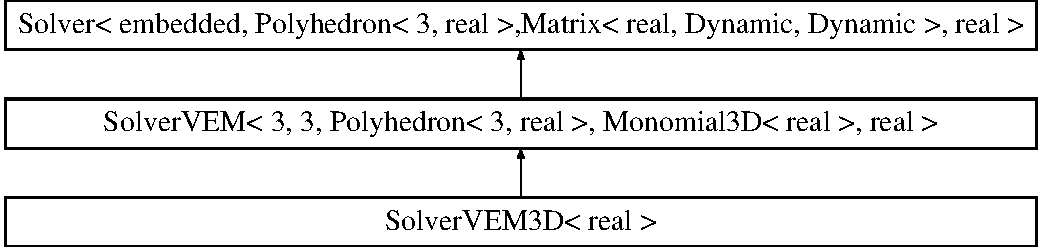
\includegraphics[height=3.000000cm]{class_solver_v_e_m3_d}
\end{center}
\end{figure}
\subsection*{\-Public \-Member \-Functions}
\begin{DoxyCompactItemize}
\item 
virtual \-Matrix$<$ real, 3, 3 $>$ \hyperlink{class_solver_v_e_m3_d_ac318979a89811fbaf443188a13348f8f}{compute\-G\-Polygon} (\hyperlink{class_monomials_polygon}{\-Monomials\-Polygon}$<$ real $>$ \&monomial)
\begin{DoxyCompactList}\small\item\em \-Necessary to use tangential gradient (1-\/\-Nx$\ast$\-Nx) \end{DoxyCompactList}\item 
virtual \-Matrix$<$ real, 4, \-Dynamic $>$ \hyperlink{class_solver_v_e_m3_d_ac87df82bf52bde30ba14e00ca049faf8}{compute\-B} (const shared\-\_\-ptr$<$ \hyperlink{class_polyhedron}{\-Polyhedron}$<$ 3, real $>$$>$ \&polyhedron, \-Monomial3\-D$<$ real $>$ \&monomial)
\begin{DoxyCompactList}\small\item\em \-Complex and computationally expensive function. \end{DoxyCompactList}\item 
\hypertarget{class_solver_v_e_m3_d_afe89753106e3d3be0fdce44620fbbc03}{virtual \-Matrix$<$ real, 3, \-Dynamic $>$ \hyperlink{class_solver_v_e_m3_d_afe89753106e3d3be0fdce44620fbbc03}{compute\-B\-Polygon} (const shared\-\_\-ptr$<$ \hyperlink{class_polygon}{\-Polygon}$<$ 3, real $>$$>$ \&polyhedron, \hyperlink{class_monomials_polygon}{\-Monomials\-Polygon}$<$ real $>$ \&monomial)}\label{class_solver_v_e_m3_d_afe89753106e3d3be0fdce44620fbbc03}

\begin{DoxyCompactList}\small\item\em \-It's an integral on the boundary of a polygon. \-Similar to the compute\-B in the 2\-D case. \end{DoxyCompactList}\item 
\hypertarget{class_solver_v_e_m3_d_a390dd7d1654bee6686b76e6a08579416}{virtual \-Matrix$<$ real, \-Dynamic, 3 $>$ \hyperlink{class_solver_v_e_m3_d_a390dd7d1654bee6686b76e6a08579416}{compute\-D\-Polygon} (\hyperlink{class_monomials_polygon}{\-Monomials\-Polygon}$<$ real $>$ \&monomial)}\label{class_solver_v_e_m3_d_a390dd7d1654bee6686b76e6a08579416}

\begin{DoxyCompactList}\small\item\em \-Similar to compute\-D in the standard case. \end{DoxyCompactList}\item 
\hypertarget{class_solver_v_e_m3_d_ae5ebe2417660a9688446d93e998579cc}{virtual \-Matrix$<$ real, 3, \-Dynamic $>$ {\bfseries compute\-P\-I\-Star\-Polygon} (\-Matrix$<$ real, 3, 3 $>$ \&\-G, \-Matrix$<$ real, 3, \-Dynamic $>$ \&\-B)}\label{class_solver_v_e_m3_d_ae5ebe2417660a9688446d93e998579cc}

\item 
\hypertarget{class_solver_v_e_m3_d_ab47c381f6c5708f5d6874f7b22c8d0d9}{\hyperlink{class_solver_v_e_m3_d_ab47c381f6c5708f5d6874f7b22c8d0d9}{\-Solver\-V\-E\-M3\-D} (std\-::function$<$ real(const \hyperlink{class_point}{\-Point}$<$ 3, real $>$ \&)$>$ input\-Force\-Term)}\label{class_solver_v_e_m3_d_ab47c381f6c5708f5d6874f7b22c8d0d9}

\begin{DoxyCompactList}\small\item\em \-Standard constructor. \end{DoxyCompactList}\item 
virtual real \hyperlink{class_solver_v_e_m3_d_ae11471f960f7c4677778dd52d8ce1bd5}{compute\-Known\-Term} (const shared\-\_\-ptr$<$ \hyperlink{class_polyhedron}{\-Polyhedron}$<$ 3, real $>$$>$ \&element, const shared\-\_\-ptr$<$ \hyperlink{class_mesh_point}{\-Mesh\-Point}$<$ 3, real $>$$>$ \&point)
\begin{DoxyCompactList}\small\item\em 3\-D version of comute\-Known\-Term \end{DoxyCompactList}\end{DoxyCompactItemize}


\subsection{\-Detailed \-Description}
\subsubsection*{template$<$typename real = double$>$class Solver\-V\-E\-M3\-D$<$ real $>$}

\-Specilized class to solve \-V\-E\-M in 3\-D. 

\-Complex way of computing \-B. \-The boundary term requires to compute an interpolating polynomial on the face. \-This requires to solve a \-V\-E\-M-\/like problem on the face to compute the polynomial. \-It's the computational most expensive part. 

\subsection{\-Member \-Function \-Documentation}
\hypertarget{class_solver_v_e_m3_d_ac87df82bf52bde30ba14e00ca049faf8}{\index{\-Solver\-V\-E\-M3\-D@{\-Solver\-V\-E\-M3\-D}!compute\-B@{compute\-B}}
\index{compute\-B@{compute\-B}!SolverVEM3D@{\-Solver\-V\-E\-M3\-D}}
\subsubsection[{compute\-B}]{\setlength{\rightskip}{0pt plus 5cm}template$<$typename real $>$ \-Matrix$<$ real, 4, \-Dynamic $>$ {\bf \-Solver\-V\-E\-M3\-D}$<$ real $>$\-::{\bf compute\-B} (
\begin{DoxyParamCaption}
\item[{const shared\-\_\-ptr$<$ {\bf \-Polyhedron}$<$ 3, real $>$$>$ \&}]{polyhedron, }
\item[{\-Monomial3\-D$<$ real $>$ \&}]{monomial}
\end{DoxyParamCaption}
)\hspace{0.3cm}{\ttfamily  \mbox{[}virtual\mbox{]}}}}\label{class_solver_v_e_m3_d_ac87df82bf52bde30ba14e00ca049faf8}


\-Complex and computationally expensive function. 

2 ways of computing the boundary term
\begin{DoxyItemize}
\item 
\end{DoxyItemize}\hypertarget{class_solver_v_e_m3_d_ac318979a89811fbaf443188a13348f8f}{\index{\-Solver\-V\-E\-M3\-D@{\-Solver\-V\-E\-M3\-D}!compute\-G\-Polygon@{compute\-G\-Polygon}}
\index{compute\-G\-Polygon@{compute\-G\-Polygon}!SolverVEM3D@{\-Solver\-V\-E\-M3\-D}}
\subsubsection[{compute\-G\-Polygon}]{\setlength{\rightskip}{0pt plus 5cm}template$<$typename real $>$ \-Matrix$<$ real, 3, 3 $>$ {\bf \-Solver\-V\-E\-M3\-D}$<$ real $>$\-::{\bf compute\-G\-Polygon} (
\begin{DoxyParamCaption}
\item[{{\bf \-Monomials\-Polygon}$<$ real $>$ \&}]{monomial}
\end{DoxyParamCaption}
)\hspace{0.3cm}{\ttfamily  \mbox{[}virtual\mbox{]}}}}\label{class_solver_v_e_m3_d_ac318979a89811fbaf443188a13348f8f}


\-Necessary to use tangential gradient (1-\/\-Nx$\ast$\-Nx) 

\-The product of the gradient of x with the gradient of y is \-N\-O\-T 0. \-I have to project it on the plane. \hypertarget{class_solver_v_e_m3_d_ae11471f960f7c4677778dd52d8ce1bd5}{\index{\-Solver\-V\-E\-M3\-D@{\-Solver\-V\-E\-M3\-D}!compute\-Known\-Term@{compute\-Known\-Term}}
\index{compute\-Known\-Term@{compute\-Known\-Term}!SolverVEM3D@{\-Solver\-V\-E\-M3\-D}}
\subsubsection[{compute\-Known\-Term}]{\setlength{\rightskip}{0pt plus 5cm}template$<$typename real $>$ real {\bf \-Solver\-V\-E\-M3\-D}$<$ real $>$\-::{\bf compute\-Known\-Term} (
\begin{DoxyParamCaption}
\item[{const shared\-\_\-ptr$<$ {\bf \-Polyhedron}$<$ 3, real $>$$>$ \&}]{element, }
\item[{const shared\-\_\-ptr$<$ {\bf \-Mesh\-Point}$<$ 3, real $>$$>$ \&}]{point}
\end{DoxyParamCaption}
)\hspace{0.3cm}{\ttfamily  \mbox{[}virtual\mbox{]}}}}\label{class_solver_v_e_m3_d_ae11471f960f7c4677778dd52d8ce1bd5}


3\-D version of comute\-Known\-Term 

\-First order formula\-: it computes f in the average of the vertexes. \-In many cases this is the centroid so the formula becomes second order. \-It would be too expensive to compute the real centroid for each polyhedron. \-Moreover we used first order \-V\-E\-M, so there is no reason to increase the order of this formula 

\-The documentation for this class was generated from the following file\-:\begin{DoxyCompactItemize}
\item 
\-Solver\-V\-E\-M3\-D.\-h\end{DoxyCompactItemize}

\printindex
\end{document}
